\documentclass{article}
\usepackage{ifluatex}
\ifluatex 
    \usepackage{fontspec}
    \setsansfont{CMU Sans Serif}%{Arial}
    \setmainfont{CMU Serif}%{Times New Roman}
    \setmonofont{CMU Typewriter Text}%{Consolas}
    \defaultfontfeatures{Ligatures={TeX}}
\else
    \usepackage[T2A]{fontenc}
    \usepackage[utf8]{inputenc}
\fi
\usepackage[english,russian]{babel}
\usepackage{amssymb,latexsym,amsmath,amscd,mathtools,wasysym}
\usepackage[shortlabels]{enumitem}
\usepackage[makeroom]{cancel}
\usepackage{graphicx}
\usepackage{geometry}
\usepackage{verbatim}
\usepackage{fvextra}

\usepackage{longtable}
\usepackage{multirow}
\usepackage{multicol}
\usepackage{tabu}
\usepackage{arydshln} % \hdashline and :

\usepackage{float}
\makeatletter
\g@addto@macro\@floatboxreset\centering
\makeatother
\usepackage{caption}
\usepackage{csquotes}
\usepackage[bb=dsserif]{mathalpha}
\usepackage[normalem]{ulem}

\usepackage[e]{esvect}
\let\vec\vv

\usepackage{xcolor}
\colorlet{darkgreen}{black!25!blue!50!green}


%% Here f*cking with mathabx
\DeclareFontFamily{U}{matha}{\hyphenchar\font45}
\DeclareFontShape{U}{matha}{m}{n}{
    <5> <6> <7> <8> <9> <10> gen * matha
    <10.95> matha10 <12> <14.4> <17.28> <20.74> <24.88> matha12
}{}
\DeclareSymbolFont{matha}{U}{matha}{m}{n}
\DeclareFontFamily{U}{mathb}{\hyphenchar\font45}
\DeclareFontShape{U}{mathb}{m}{n}{
    <5> <6> <7> <8> <9> <10> gen * mathb
    <10.95> matha10 <12> <14.4> <17.28> <20.74> <24.88> mathb12
}{}
\DeclareSymbolFont{mathb}{U}{mathb}{m}{n}

\DeclareMathSymbol{\defeq}{\mathrel}{mathb}{"15}
\DeclareMathSymbol{\eqdef}{\mathrel}{mathb}{"16}


\usepackage{trimclip}
\DeclareMathOperator{\updownarrows}{\clipbox{0pt 0pt 4.175pt 0pt}{$\upuparrows$}\hspace{-.825px}\clipbox{0pt 0pt 4.175pt 0pt}{$\downdownarrows$}}
\DeclareMathOperator{\downuparrows}{\clipbox{0pt 0pt 4.175pt 0pt}{$\downdownarrows$}\hspace{-.825px}\clipbox{0pt 0pt 4.175pt 0pt}{$\upuparrows$}}

\makeatletter
\providecommand*\deletecounter[1]{%
    \expandafter\let\csname c@#1\endcsname\@undefined}
\makeatother


\usepackage{hyperref}
\hypersetup{
    %hidelinks,
    colorlinks=true,
    linkcolor=darkgreen,
    urlcolor=blue,
    breaklinks=true,
}

\usepackage{pgf}
\usepackage{pgfplots}
\pgfplotsset{compat=newest}
\usepackage{tikz,tikz-3dplot}
\usepackage{tkz-euclide}
\usetikzlibrary{calc,automata,patterns,angles,backgrounds,shapes.geometric,trees,positioning,decorations.pathreplacing}
\pgfkeys{/pgf/plot/gnuplot call={T: && cd TeX && gnuplot}}
\usepgfplotslibrary{fillbetween,polar}
\ifluatex
\usetikzlibrary{graphs,graphs.standard,graphdrawing,quotes,babel}
\usegdlibrary{trees,force,circular}
\else

\fi
\makeatletter
\newcommand\currentnode{\the\tikz@lastxsaved,\the\tikz@lastysaved}
\makeatother

%\usepgfplotslibrary{external} 
%\tikzexternalize

\makeatletter
\newcommand*\circled[2][1.0]{\tikz[baseline=(char.base)]{
        \node[shape=circle, draw, inner sep=2pt,
        minimum height={\f@size*#1},] (char) {#2};}}
\makeatother

\newcommand{\existence}{{\circled{$\exists$}}}
\newcommand{\uniqueness}{{\circled{$\hspace{0.5px}!$}}}
\newcommand{\rightimp}{{\circled{$\Rightarrow$}}}
\newcommand{\leftimp}{{\circled{$\Leftarrow$}}}

\DeclareMathOperator{\sign}{sign}
\DeclareMathOperator{\Cl}{Cl}
\DeclareMathOperator{\proj}{pr}
\DeclareMathOperator{\Arg}{Arg}
\DeclareMathOperator{\supp}{supp}
\DeclareMathOperator{\diag}{diag}
\DeclareMathOperator{\tr}{tr}
\DeclareMathOperator{\rank}{rank}
\DeclareMathOperator{\Lat}{Lat}
\DeclareMathOperator{\Lin}{Lin}
\DeclareMathOperator{\Ln}{Ln}
\DeclareMathOperator{\Orbit}{Orbit}
\DeclareMathOperator{\St}{St}
\DeclareMathOperator{\Seq}{Seq}
\DeclareMathOperator{\PSet}{PSet}
\DeclareMathOperator{\MSet}{MSet}
\DeclareMathOperator{\Cyc}{Cyc}
\DeclareMathOperator{\Hom}{Hom}
\DeclareMathOperator{\End}{End}
\DeclareMathOperator{\Aut}{Aut}
\DeclareMathOperator{\Ker}{Ker}
\DeclareMathOperator{\Def}{def}
\DeclareMathOperator{\Alt}{Alt}
\DeclareMathOperator{\Sim}{Sim}
\DeclareMathOperator{\Int}{Int}
\DeclareMathOperator{\grad}{grad}
\DeclareMathOperator{\sech}{sech}
\DeclareMathOperator{\csch}{csch}
\DeclareMathOperator{\asin}{\sin^{-1}}
\DeclareMathOperator{\acos}{\cos^{-1}}
\DeclareMathOperator{\atan}{\tan^{-1}}
\DeclareMathOperator{\acot}{\cot^{-1}}
\DeclareMathOperator{\asec}{\sec^{-1}}
\DeclareMathOperator{\acsc}{\csc^{-1}}
\DeclareMathOperator{\asinh}{\sinh^{-1}}
\DeclareMathOperator{\acosh}{\cosh^{-1}}
\DeclareMathOperator{\atanh}{\tanh^{-1}}
\DeclareMathOperator{\acoth}{\coth^{-1}}
\DeclareMathOperator{\asech}{\sech^{-1}}
\DeclareMathOperator{\acsch}{\csch^{-1}}

\newcommand*{\scriptA}{{\mathcal{A}}}
\newcommand*{\scriptB}{{\mathcal{B}}}
\newcommand*{\scriptC}{{\mathcal{C}}}
\newcommand*{\scriptD}{{\mathcal{D}}}
\newcommand*{\scriptF}{{\mathcal{F}}}
\newcommand*{\scriptH}{{\mathcal{H}}}
\newcommand*{\scriptK}{{\mathcal{K}}}
\newcommand*{\scriptL}{{\mathcal{L}}}
\newcommand*{\scriptM}{{\mathcal{M}}}
\newcommand*{\scriptP}{{\mathcal{P}}}
\newcommand*{\scriptQ}{{\mathcal{Q}}}
\newcommand*{\scriptR}{{\mathcal{R}}}
\newcommand*{\scriptT}{{\mathcal{T}}}
\newcommand*{\scriptU}{{\mathcal{U}}}
\newcommand*{\scriptX}{{\mathcal{X}}}
\newcommand*{\Cnk}[2]{\left(\begin{matrix}#1\\#2\end{matrix}\right)}
\newcommand*{\im}{{\mathbf i}}
\newcommand*{\id}{{\mathrm{id}}}
\newcommand*{\compl}{^\complement}
\newcommand*{\dotprod}[2]{{\left\langle{#1},{#2}\right\rangle}}
\newcommand\matr[1]{\left(\begin{matrix}#1\end{matrix}\right)}
\newcommand\matrd[1]{\left|\begin{matrix}#1\end{matrix}\right|}
\newcommand\arr[2]{\left(\begin{array}{#1}#2\end{array}\right)}

\DeclareMathOperator{\divby}{\scalebox{1}[.65]{\vdots}}
\DeclareMathOperator{\toto}{\rightrightarrows}
\DeclareMathOperator{\ntoto}{\not\rightrightarrows}

\newcommand{\undercolorblack}[2]{{\color{#1}\underline{\color{black}#2}}}
\newcommand{\undercolor}[2]{{\colorlet{tmp}{.}\color{#1}\underline{\color{tmp}#2}}}
\newcommand{\swift}[1]{\mintinline{swift}{#1}}

\usepackage{adjustbox}

\geometry{margin=1in}
\usepackage{fancyhdr}
\pagestyle{fancy}
\fancyfoot[L]{}
\fancyfoot[C]{Корнильев Артемий}
\fancyfoot[R]{\pagename\ \thepage}
\fancyhead[L]{}
\fancyhead[R]{\leftmark}
\renewcommand{\sectionmark}[1]{\markboth{#1}{}}

\setcounter{tocdepth}{5}
\newcommand{\convexpath}[2]{
    [   
    create hullcoords/.code={
        \global\edef\namelist{#1}
        \foreach [count=\counter] \nodename in \namelist {
            \global\edef\numberofnodes{\counter}
            \coordinate (hullcoord\counter) at (\nodename);
        }
        \coordinate (hullcoord0) at (hullcoord\numberofnodes);
        \pgfmathtruncatemacro\lastnumber{\numberofnodes+1}
        \coordinate (hullcoord\lastnumber) at (hullcoord1);
    },
    create hullcoords
    ]
    ($(hullcoord1)!#2!-90:(hullcoord0)$)
    \foreach [
    evaluate=\currentnode as \previousnode using \currentnode-1,
    evaluate=\currentnode as \nextnode using \currentnode+1
    ] \currentnode in {1,...,\numberofnodes} {
        let \p1 = ($(hullcoord\currentnode) - (hullcoord\previousnode)$),
        \n1 = {atan2(\y1,\x1) + 90},
        \p2 = ($(hullcoord\nextnode) - (hullcoord\currentnode)$),
        \n2 = {atan2(\y2,\x2) + 90},
        \n{delta} = {Mod(\n2-\n1,360) - 360}
        in 
        {arc [start angle=\n1, delta angle=\n{delta}, radius=#2]}
        -- ($(hullcoord\nextnode)!#2!-90:(hullcoord\currentnode)$) 
    }
} % Nodes CW. Supposes tikz >= 3.0, else swap atan2 arguments.


\tikzset{treenode/.style={
        inner sep=0pt,
        text width=5mm,
        scale=.8,
        circle,
        outer sep=2mm,
        align=center,
        draw=black,
        fill=white,
        thin
}}
\tikzset{subtree/.style={
        regular polygon,
        regular polygon sides=3,
        inner sep=0pt,
        text width=5mm,
        yscale=1.5,
        xscale=.7,
        draw=black,
        fill=white,
        thin
}}
\tikzset{
    ->-/.style={
        decoration={
            markings,
            mark=at position #1 with {\arrow{>}}
        },
        postaction={decorate}
    },
    ->-/.default=0.5,
    -<-/.style={
        decoration={
            markings,
            mark=at position #1 with {\arrow{<}}
        },
        postaction={decorate}
    },
    -<-/.default=0.5
}

\usepackage{amsthm}
\usepackage{chngcntr}

\theoremstyle{definition}
\newtheorem{definition}{Определение}
\counterwithin*{definition}{section}

\theoremstyle{plain}
\newtheorem{theorem}{Теорема}
\counterwithin*{theorem}{section} % Without changing appearance
\newtheorem{lemma}{Лемма}
\counterwithin*{lemma}{section}
\newtheorem{corollary}{Следствие}[theorem]
\counterwithin{corollary}{theorem} % Changing appearance
\counterwithin{corollary}{lemma}
\newtheorem*{claim}{Утверждение}
\newtheorem{property}{Свойство}[definition]

\theoremstyle{remark}
\newtheorem*{remark}{Замечание}
\newtheorem*{example}{Пример}


%\renewcommand\qedsymbol{$\blacksquare$}

\counterwithin{equation}{section}


\usepackage[cache=true]{minted}
\usemintedstyle{tango}

\fancyhead[L]{iOS, конспект второй,от Яндекса}

\begin{document}
    \tableofcontents\pagebreak
    \section{Лекция первая, введение в систему}
    \subsection{Минутка истории}
    Раньше, во времена, когда вышел первый айфон, на айфон можно было писать только веб приложения. Делать это можно и сегодня, но так перестали делать из-за низкой производительности(браузер съедает ресурсы) + недостаточная функциональность, ограниченная работа в режиме offline так как сайтам нужно постоянное подключение к интернету + невозможность контролировать качество, нет никакого рейтинга. 
    \newline
    Но apple все равно развивает эту индустрию, с iOS15 появились WebExtensions, а с iOS 16.4: WebPushes, сайты могут присылать уведомления. 
    \newline
    Далее с появлением iphoneOS 2, появилась и СДК, называлась библиотека Cocoa touch. С этого момента начинается история iOS разработки. Cocoa touch -- фреймворк, который помогал писать код под айфоны, хорошо продуманных архитектур не было. 
    \newline
    Далее, вместе с iOS3 появлись iPad. 
    \newline
    С iOS 4 появились блоки и arc. В iOS появилась многопоточка и потребовался понятный и удобный способ с ней взаимодействовать. 
    \newline
    С iOS 6 мы имеем все технологии, которые позволяют делать нам приложение. 
    \subsection{Разбираемся с XCode}
    Вообще, первый раз когда мы создаем приложение, перед нами вот такая картина:
    \newline
    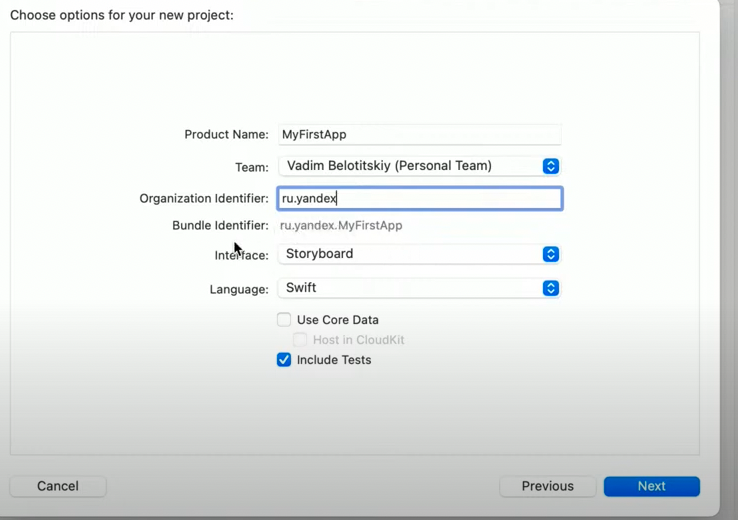
\includegraphics[scale = 0.5]{pic/xcodeOpen.png}
    \newline
    Соответсвенно, разберем каждый из пунктов. 
    \newline
    \textbf{Product name --} просто имя нашего проэкта. \textbf{идентификатор организации} -- можно писать все что угодно. \textbf{Bundle identifier -- } тут интереснее, это полный id-шник пакеты, через который распространяются наши приложения. Он уникален для каждого приложения, если какой-то занят, нам нужно придумать новый, потому что врятли такое приложение мы сможем зарегестрировать в app store.
    \newline
    \textbf{Interface --} выбираем interface, либо UIKit(storyboard), либо SwiftUI.
    \newline
    Точка входа в приложение находится в файле \textbf{App Delegate}, он у нас помечен директивой \swift{@main}, это значит, что будет сгенерирован компилятором код, который будет вызывать \swift{UIApplicationMain}. Можно использовать как директиву, так и функцию, но как правило функция не требуется, она может понадобится, только если мы захотим подменить класс приложения, но обычно этого не требуется. 
    \newline
    \textbf{Bundle Identifier } можно поменять в корневом файле проэкта во вкладке \textbf{Build Settings}.
    \newline
    \textbf{Target --} набор классов, которые устанавливаются на симулятор. 
    \newline
    \textbf{Assets --} сущность, в которую мы складываем картинки, которые попадают в bundle приложения, после чего их можно оттуда вызывать, и использовать на экране. Также создав какую то новую картинку мы можем увидеть 1х, 2х и 3х. Это просто разные масштабы одной картинки. Допустим картинка у нас 300/300 пикселей. Тогда в 2х мы закинем нашу же картинку но 600/600 и тд. Можно еще использовать веткорные изображения, но впоследствии они все равно превращаются в растровые, что только замедляет компиляцию.
    \newline
    \textbf{SceneDelegate --} занимается входами и выходами из бекграунда. Сущность, которая привязывается к экрану, как правило в нее пишется простой код, как правило мы отслеживаем переход из состояния active или уход в него, береход в состояние background. Используется для обработки событий. Если мы хотим все создавать из кода, то SceneDelegate это и будет нашей точкой входа в приложение. 
    \section{Лекция 2, программирование на swift}
    \subsection{Value type и Reference type}
    Все типы в swift делятся на value(значение) и reference(ссылочные). K reference типам относятся классы, замыкания, функции и actorы. К value типам -- все остальные. 
    \newline
    \textbf{Value type} имеет семантику копирования, то есть каждый раз, когда мы передаем экземпляр этой переменной в функцию или в новую переменную, создается ее новый экземпляр. Рассмотрим следующий пример: 
    \begin{minted}{swift}
        struct Cup{
            var isFilled:Bool = false
            mutating func fill(){ //для того, чтобы менять какой-то свойство если мы работаем
            //со структурами или enum, необходимо использовать ключевое слово mutating
                isFilled = true       
            }
        }
        let cup1 = Cup()
        var cup2 = cup1
        cup2.fill() //свойство isFilled поменялось для одной чашки, но для другой осталось прежним
        //так как в данном случае мы работали с копией 
        print(cup1.isFilled)//false
        print(cup2.isFilled)//true
    \end{minted}
    Теперь поймем разницу между reference type написав то же самое, но использовав \swift{class}.
    \begin{minted}{swift}
        class Cup{
            var isFilled:Bool = false
             func fill(){ //для того, чтобы менять какой-то свойство если мы работаем
             //со структурами или enum, необходимо использовать ключевое слово mutating
                isFilled = true       
            }
        }
        let cup1 = Cup()
        var cup2 = cup1
        cup2.fill() 
        print(cup1.isFilled)//true 
        print(cup2.isFilled)//true 
        // в обоих случаях true так как в данном случае мы работали с одной чашкой.
    \end{minted}
    Большинство стандартных типов, которые мы используем каждый день на самом деле являются структурами. 
    \newline
    Чтобы каждый раз не создавать новый объект и не забивать память стандартные структуры в Swift такие как array, set, dictionary, string поддерживают механизм Copy-on-write. Как он работает, разберем на примере: 
    \begin{minted}{swift}
        var array1 = [0, 1, 2, 3]
        var array2 = array1
        array2.append(4)
        //как только мы добавили что-то в array2 создается копия динамического буфера и она меняется. Мы не создаем копию до тех пор, пока не хотим поменять какой-то экземпляр. 
    \end{minted}
    Такой механизм можно реализовать и для своих собственных типов. 
    \subsection{Свойства}
    Классы, структуры, enum могут содержать свойства. Они бывают двух видом: хранимые и вычислимые. Хранимые выступают константами, так же мы можем сделать lazy хранимое свойство, его значение будет установлено при первом обращении к нему. 
    \textbf{Выячислимые свойства --} свойства, которые не хранят что-то, а динамически это вычисляют каждый раз при обращении. Они делают это в блоке get. Пример каждого можно рассмотреть на этой картинке: 
    \newline
    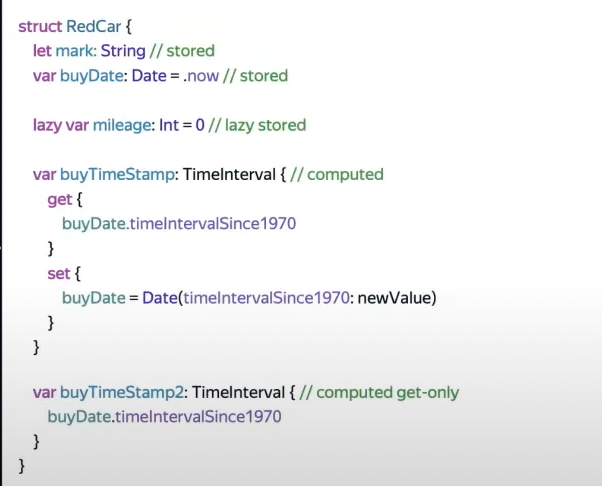
\includegraphics[scale = 0.5]{pic/propsAdvSwift.png}
    \newline
    В swift методы могут генерировать ошибки и возвращать их в область вызова этого метода. Computed property также могут делать это в блоке get, для этого нужно использовать после ключевое слово throws. Есть одно важное ограничение: оно не может содержать блок set.
    \begin{minted}{swift}
        enum ValueError: Error{
            case randomError            
        }
        struct A{
            var randomL:Int{
                get throws{
                    if Bool.random(){
                        throw ValueError.randomError
                    }
                }
                return 10
            }
        }
    \end{minted}
    Помимо свойств и метода экземпляра есть свойства и методы типов. Чтобы их использовать мы обращаемся напрямую к типу и не создаем экземпляр, они отличаются ключевыми словами \swift{class} и \swift{static}.
    \newline
    \swift{static} определяет свойство типа и доступно в классах, структурах и enum-ах. 
    \newline
    \swift{class} доступно только в классах. В swift классы поддерживают наследование, при этом наследоваться можно только от одного класса. Это ключевое слово позволяет переопределить какое либо свойство в классе наследнике. Может применяться только для вычислимых свойств или методах.
    \newline
    Когда мы хотим переопределить метод при наследовании мы пишем ключевое слово override и необходимую сигнатуру, пишем новую реализацию и все. 
    \newline
    Со свойствами немного сложнее, свойства мы можем переопределить двумя способами: 
    \newline 
    1) Переопределить как вычислимое свойство: 
    \begin{minted}{swift}
        class Car{
            var startPrice:Int = 100
            class var productionAmount:Int{
                100000
            }
            var coefficient: Int = 2
            var price: Int{
                get{
                    startPrice * coefficient
                }
                set{
                    coefficient = newValue
                }
            }
            func drive(){
                print("Driving")
            }
        }

        class Tesla: Car{
            override func drive(){
                print("Tesla driving")
            }
            //Tesla -- наследник car, мы хотим переопределить свойство ниже
            //В классе родителя оно было доступно только для чтения, такой свойство мы можем 
            //переопределить как доступное только для чтения, либо только для чтения и для изменения
            //также это было свойство типа, отмеченной ключевым словом class
            //мы можем его переопределить как с использованием ключевого слова static, так и class.
            //В данном случае использовали static, чтобы избежать дальнейшего переопределения. 
            
            override static var productionAmount: Int{
                super.productionAmount + 200
            }
            //Также мы хотим переопределить свойство price.
            //В классе родителя оно было доступно как для чтения так и для определения, поэтому только для чтения переопредлить мы его не можем. 
            override var price: Int{
                super.price + 20
            }
        }
    \end{minted}  
    Второй способ переопределения свойств: добавить к ним наблюдателей свойств. Это позволит получать уведомление об изменении значения наследуемого свойства, независимо от того, как оно было реализовано изначально. 
    \begin{minted}{swift}
        class Car{
            var startPrice: Int = 100
        }
        class Tesla: Car{
            override var startPrice: Int{
                willSet{
                    print("New startPrice \(newValue)")
                }
                didSet{
                    print("Old startPrice \(oldValue)")
                }
            }
        }
        var tesla = Tesla()
        tesla.startPrice = 90
        //New startPrice 90
        //Old startPrice 100
    \end{minted}
    Когда мы работаем с наблюдателями свойств важно помнить, что они не будут срабатывать, пока не будет завершен процесс инициализации. Наблюдатель свойств срабатывает каждый раз, когда в него присвоено новое значение, даже если оно не будет отличаться от предуыдущего, рассмотрим следующий пример: 
    \begin{minted}{swift}
        class Car{
            var startPrice: Int{
                willSet{
                    print("New startPrice: \(newValue)")
                }
                didSet{
                    print("Old startPrice: \(oldValue)")
                }
            }
            init(startPrice: Int){
                self.startPrice = startPrice
                self.startPrice = 400
            }
        }
        var car = Car(startPrice: 100)
        car.startPrice = 600
        //New startPrice: 600
        //Old startPrice: 400
        //Поскольку наблюдатели свойств срабатываю только после завершения инициализации
        //в данном случае они сработают один раз
        //так как при первом изменении не будет завершен init.
    \end{minted}
    \subsection{Инициализаторы}
    Инициализация -- подготовка экземпляра класса, структуры или enum к использованию. 
    \newline
    Если мы говорим про классы и структуры, то в момент инициализации все хранимые свойства должны получить значения по умолчанию. Если в класс сам не вводит никаких инициализаторов и при этом у всех значений есть значения по умолчанию, становится доступен инициализатор по умолчанию, он не принимает никаких параметров, а создает экземпляр со всеми свойствами, установленными по умолчанию. 
    \newline
    Если мы работаем со структурами, до для них доступен поэлементный инициализатор, если они сами никаких инициализаторов не определяют, например:
    \newline
    \swift{var item1 = Shopping(quantity:12)}
    \newline
    Иногда бывает, что во время инициализации может что-то пойти не так, в этом случае мы должны вернуть nil. В этом случае нам поможет failable инициализатор. Он доступен для классов, структур и enum. Посмотрим на пример: 
    \begin{minted}{swift}
        class Vehicle{
            let cost: Int
            init?(cost: Int){
                if(cost < 0){
                    return nil
                }
                self.cost = cost
            }
        }
        let nilVehicle = Vehicle(cost: -3 ) // nil
        let vehicle = Vehicle(cost: 500) //Oprional(Vehicle)
    \end{minted}
    Если нам не хватает инфомрации от failable иницилизатора, то можно использовать throwable инициализаторы, они также могут передавать ошибки в область инициализатора, для этого после init и параметров пишем throws. 
    \newline
    Для \swift{class} применяются 2 типа инициализаторов: designated и convenience. 
    \newline
    \textbf{Designated} -- основные инициализаторы класса, каждый класс должен определять 1 designated иницилизатор. Такие инициализаторы гарантируют, что все свойства класса получат начальные значения в процессе инициализации, мы просто пишем init и ничего не добавляем. 
    \newline
    \textbf{Convinience} -- необязательные вспомогательные инициализаторы класса. Рассмотрим на примере: 
    \begin{minted}{swift}
        class Food{
            var name: String
            init(name: String){
                self.name = name
            }
            convenience init(){
                self.init(name: "[Unnamed]")
            }
                
        }
        let namedMeat = Food(name: "Bacon")
        let mystery = Food()
        
    \end{minted}
    \textbf{Conviniece} инициализаторы обычно используются для каких-то особых случаев, особых входных данных, или, например, при их отсуствии. Не гарантируют, что в них все хранимые свойства получат свои значения. 
    \newline
    Чтобы упростить отношения между ними вводятся несколько правил: 
    \begin{enumerate}
        \item \swift{Designated initializer} должен вызывать \textbf{designated initializer} только из своего непосредственного суперкласса
        \item \textbf{Convenience initializer} должен вызывать другой инициализатор из того же класса
        \item \textbf{Convinience initializer} должен в конечном счете вызвать designated initializer.
    \end{enumerate}
    Convinience itializer наоборот может вызывать другой инициализатор из того же класса, в котором он объявлен. При этом это могут быть оба инициализатора. Цепочка вызовов convinience инициализаторов может быть большой, но должна приводить к вызову designated initalizer.
    \newline
    Подклассы в swift по умолчанию не наследуют инициализаторы своих super классов. Это можно в некоторых случаях. 
    Если у нас есть подкласс, у которого все хранимые свойства имеют значения по умолчанию, и при этом этот подкласс сам не определяет никаких designated initlizer, то он наследует все designated initlizer своих super классов. 
    \newline
    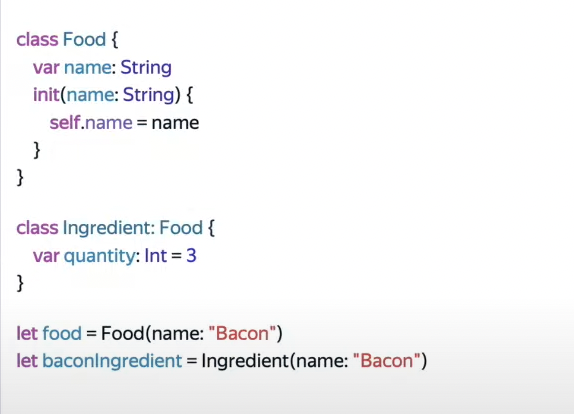
\includegraphics[scale = 0.5]{pic/classInitilizerSwiftAdv.png}
    \newline
    Второе правило говорит о том, что если подкласс определяет реализацию всех designated initilizer своего супер-класса, это можно сделать явно, с помощью слова \swift{@override} или, когда мы наследуем designated initlizer то автоматически наследуются все convinience initilizer супер-класса, посмотрим как это работает: 
    \newline
    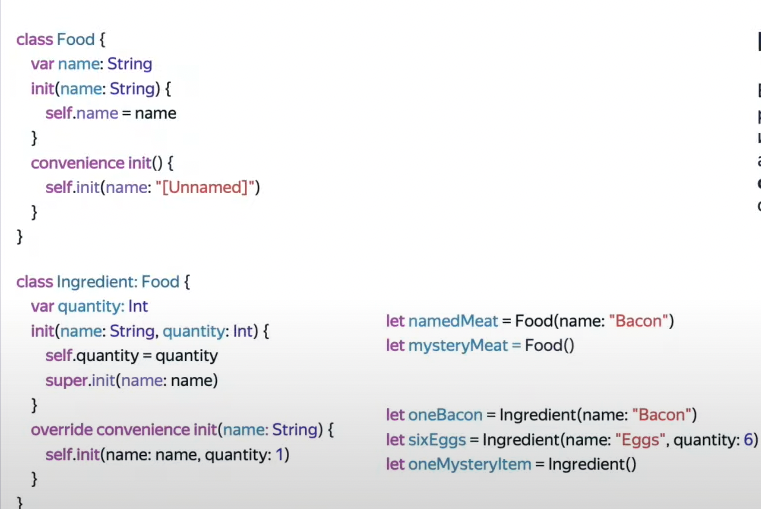
\includegraphics[scale = 0.5]{pic/FoodSwiftAdv.png}
    \newline
    Здесь у нас у класса food 2 инициализатора, один convinience, другой designated. У ingridient есть также 2 инициализатора. Сигнатура designated initlizer в классе ingridient соотвествует сигнатуре \textbf{designated initilizer} в классе food. Поэтому, даже не смотря на то, что в ingridient мы используем его как conviniense initilizer, мы должны писать ключевое слово \swift{@override}
    \newline
    Так как мы предоставили реализацию всех \swift{Designated initilizer}, то мы получили в подарок 1 \textbf{convinient initializer}
    \newline
    Что будет происходить, если мы вызовем ingridient без параметров? Мы вызовем convinience initilizer, который не принимает параметров, который наследуется от food, а затем вызовется convenience initilizer, а затем вызовется переопределенная реализация designated initilizer, то есть мы получим экземпляр класса ingridient с name = unnamed и quantiti = 1.
    \newline
    Иногда мы можем столкнуться с тем, что какой-то базовый класс при наследовании требует реализации какого-то инициализатора, очень явно можно с этим столкнуться, когда мы будет реализовывать наш \swift{UIViewController}. 
    \newline
    Это происходит из-за того, что есть ключевое слово \swift{required} и если мы пишем его к своему инициализатору, то все подклассы этого класса должны будут переопределеить этот инициализатор. 
    \newline
    При этом мы не пишем слово \swift{@override}, а также используем \swift{required}. 
    \newline
    Если мы не вводим в своем подклассе никаких инициализаторов, и при этом все хранимые свойства имеют значения по умолчанию, то мы наследуем этот инициализатор. 
    \newline
    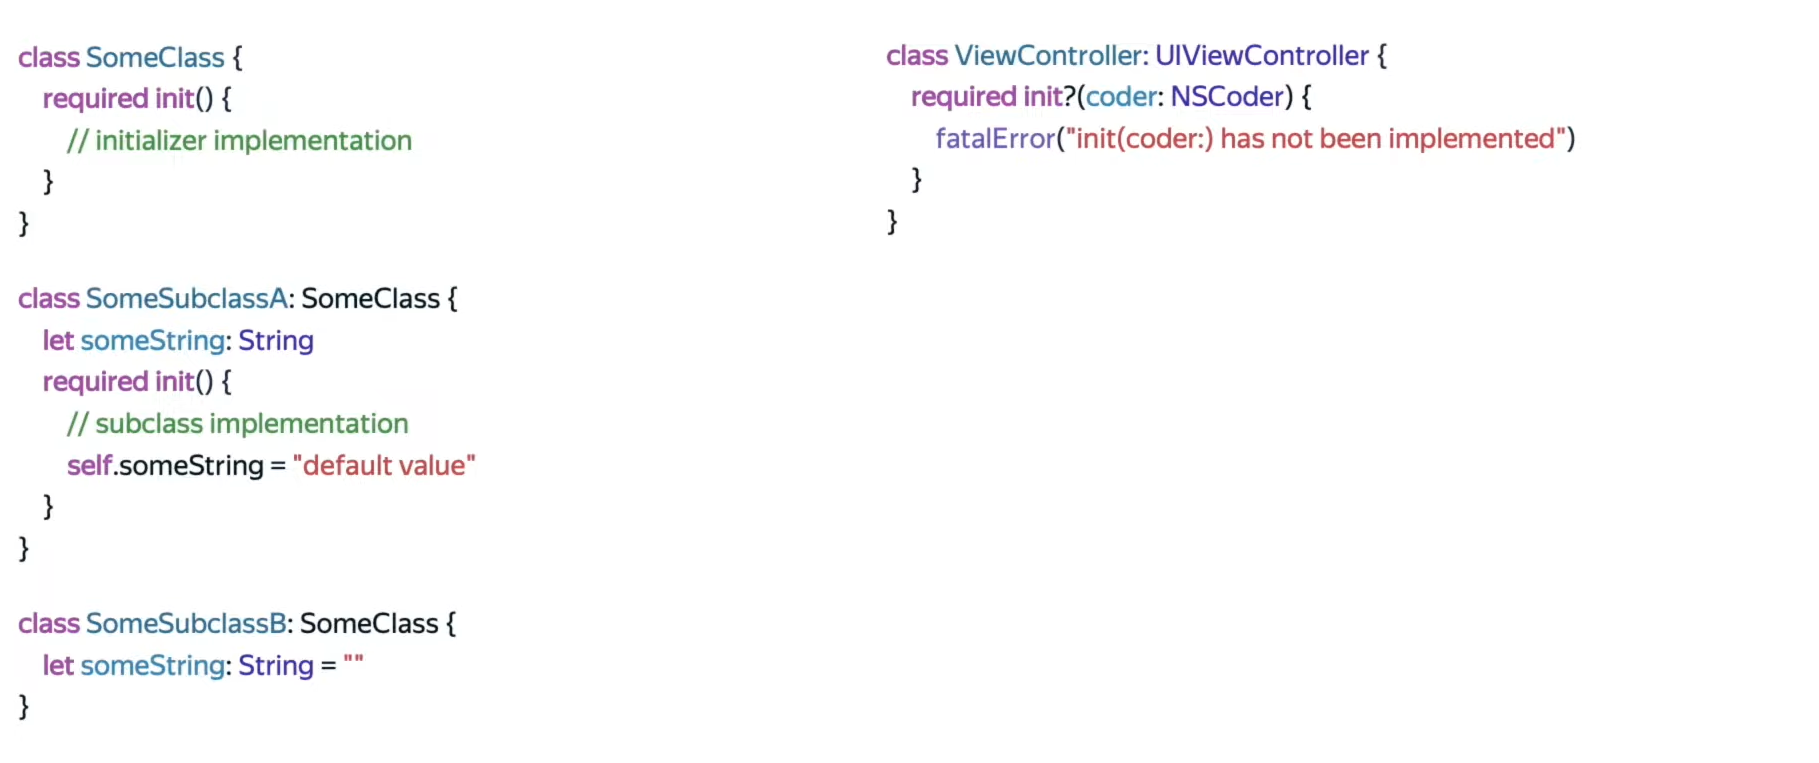
\includegraphics[scale = 0.2]{pic/requiredInitSwiftAdv.png}
    \newline
    Если мы захотим в таком случае реализовать свой инициализатор, то тогда нам потребуется реализовывать и все то, что указано с \swift{required}
    \subsection{ARC and retain cycle}
    У каждого reference type объекта есть счетчик ссылок, мы считаем количество ссылок на объект и когда это количество становится равным нулю, то объект уходит из памяти. 
    \newline
    Изначально в obj-c существовало ручное управление памятью, когда мы сами писали функции, которые напрямую влиют на этот счетчик ссылок, сейчас используется \textbf{ARC} -- автоматический подсчет ссылок. 
    \newline
    Функции, которые мы писали сами раньше, составляются за нас на этапе компиляции. Но при этом подсчет ссылок происходит в runtime
    \newline
    В swift есть 3 типа ссылок: 
    \begin{itemize}
        \item strong 
        \item weak
        \item unowned
    \end{itemize}
    Создадим такую ситуацию, когда объекты сами из памяти не уйдут, если не приложить никаких дополнительных усилий. Эта ситуация называется retain cycle. Рассмотрим как мы можем ее создать на примере: 
    \newline
    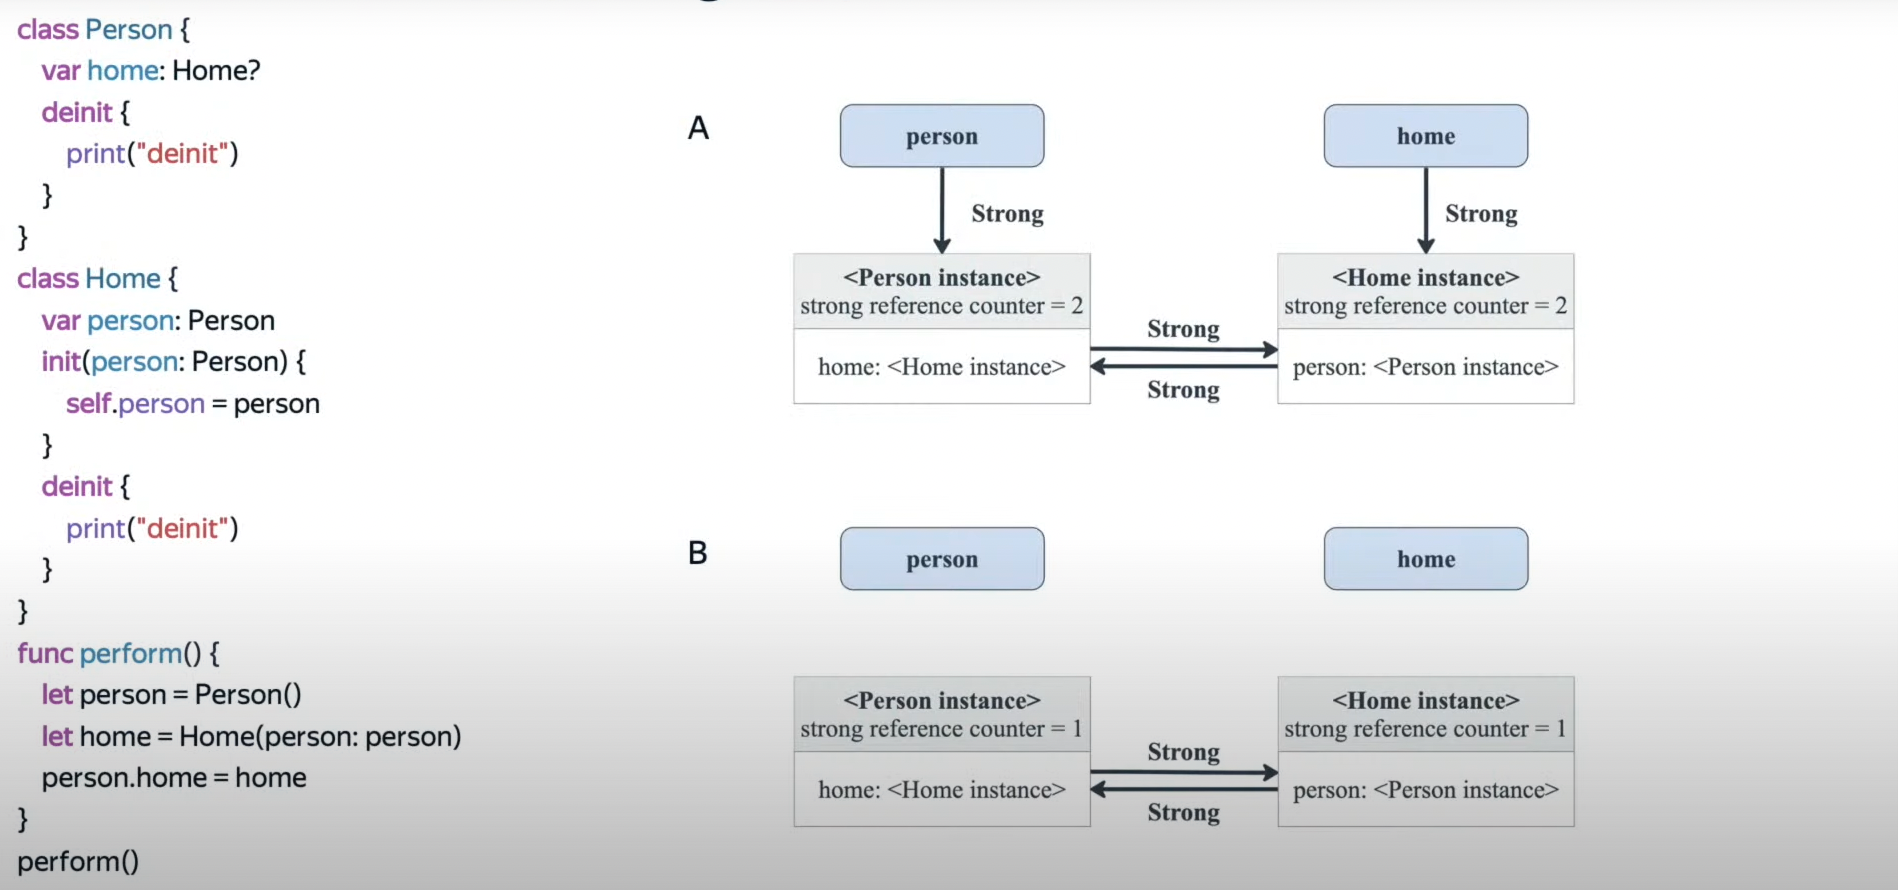
\includegraphics[scale = 0.2]{pic/arcSwiftAdv.png}
    \newline
    В методе perform мы создаем экземпляры классов, один из которых наследуется от другого, а при этом класс person ссылается на класс home.
    \newline
    Когда эта функция закончит свою работу, то эти переменные перестанут сильно держать person instance и home instance. 
    \newline
    Но при этом их счетчик сильных ссылок никогда не станет равным нулю, всегда 1, они не смогут уйти из памяти и произойдет утечка. Есть 2 выхода: использовать weak или unowned ссылки: 
    \subsubsection{Weak}
    Weak ссылки -- слабые ссылки и вводятся ключевым словом \swift{weak}, разрушают такой цикл засчет того, что не увеличивают ссчетчик сильных ссылок. 
    \newline
    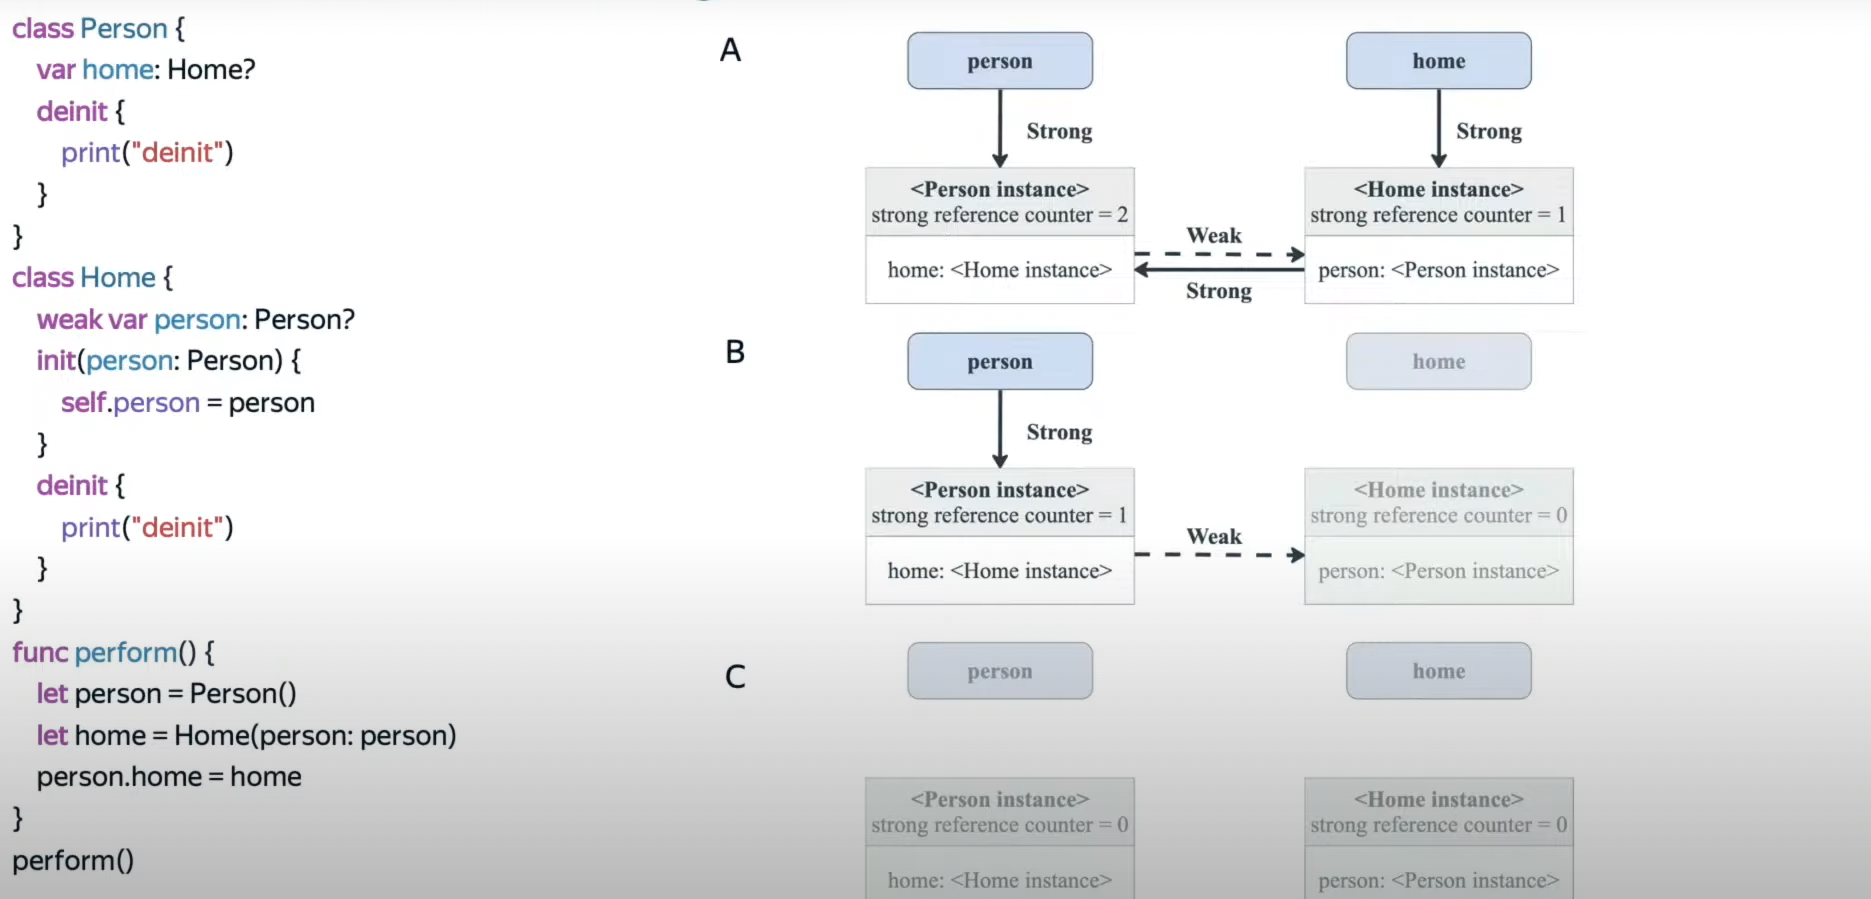
\includegraphics[scale = 0.2]{pic/weakCycleAdvSwift.png}
    \newline
    В данном случае в классе home мы сделали weak ссылку и получили схему на рисунке A. У weak ссылок есть механизм, который позволяет им обнулять ссылки в памяти, которые уже ушли из нее. 
    \newline
    В данном случае, если мы как на рисунке B обратимся по weak ссылке, то получим nil, поэтмоу weak ссылки должны быть var и опциональными. 
    \newline
    После того, как переменная person перестанет держать person instance оба объекта уйдут из памяти. 
    \newline
    \subsubsection{Unowned ссылки}
    В отличии от weak ссылок у них нет механизма, который будет их занулять, автоматически, если объект на который они указывают уйдет из памяти. 
    \newline
    Если мы обратимся к unowned ссылке, который ушел из памяти это приведет к runtime error, случится это может как на схеме B: 
    \newline
    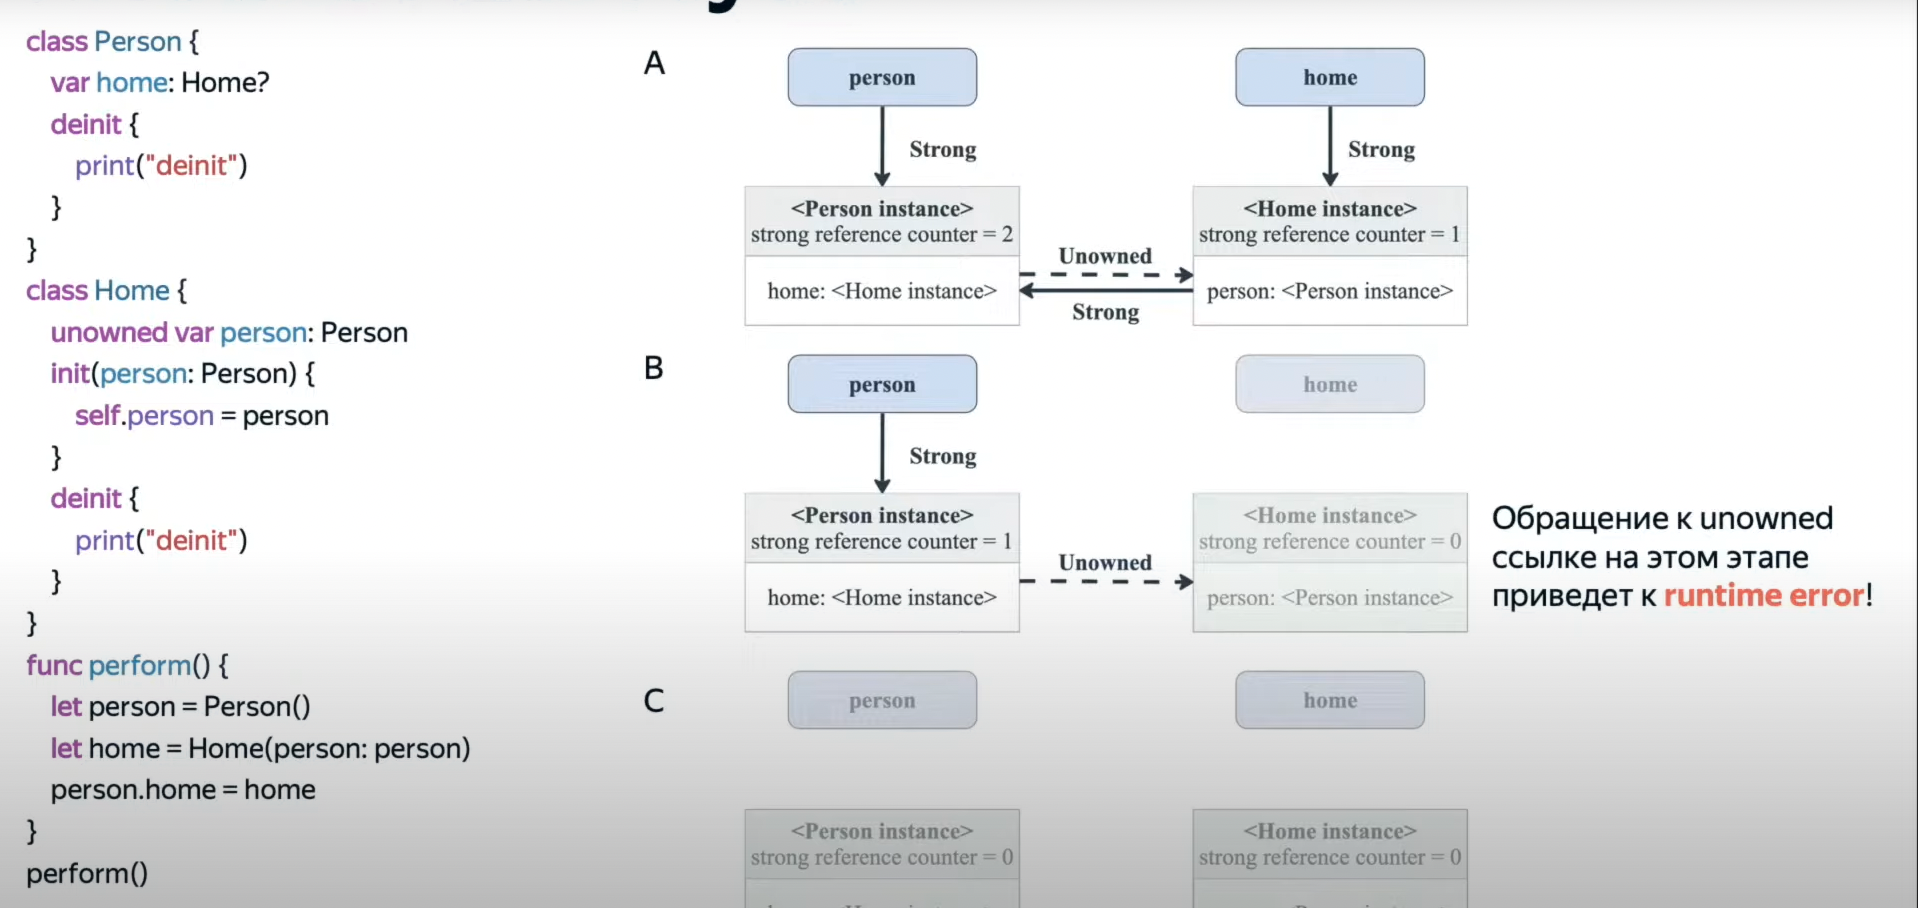
\includegraphics[scale = 0.2]{pic/unownedSwfitAdv.png}
    \subsection{Closures}
    Замыкание можно рассматривать, как анонимную функцию, которая из вне может в себя что-то захватывать
    \newline
    Они могут быть сохранены в переменные, переданы в другие функции и возвращены в функции. 
    \newline
    Замыкания могут захватывать переменные и константы из внешнего контектса двумя способами: неявно или яно, используя список захвата. 
    \newline
    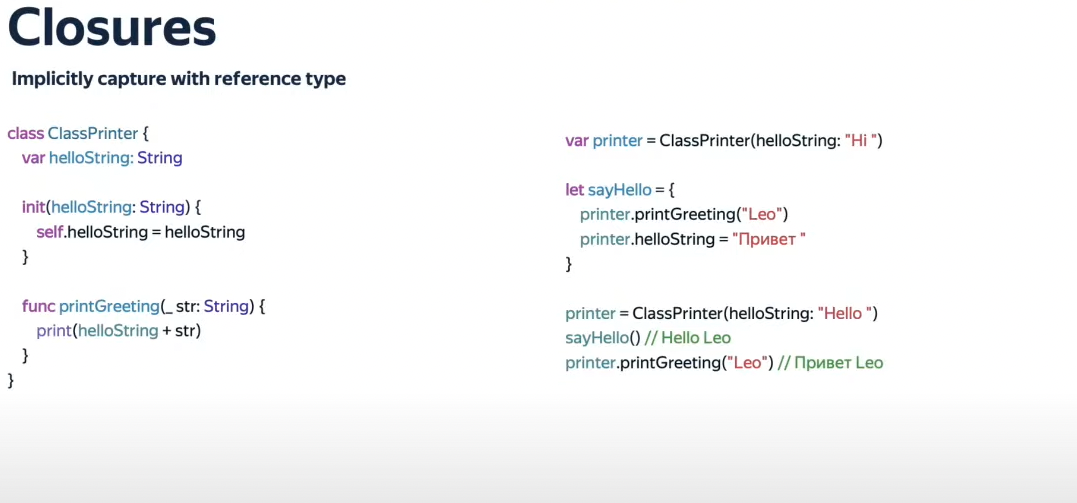
\includegraphics[scale = 0.2]{pic/clousersSwiftAdv.png}
    \newline
    Рассотрим неявный захват и то, как он работает с reference типами. 
    \newline
    Мы объявляем замыкание sayHello в котором мы неявно захватываем экземпляр класса \swift{Printer} и  принтим greetin и меняем helloString. Далее мы в принтер присваиваем другой экземпляр класса printer, когда мы захватываем неявно, то используем захват по ссылке, то есть захватываем на то, к чему присвоено имя printer. При вызове замыкания мы работаем уже с самым акутальным printer, поэтому получаем уже hello Leo. 
    \newline
    Когда мы работаем с value type и используем также неявный захват типов, то мы также захватываем и ссылку на этот объект и получаем точно такой же результат. 
    \newline
    Когда мы используем список захвата это можно рассмотреть, как передачу в качестве аргумента функцию. Потсмотрим как это выглядит на примере, начиная с reference типа. 
    \newline
    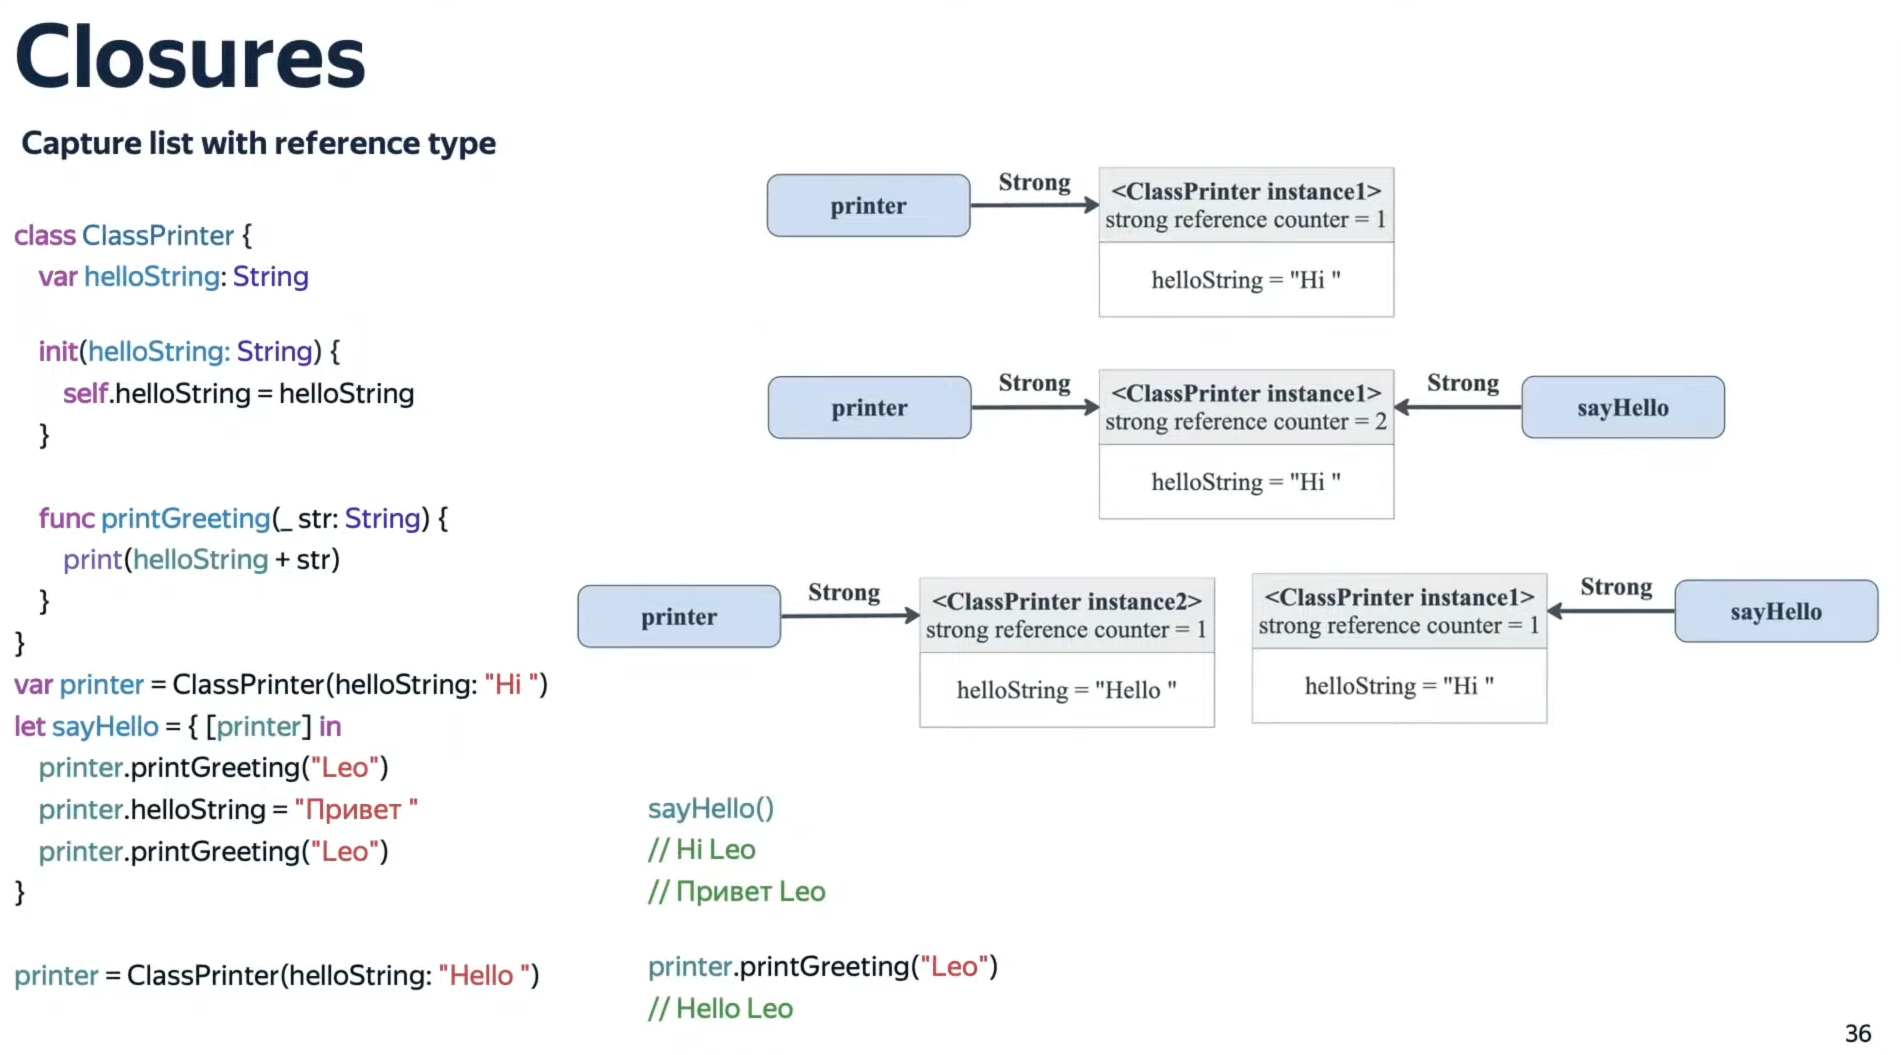
\includegraphics[scale = 0.2]{pic/ClosuerStrongAdvSwift.png}
    \newline
    Стоит отметить, что если бы в переменную printer мы бы не присваливали новый экзамепляр класса, а просто использовали поменяли бы константы в текущем, так как наше замыкание все еще ссылается на него, мы бы получили другой результат. 
    \newline
    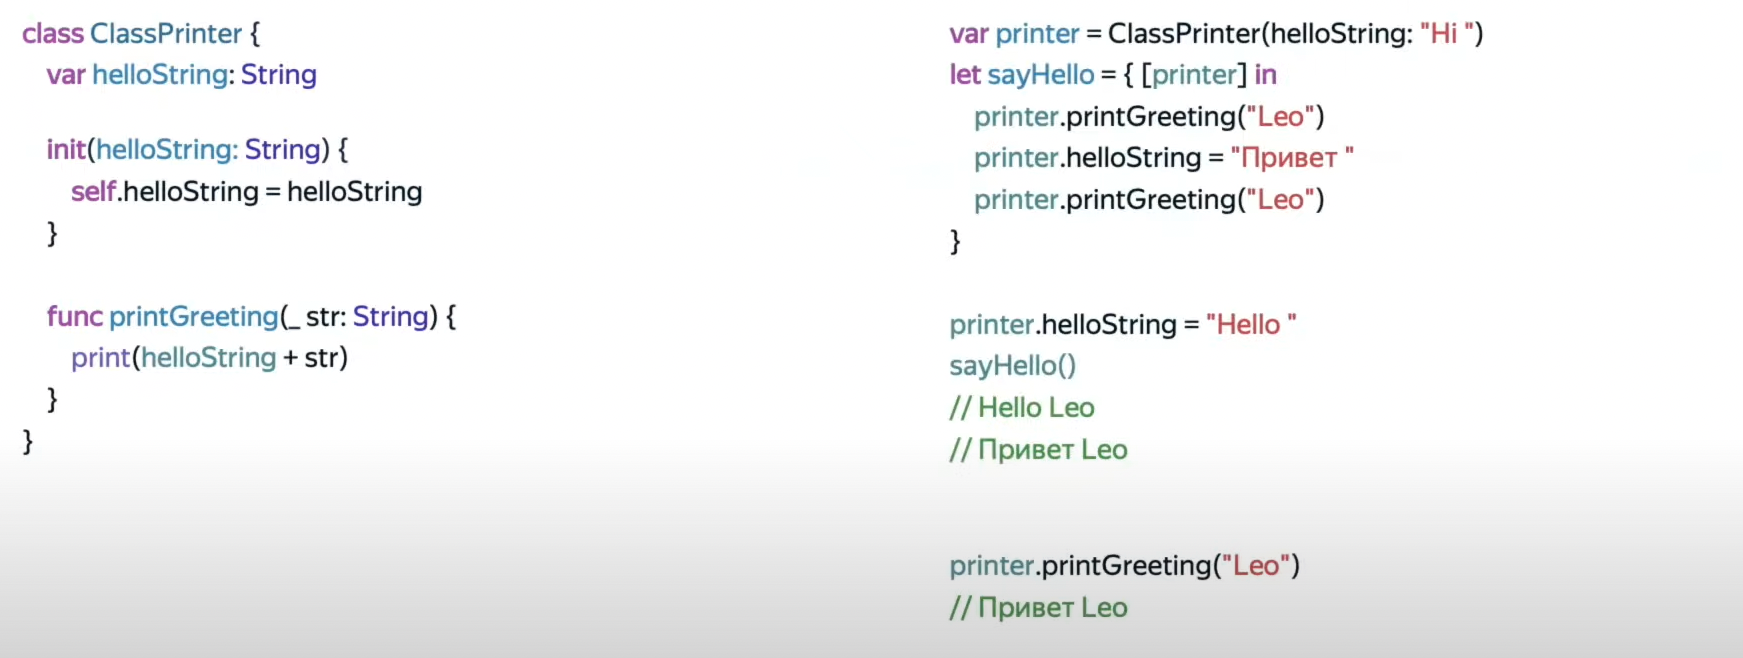
\includegraphics[scale = 0.2]{pic/closurePrinterRefTypeSwiftAdv.png}
    \newline
    Но в случае работе с value type мы будем копировать значение, которое было на момент замыкания, когда мы копируем это значение, оно будет доступно только для чтения и мы не сможем его менять.
    \newline
    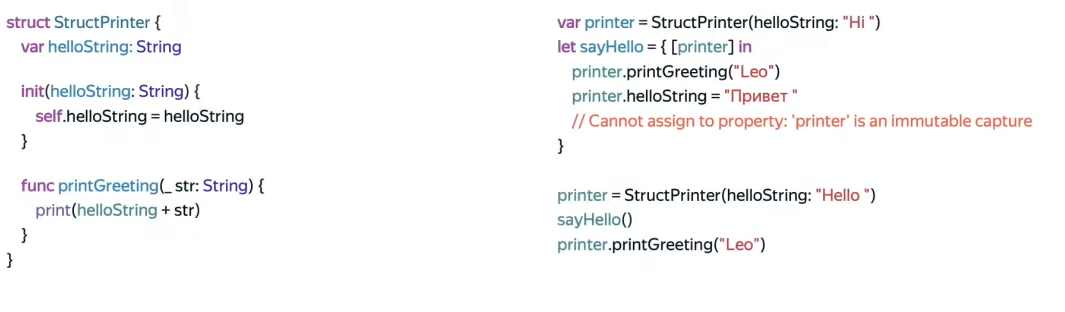
\includegraphics[scale = 0.4]{pic/closuerValueTypeSwiftAdv.png}
    \newline
    При захвате с reference типами мы можем также захватить как по weak так и по unowned ссылке, если ничего не дописывать, то мы будем работать с сильными ссылками. 
    \newline
    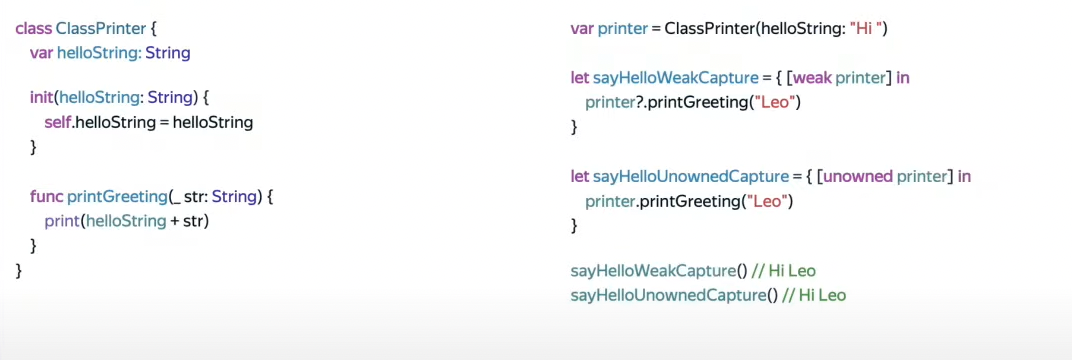
\includegraphics[scale = 0.4]{pic/Снимок экрана 2023-07-27 в 23.31.18.png}
    \newline
    Зачем нам это нужно? Замыкание это reference type, а следовательно мы можем случайно создать retain cycle, что не есть хорошо. Рассотрим на примере: 
    \newline
    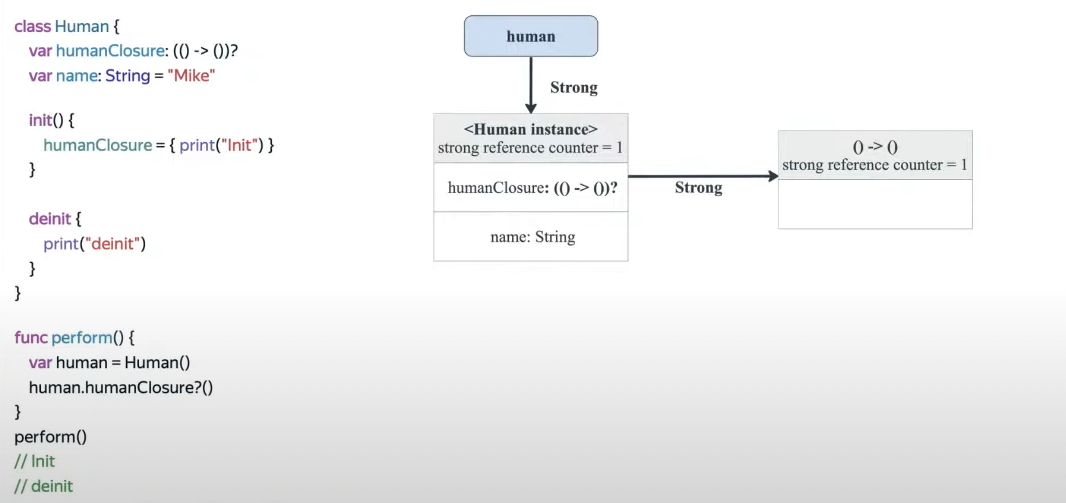
\includegraphics[scale = 0.5]{pic/Снимок экрана 2023-07-27 в 23.33.24.png}
    \newline
    У нас есть класс human, у него есть замыкание humanClosure. Напечатается все хорошо, но проблемы возникают далее: 
    \newline
    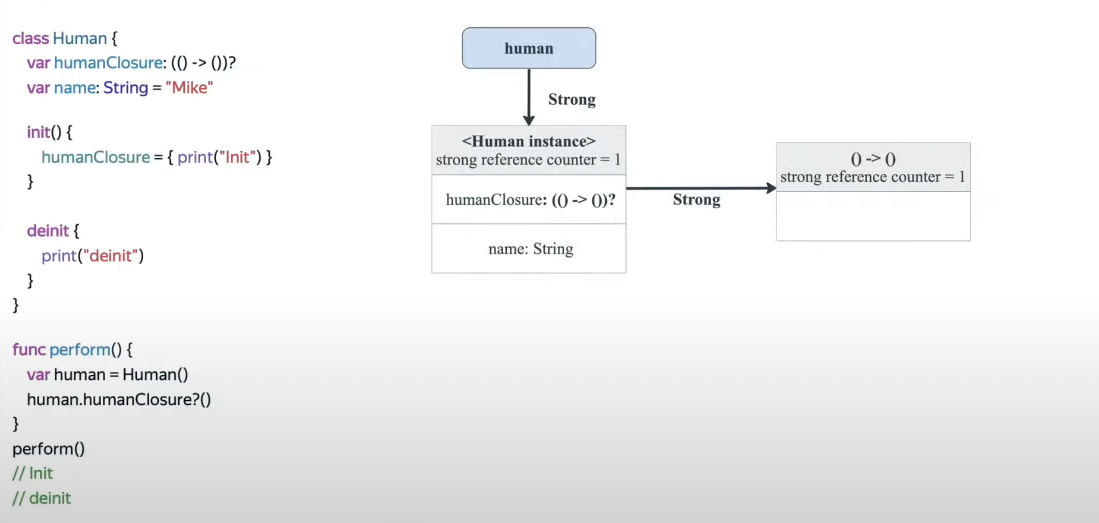
\includegraphics[scale = 0.5]{pic/Снимок экрана 2023-07-27 в 23.35.12.png}
    \newline
    В какой-то момент мы захотим напечатать init with и name, в эту секунду, когда мы так подумали, мы получили retain cycle, потому что мы захватили переменную не только переменную name, но и self и захватили по сильной ссылке. 
    \newline
    Когда perfom закончит свою работать, то перемнная human перестанет держать human instance, у них с замыканием все равно никогда счетчик ссылок не станет равным нулю. 
    \newline
    Решить эту проблему нам опять же помогут weak и unowned ссылки, которые мы можем использовать в списке захвата: 
    \newline
    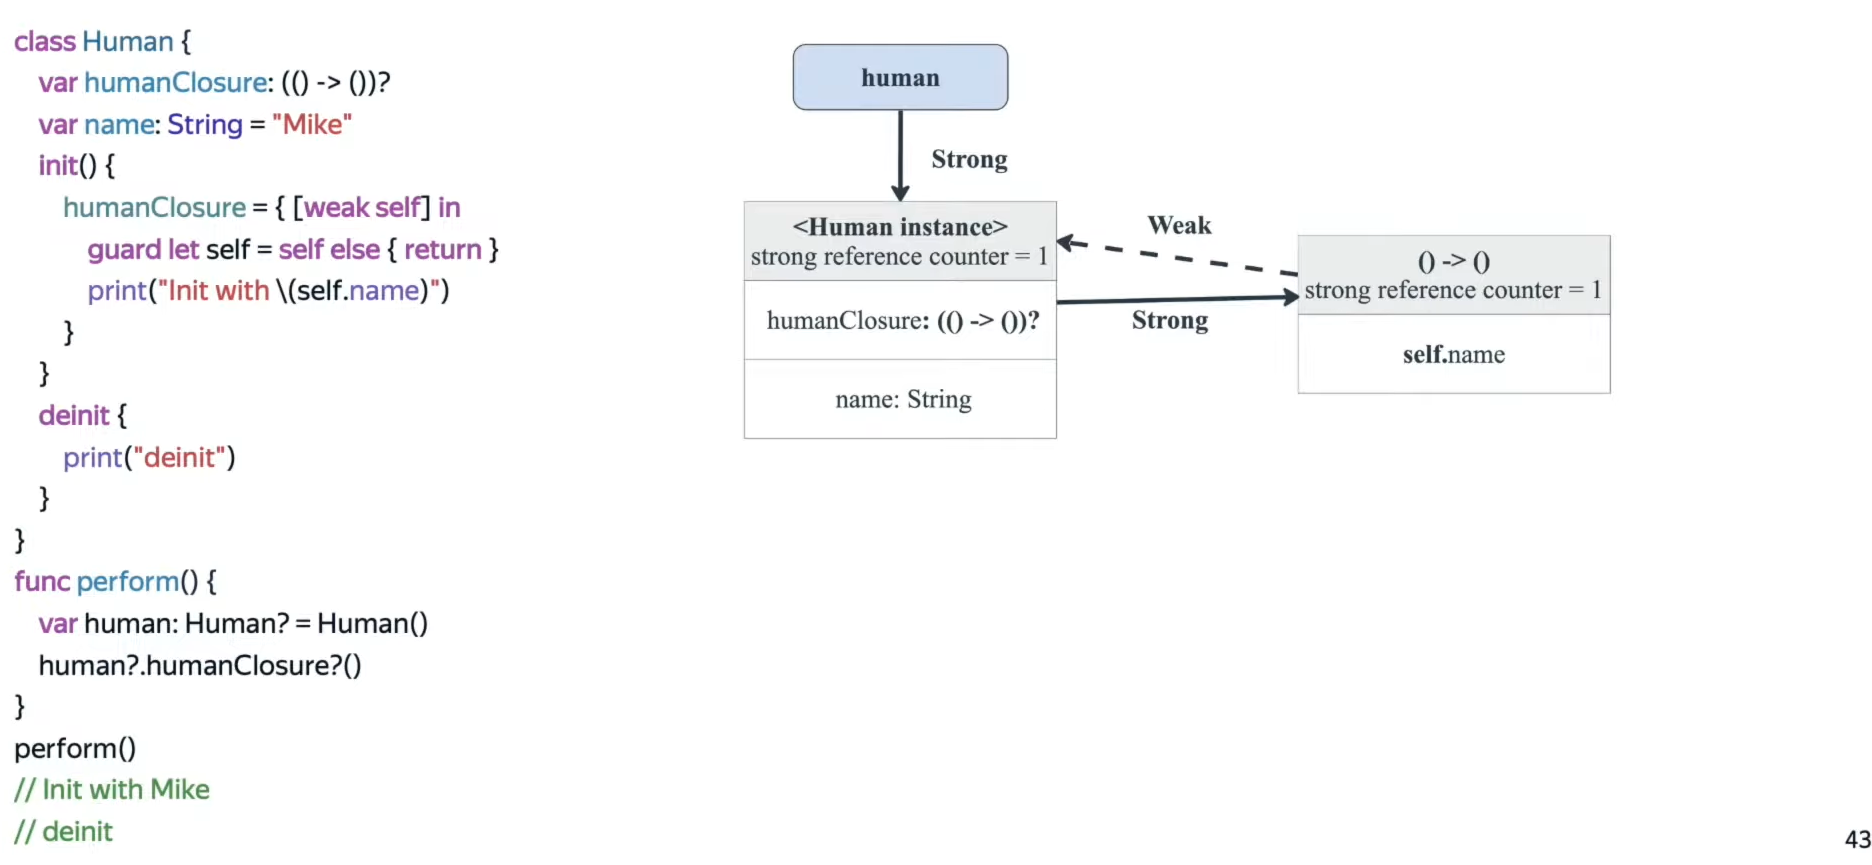
\includegraphics[scale = 0.3]{pic/Снимок экрана 2023-07-27 в 23.39.08.png}
    \newline
    Поговорим про ключевые слова
    \newline
    \swift{@autoclosure} -- заключает выражение, переданное как аргумент функции в тело замыкания. Рассотрим как это работает на примере: 
    \newline
    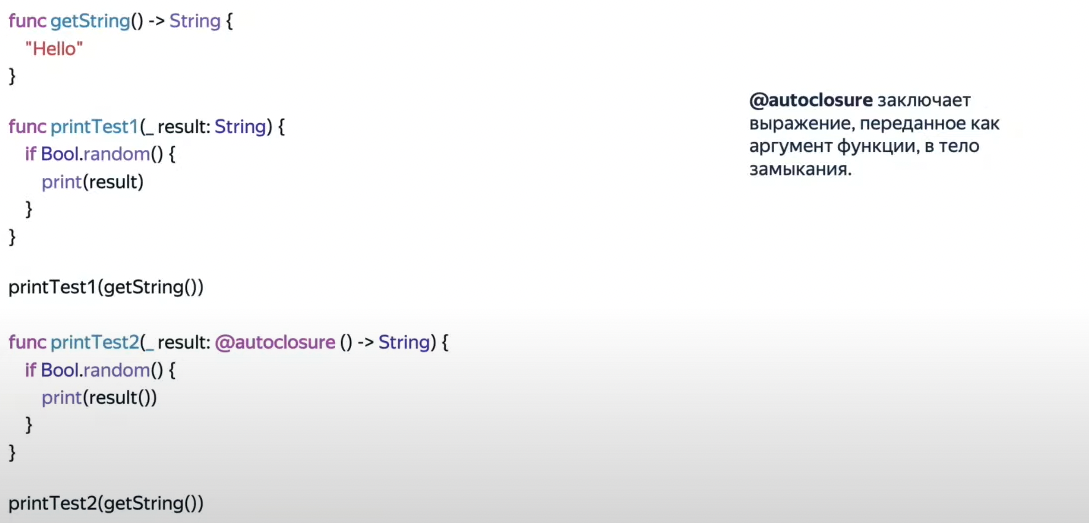
\includegraphics[scale = 0.5]{pic/Снимок экрана 2023-07-27 в 23.41.08.png}
    \newline
    \swift{@escaping} -- сообщает нам о том, что замыкание, которое мы передаем в качестве аргумента в фукнцию может пережить время действия этой функции. Сделать оно может это например, когда мы хотим передать замыакние в качестве аргумента и сохранить его потом в переменную и вызывать из нее. Такое мы не сможем сделать без нашего ключевого слова
    \newline
    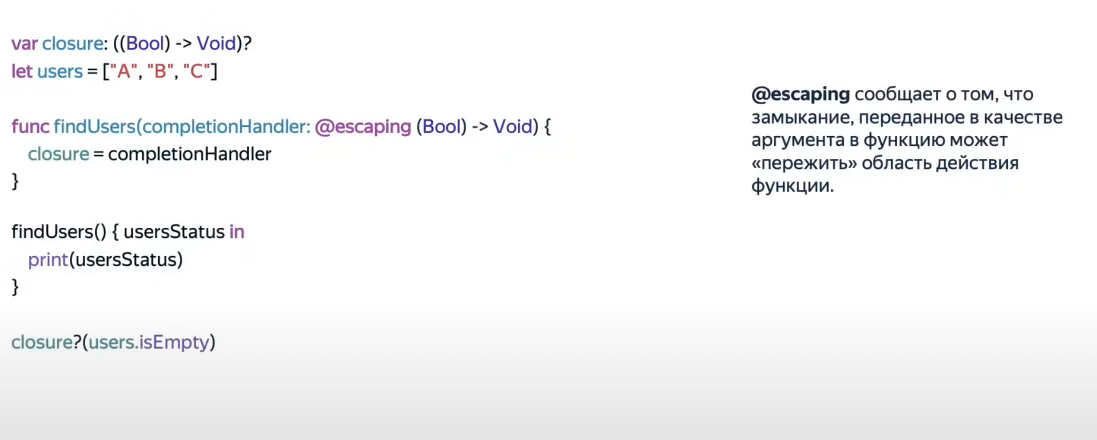
\includegraphics[scale = 0.5]{pic/Снимок экрана 2023-07-27 в 23.44.45.png}
    \newline
    \subsection{Protocols}
    В рамках протокола мы говорим о том, какие методы и свойства должны быть реализованы у класса, чтобы соотвествовать этому протоколу. 
    \newline
    В отличии от наследования протоколы могут поддерживать классы структуры и енамы и при этом могут соотвествовать неограниченному числу протоколов. 
    \newline
    В \textbf{Swift} протоколы могут содержать не только наименования методов и свойств, которые протоколы могут содержать, но и их реализацию в extention. Если мы такую реализацию пишем, то в классе который соотвествует этому протоколу мы можем не реализовывать эти методы или свойства, они будут нам доступны из расширения протокола: 
    \newline
    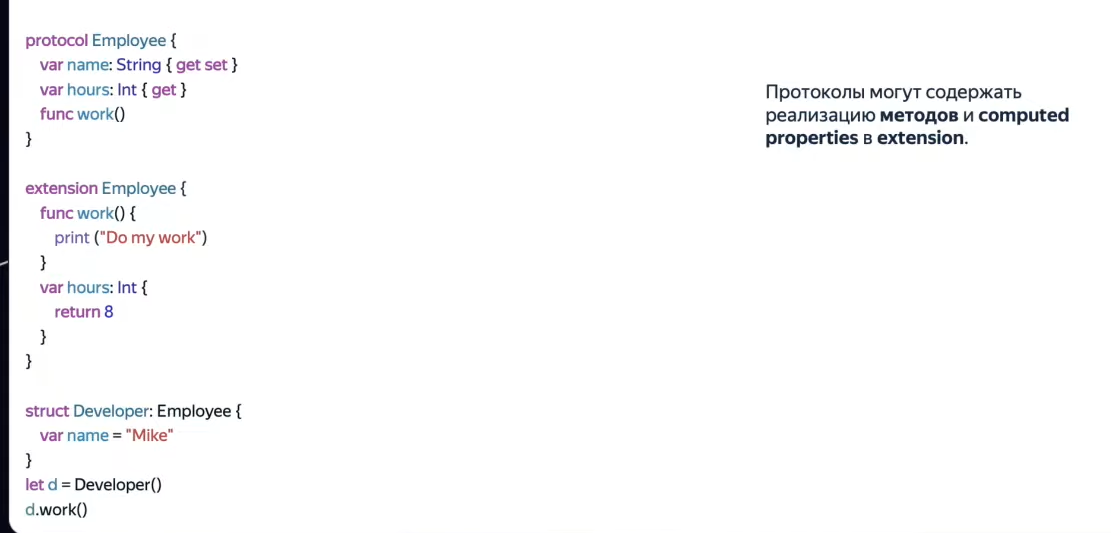
\includegraphics[scale = 0.5]{pic/Снимок экрана 2023-07-27 в 23.48.50.png}
    \newline
    Swift поддерживает иерархию протоколов: 
    \newline
    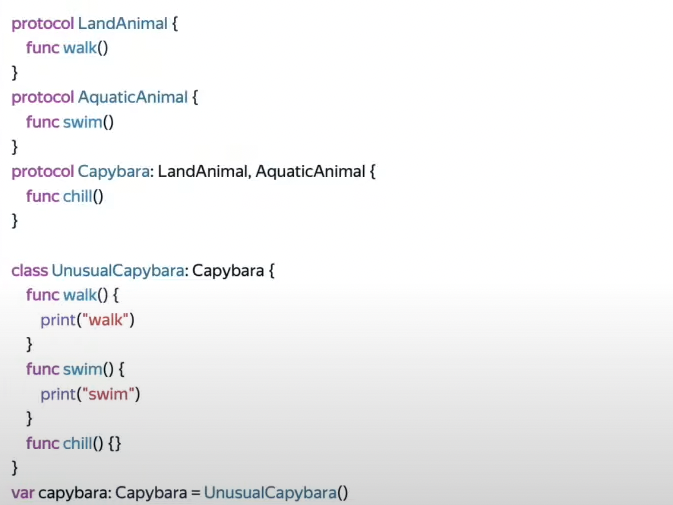
\includegraphics[scale = 0.5]{pic/Снимок экрана 2023-07-27 в 23.49.39.png}
    \newline
    Это не то же самое, что и наследование классов. Когда мы говорим про протоколы, мы говорим что те, кто соотвествуют протоколу Capybara также должны соответсвовать протоколу LandAnimal и AquaticAnimal.
    \newline
    Также есть композиция протоколов: \swift{var capybara1:LandAnimal & AquaticAnimal = UnusualCapybara}
    \newline
    Мы можем эту композицию захотеть использовать в качестве типа. Это не создает новый тип, но мы можем захотеть работать с типом, который соответсвует одновременно LandAnimal и AquaticAnimal. Такая запись длинная и неудобная, поэтому используются \swift{typealias}, который просто заменяет длинную запись, не создавая при этом новый тип. 
    \newline
    Если мы хотим, чтобы протоколам могли соответсоввать только классы для этого мы используем наследование от специального протокола AnyObject. Это тот протокол, которому неявно соответствуют все классы. 
    \newline
    Зачем нам может это захотеться? Рассмотрим наш пример, на котором мы рассматривали наш retain Cycle. 
    \newline
    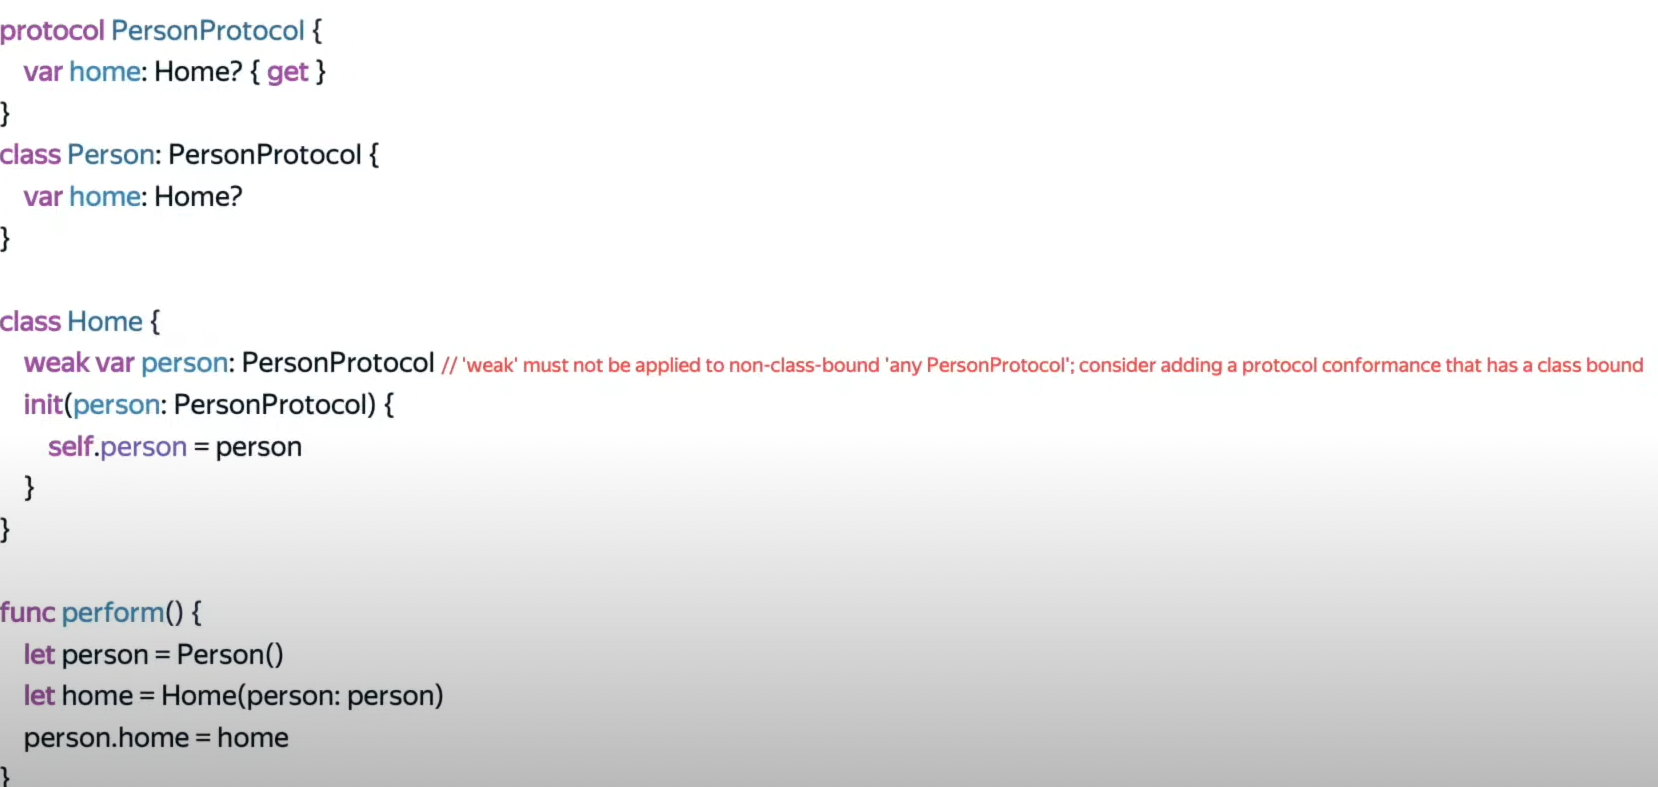
\includegraphics[scale = 0.5]{pic/Снимок экрана 2023-07-28 в 00.00.15.png}
    \newline
    Например здесь weak может относится только к reference типам, при этом если у нас протокол PersonProtocol не наследует AnyObject у нас может быть и value type. Поэтому компилятор выдаст ошибку. 
    \newline
    Если мы ограничиваем протокол так, чтобы ему соотвествовали только классы нам становится доступная возможность писать weak.
    \subsection{Method dispatch}
    Диспетчеризация -- процесс поиска реализации вызываемого метода, проихсодит каждый раз, когда мы у нашего объекта вызываем какой-то метод. Бывает трех типов: \textbf{Direct Dispatch, Table Dispatch(состоит из Virtual Table Dispatch и Witness Table Dispatch), Message Dispatch}
    \subsubsection{Direct Dispatch}
    Самый быстрый тип диспетчеризации, также называют статической диспетчеризацией. По сути это вызов метода, когда на этапе компиляции мы знаем, что в этом месте будет вызвана вот эта конкретная реализация. У всех \textbf{value type} по умолчанию используется Direct Dispatch, так как мы не можем их поменять, переопределить. 
    \newline
    Не поддерживает полиморфизм и наследование. 
    \newline
    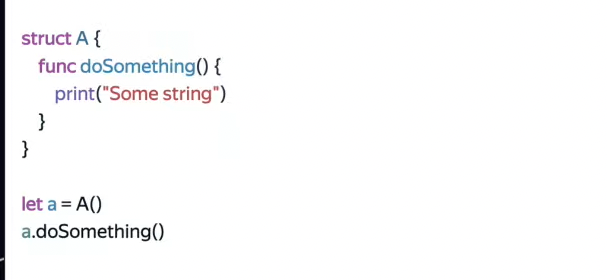
\includegraphics[scale = 0.5]{pic/Снимок экрана 2023-07-28 в 19.07.42.png}
    \newline
    Когда еще мы можем иметь дело с Direct Dispatch? Когда мы добавляем слово \swift{final} в объявлении класса, то у этого класса не могут создаваться классы наследники и наследование для этого класса становится недоступным, соответвенно мы не можем в классе наследнике переопределить методы, которые мы там объявляем, поэтому их диспетчеризация меняется на статическую.
    \newline
    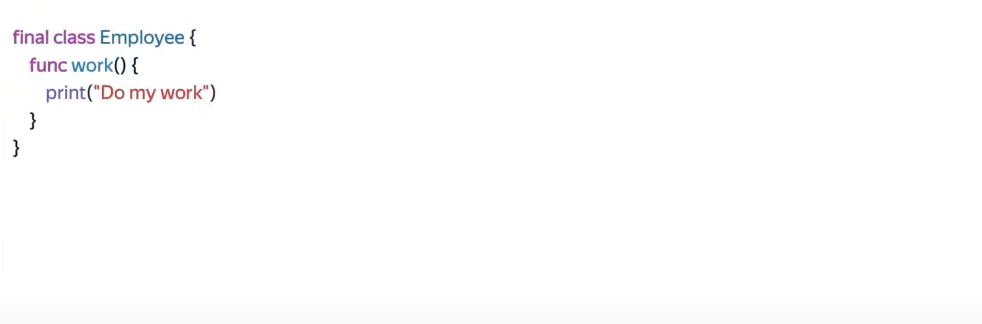
\includegraphics[scale = 0.5]{pic/Снимок экрана 2023-07-28 в 19.10.18.png}
    \newline
    Если мы объявляем метод в расширении протокола, и при этом в протоколе, в описании его не добавляем, то для этого метода также диспетчеризация становится статической: 
    \newline
    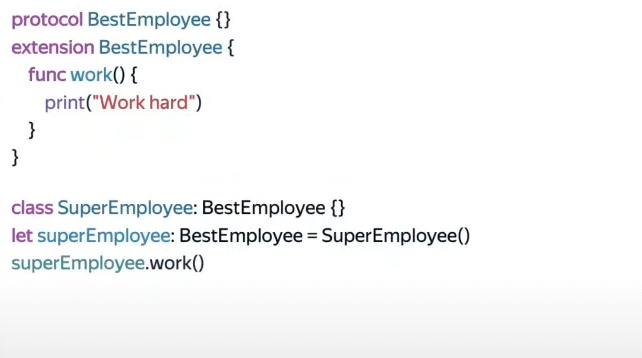
\includegraphics[scale = 0.5]{pic/Снимок экрана 2023-07-28 в 19.12.04.png}
    \newline
    Если мы объявляем метод в расширении протокола, и при этом в протоколе, в описании его не добавляем, то для этого метода также диспетчеризация становится статической. 
    \newline
    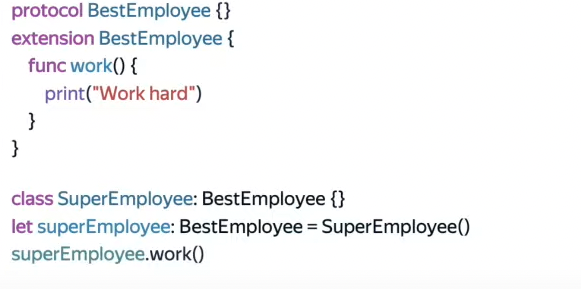
\includegraphics[scale = 0.5]{pic/Снимок экрана 2023-07-28 в 19.13.09.png}
    \newline
    Когда мы пишем класс и добавляем методы в его расширении, то мы можем использовать их из класса наследника, но мы не можем их переопределить, и диспатчеризация становится для них статической. 
    \newline
    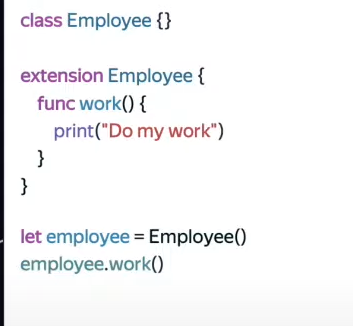
\includegraphics[scale = 0.5]{pic/Снимок экрана 2023-07-28 в 19.14.41.png}
    \newline
    Когда мы пишем \swift{private} к методу в классе, то его диспатчеризация также переходит на статическую, потому что мы его не сможем не использовать не переопределить из класса наследника. 
    \subsubsection{Virtual Table Dispatch}
    Используется при наследовании классов, создается на этапе компиляции(Virtual table), для каждого класса и его подкласса. 
    \newline
    Рассмотрим как это работает на примере: 
    \newline
    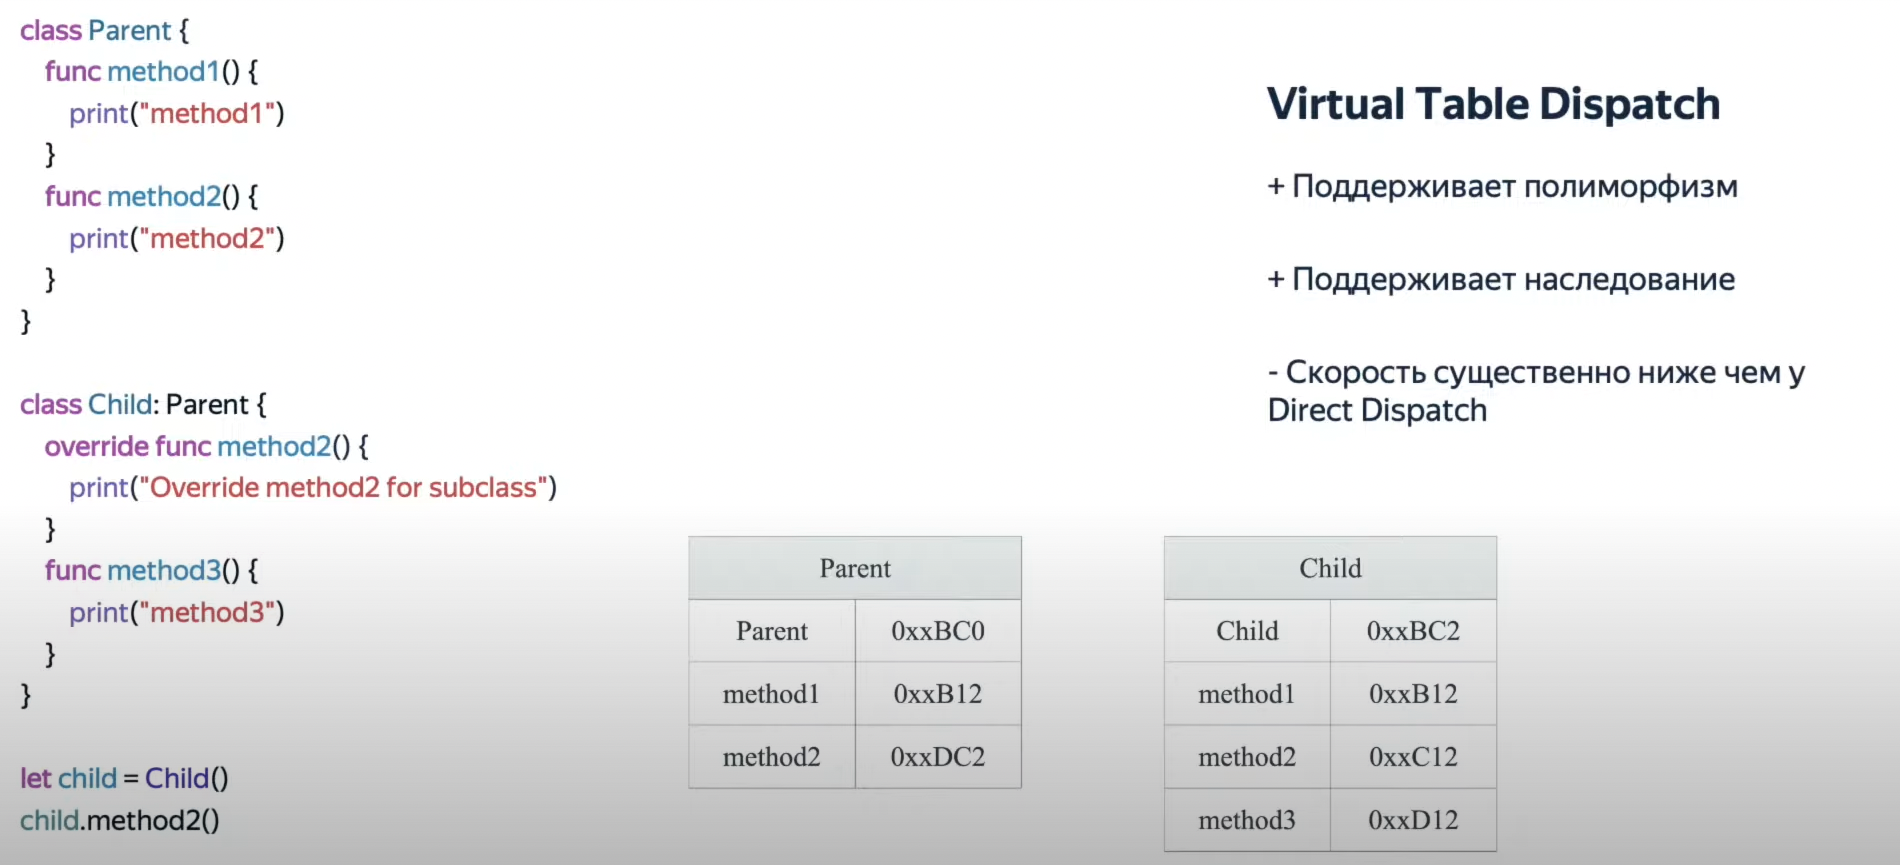
\includegraphics[scale = 0.2]{pic/Снимок экрана 2023-07-28 в 19.16.57.png}
    \newline
    Мы переопределили метод 2 в подклассе, и ввели новый метод 3. На этапе компиляции у нас создасться Virtual Table для класса родителя, у него есть методы и указатель на их реализацию.
    \newline
    Для класса наследника мы копируем Virtual table родителя. method1 мы в классе наследнике не переопределили, поэтому в Virtual Table для класса наследника он указывает туда же, куда указывает Virtual Table для класса родителя. Method2 мы переопределили и у него поменялся указатель. Также мы добавили новый method3, что отобразилось в Virtual Table для подкласса. 
    \newline
    Когда мы создаем экземпляр класса \swift{Child}, то на этапе компиляции создаются Virtual Table, а в Runtime мы идем в соотвествующую таблицу и ищем, где находится реализация соотвествующего метода, чтобы ее вызвать. 
    \subsubsection{Witness table Dispatch}
    Используется для реализации протоколов, например:
    \newline
    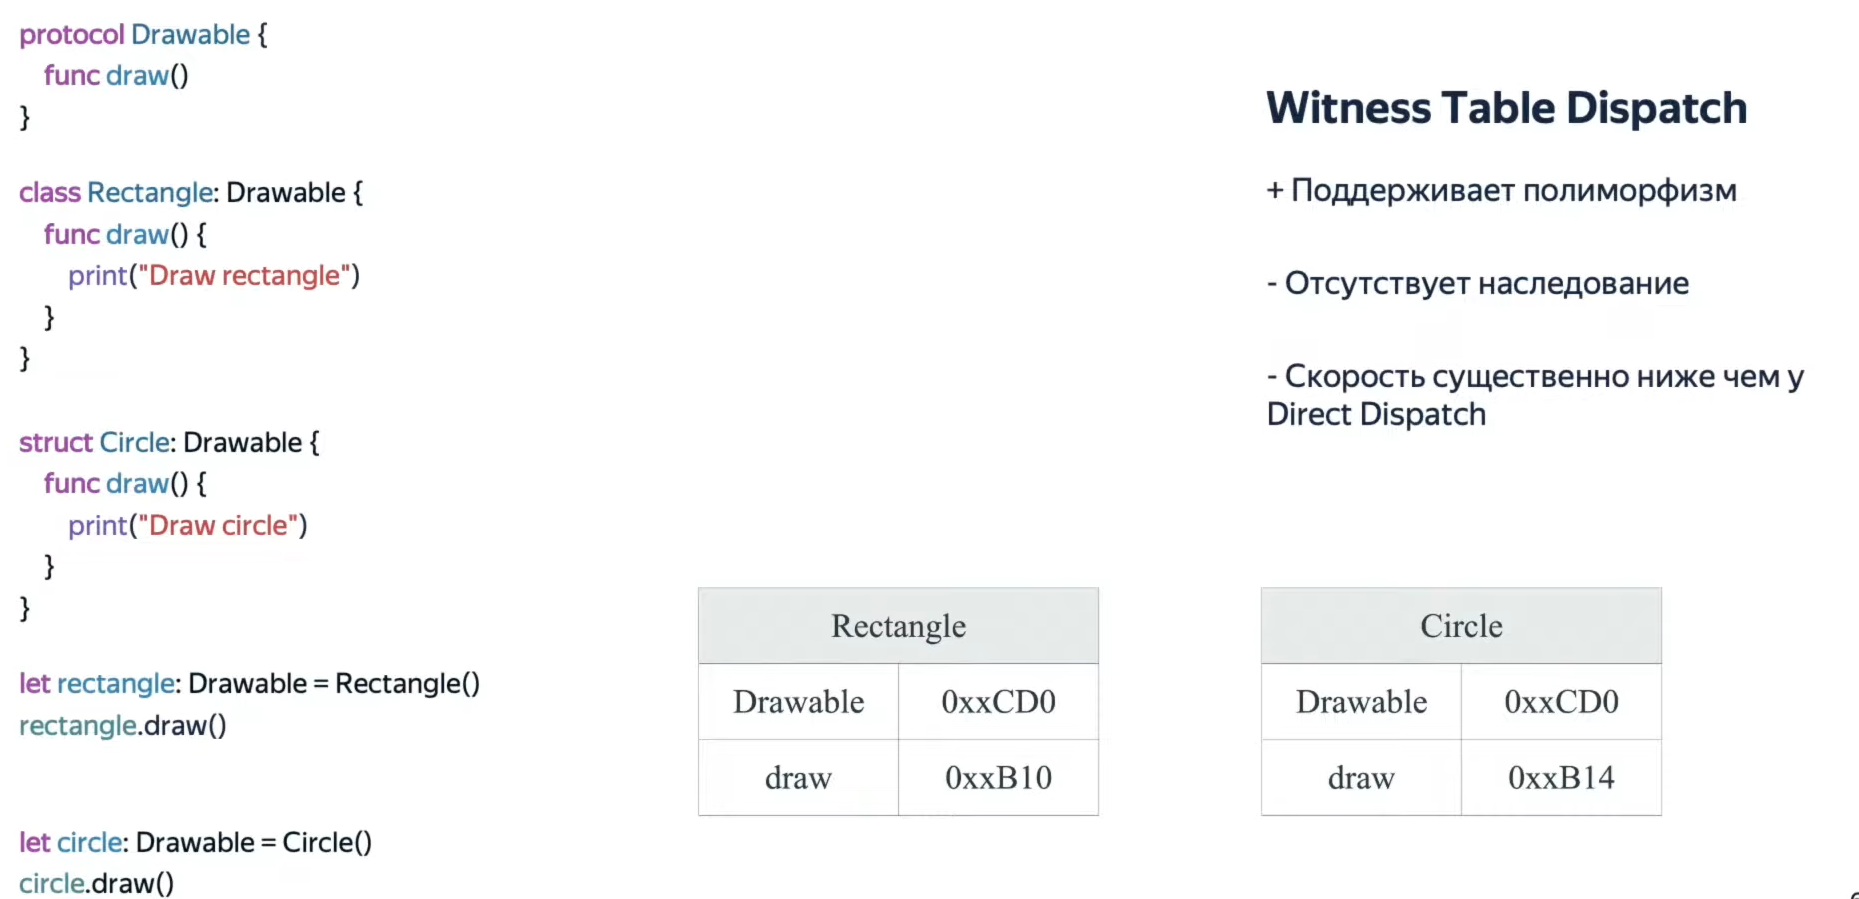
\includegraphics[scale = 0.2]{pic/Снимок экрана 2023-07-28 в 19.26.31.png}
    \newline
    У нас есть класс и структура, которые соотвествуют этому протоколу. Witness table создается на этапе компиляции для тех типов, которые соответсвуют этому протоколу. В данном случае создаются Witness table, у них есть указатель на сам протокол и на реализацию метода. 
    \newline
    Если мы создаем переменную типа протокола, и при этом она будет объектом класса. Во время выполнения метода такой переменной мы пойдем в Witness table и будем искать его реализацию. Происходит Witness table dispatch. Такой подход поддерживает полиморфизм, но не поддерживает наследование. Поскольку и для Virtual table и для Witness table dispatch во время выполнения ходим в таблицы и ищем в них методы их скорость существенно ниже чем у Direct Dispatch.
    \subsubsection{Message Dispatch}
    Самый динамичный тип диспатчеризации, обычно используется в связке с obj-c. Полностью работает в runtime, рассмотрим пример: 
    \newline
    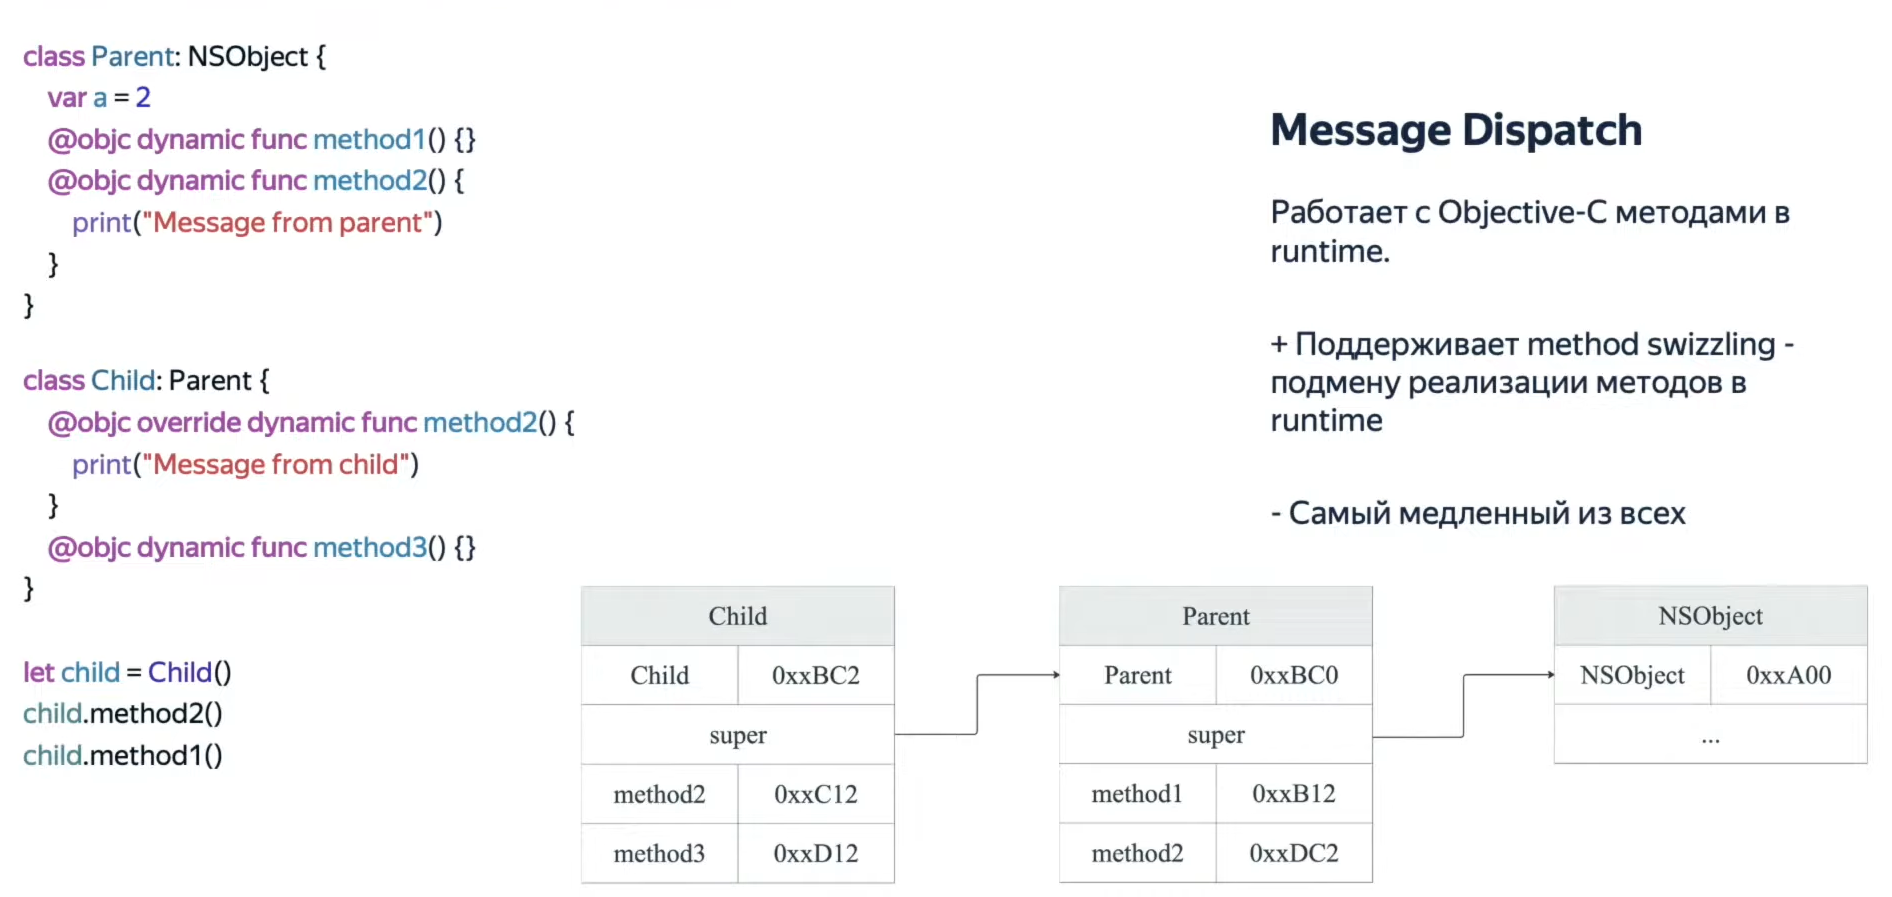
\includegraphics[scale = 0.2]{pic/Снимок экрана 2023-07-28 в 19.33.48.png}
    \newline
    Для того, чтобы указать, что для метода мы хотим использовать message Dispatch необходимо использовать слово \swift{Dynamic}. Также для того, чтобы метод стал виден в obj-c runtime необходимо использовать тег \swift{objc}.
    \newline
    Поскольку это все работает в runtime, на этапе компиляции никакие таблицы не создаются. У нас также есть таблица для \textbf{Child} и для \swift{Parent}, но при этом таблица \swift{Child} уже не копируется из таблицы \swift{Parent}. 
    \newline
    Например мы у child вызываем method2, идем в таблицы child, ищем реализацию method2 и ее вызываем. Если мы вызываем method1, который мы не переопределили, идем в таблицу, видим, что этого метода нет, тогда с помощью super идем в таблицу, для класса родителя и ищем метод так. Мы ищем метод рекурсивно у классов родителей, пока его не найдем. 
    \newline
    Метод является самым медленным из всех, так как работает в runtime. Но поддерживает method swizzling -- подмену реализации методов в runtime. 
    \subsubsection{Тонкости диспатчеризации}
    Рассмотрим пример:
    \newline
    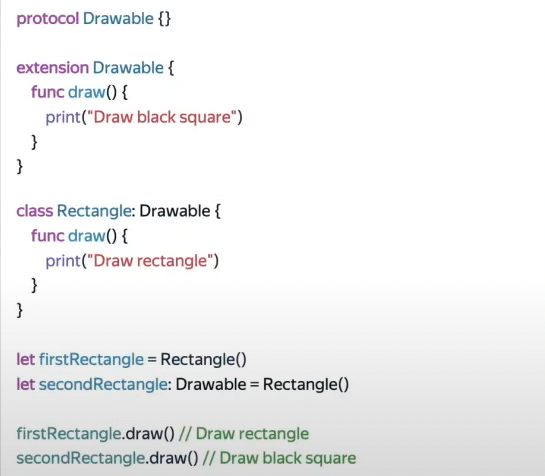
\includegraphics[scale = 0.5]{pic/Снимок экрана 2023-07-28 в 19.41.49.png}
    \newline
    Метод Drawable мы добавили в Extension, поэтому для него диспатчеризация будет статической. 
    \newline
    firstRectangle является переменной типа Rectangle, тогда как secondRectangle является переменной Drawable. 
    \newline
    у secondRectangle при вызове метода draw вызывается реализация из extension, как раз таки потому, что мы поменяли диспатчеризацию на статическую. 
    \newline
    Если мы не хотим такого поведения нужно не забывать добавить этот метод в описание протокола. В таком случае мы получим Witness Table Dispatch и при вызове метода draw(), вызовем реализацию из класса. 
    \newline
    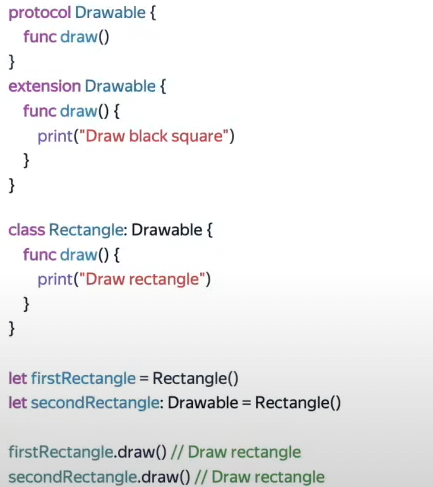
\includegraphics[scale = 0.5]{pic/Снимок экрана 2023-07-28 в 19.47.19.png}
    \newline
    Также в swift есть некоторое неочевидное поведение: 
    \newline
    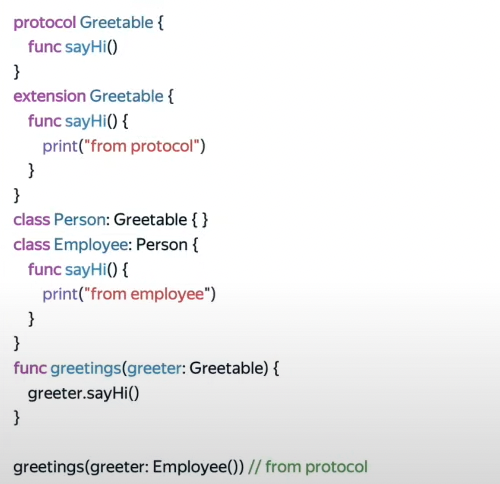
\includegraphics[scale = 0.2]{pic/Снимок экрана 2023-07-28 в 19.52.22.png}
    \newline
    В чем оно заключается? Оно гласит, что defaultная реализация метода из расширения протокола не может быть переопределена под классом. 
    \newline
    В Person нас устраивала реализация из протокола, а в наследнике мы решили переопределить метод. 
    \newline
    Если в greeting мы отправляем экземпляр класса \swift{Employer}, то все равно при вызове \swift{.sayHi} мы получим реализацию из протокола. 
    \newline
    Все потому, что деволтная реализация метода из расширения протокола не может быть переопределена подклассом
    \newline
    Если мы не хотим такого поведения, надо в классе, которые изначально соотвествует протоколу добавить реализацию этого метода. Если это сделать, то тогда мы получим реализацию уже из класса наследника. 
    \newline
    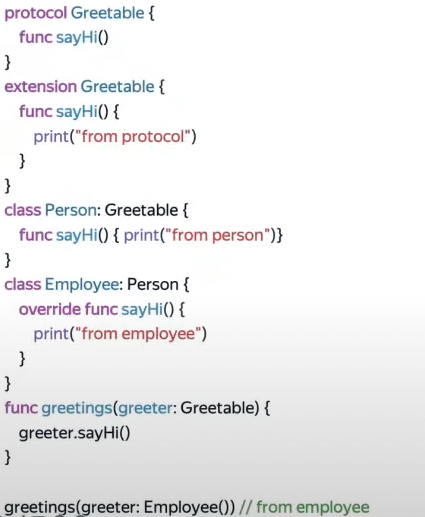
\includegraphics[scale = 0.5]{pic/Снимок экрана 2023-07-28 в 20.00.43.png}
    \newline
    Нужно быть внимательными с методами из расширения протокола и подумать о том, не захотим ли мы где нибудь в каком-нибудь классе насленике их переопределить. 
    \subsection{Generics}
    Представим, что нам нужно сделать какую-то функцию, которая складывает сумму двух элементов, мы знаем, что мы работаем с типами \swift{int} и \swift{double}
    \newline
    Мы можем написать 2 перегрузки функции sum, просто с разными параметрами. 
    \newline
    Заметим, что реализация у них будет совершенно одинаковая. 
    \newline
    А что если в такую функцию мы можем передать не 2 типа, а 10, 15 или 20? Каждый раз писать новую функцию -- кринж. 
    \newline
    На помощь приходят дженерики, мы можем написать функцию, которая может принимать любой тип, например сумма будет выглядеть так: 
    \newline
    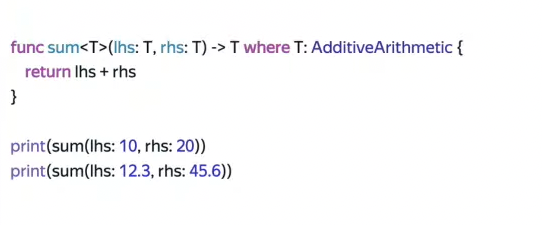
\includegraphics[scale = 0.5]{pic/Снимок экрана 2023-07-28 в 22.32.50.png}
    \newline
    Тип с которым мы будем работать в данном случае будет вычеслен исходя из аргументов, которые мы передаем в нашу функцию. 
    \newline
    Когда мы работаем с такими функциями операторы и методы которые мы используем(у типа Т в данном случае) должны быть на нем определены, как раз это и достигается ограничением протоколом. 
    \newline
    Мы также можем использовать Generics и их ограничение протоколом для структур, enum и классов: 
    \newline
    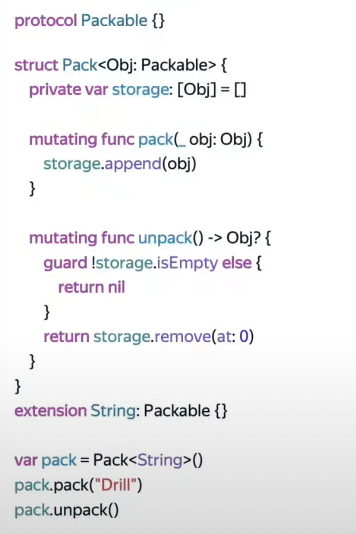
\includegraphics[scale = 0.5]{pic/Снимок экрана 2023-07-28 в 22.35.56.png}
    \newline
    Когда мы создаем экземпляр такого класса мы должны явно указать какому типу будет соответстсововать generic тип. 
    \newline
    Протоколы могут также использовать generic, для этого используется ключевое слово \swift{associatedtype}
    \newline
    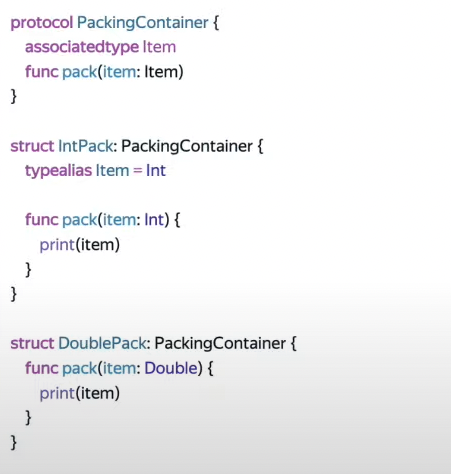
\includegraphics[scale = 0.5]{pic/Снимок экрана 2023-07-28 в 22.37.32.png}
    \newline
    Когда тип соотвествует такому протоколу, то необходимо либо явно, через \swift{typealias} указать, какому типу будет соответсововать наше введенное название, либо этот тип будет вычеслен исходя из тех реализаций, которые мы предоставляем. 
    \newline
    Внутри определения протокола или его расширения можно использовать Self. Self соотвествует типу, которые реализует протокол. 
    \newline
    \subsection{Existantial and opaque types}
    В swift мы можем использовать протоколы в двух случаях: 
    \begin{enumerate}
        \item Когда мы используем протокол в качестве ограничения для generic типа
        \item Когда мы используем протокол в качестве типа
    \end{enumerate}
    На самом деле, когда мы используем протокол в качестве типа мы работаем с \textbf{Existential type}
    \newline
    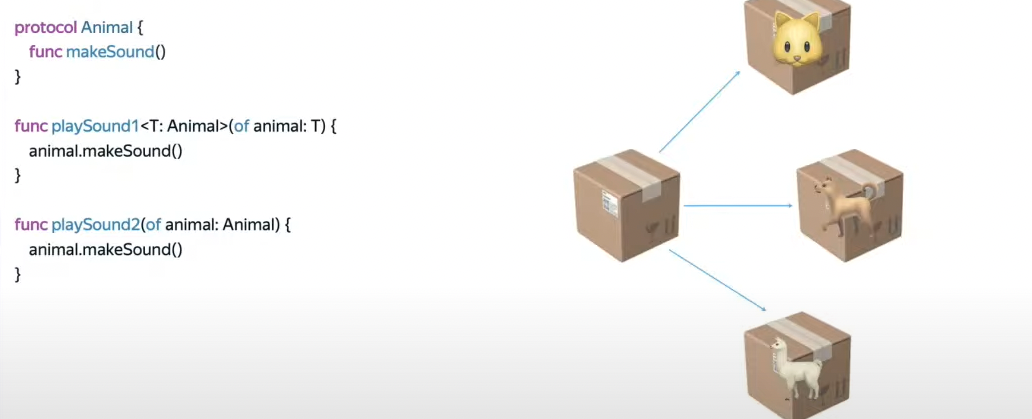
\includegraphics[scale = 0.5]{pic/Снимок экрана 2023-07-28 в 22.53.28.png}
    \newline
    Протоколам могут соотвестсвовать enum классы и структуры, но при этом у них может быть разный размер, а протокол мы хотим использовать в качестве типа. 
    \newline
    Мы не можем как тип аргумента функции поставить что-то неопределенного размера. Existential type -- некоторая коробка, которая имеет фиксированный размер. В этой коробке лежит какой-то объект, который соотвествует необходимому протоколу. 
    \newline
    Это какая-то коробка, в которой что-то лежит, и ни мы, ни компилятор не знаем что. Рассмотрим по внимательнее наши методы, скорее всего не задумываясь мы бы выбрали playSound2, использовав протокол в качестве типа. 
    \newline
    Когда мы используем функции с generic типами, то компилятор может создать на этапе компиляции перегрузки этого метода для всех типов, которые мы можем туда отправить. И когда мы будем вызывать этот метод с определенными параметрами реализация этого метода будет уже готова. Мы будем знать, что мы туда отправили туда, например int, а он уже будет готов. Это статическая диспетчеризация, которая является самой бьыстрой. 
    \newline
    Когда мы используем протокол в качестве типа мы работаем c witness table dispatch, получая накладные расходы. 
    \newline
    Вернемся к протоколам с self, у таких протоколов есть одно важное ограничение, их нельзя использовать в качестве типа. 
    \newline
    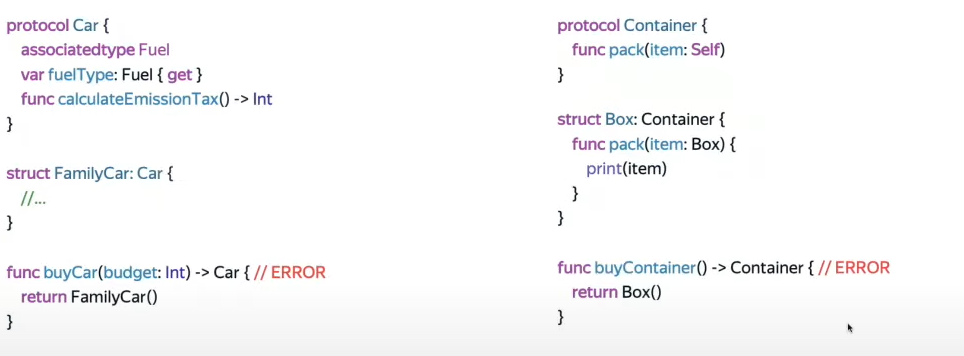
\includegraphics[scale = 0.5]{pic/Снимок экрана 2023-07-28 в 22.59.11.png}
    \newline
    До swift 5.7 мы получали один тип ошибки, а теперь другой тип ошибки, поэтому ERROR.
    \newline
    Вторая ошибка нам напишет, что \swift{any} решит нашу проблему. Оно появилось в swift 5.6 и мы могли применять его к протоколам, но начиная со swift 5.7 мы получили возможность применять его к протоколам с \swift{associated type } и с \swift{self} и использовать их в качестве типа. 
    \newline
    Важно понимать, что когда мы добавляем ключевое слово \swift{any} к протоколу, мы все также работаем с протоколом в качестве типа и работаем с Existensial type.
    \newline
    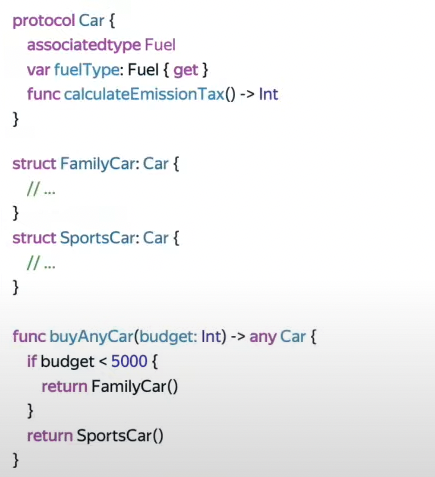
\includegraphics[scale = 0.5]{pic/Снимок экрана 2023-07-28 в 23.02.24.png}
    \newline
    В большинстве случаев нам не нужна такая вариативность, мы не хотим показывать наш тип наружу, а просто хотим закрыть все протоколом такой подход дает вариативность и накладные расходы. Если нам такая вариативность не нужна, мы можем использовать  Opaque type, введя его словом \swift{some}. В данном случае мы возвращаем из buySportsCar opaque type.
    \newline
    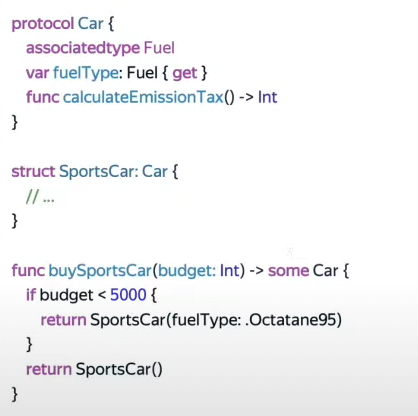
\includegraphics[scale = 0.5]{pic/Снимок экрана 2023-07-28 в 23.05.35.png}
    \newline
    Он в отличии от Existantial type сохраняет идентичность типа. Компилятор имеет доступ к информации о типе с которым мы работаем. Для тех, кто использует этот метод этот тип закрыт протоколом. В данном случае мы и в одном и в другом случае возвращаем sportCar, если мы в одном месте начали возвращать SportCar, а в другом решили вернуть Family это выдаст нам ошибку:
    \newline
    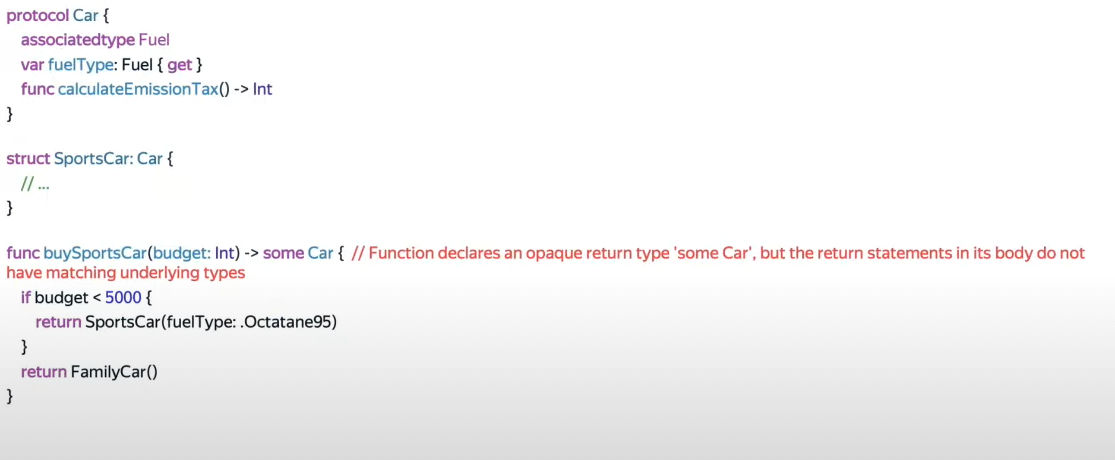
\includegraphics[scale = 0.5 ]{pic/Снимок экрана 2023-07-28 в 23.07.44.png}
    \newline
    Мы работаем с конкпретным типам. Если подумать наглядно, то Opaque type -- какой-то тип, о котором не знаем мы, но знает компилятор, а Existantial type -- вообще непонятная штука, о которой единственное что мы можем сказать, что она соотвествует протоколу. 
    \newline
    Если мы используем протокол в качестве типа, то работаем с Existential type.
    \newline
    В некоторых случаях нам может не хватать информации о Existential type. Рассмотрим пример: 
    \newline
    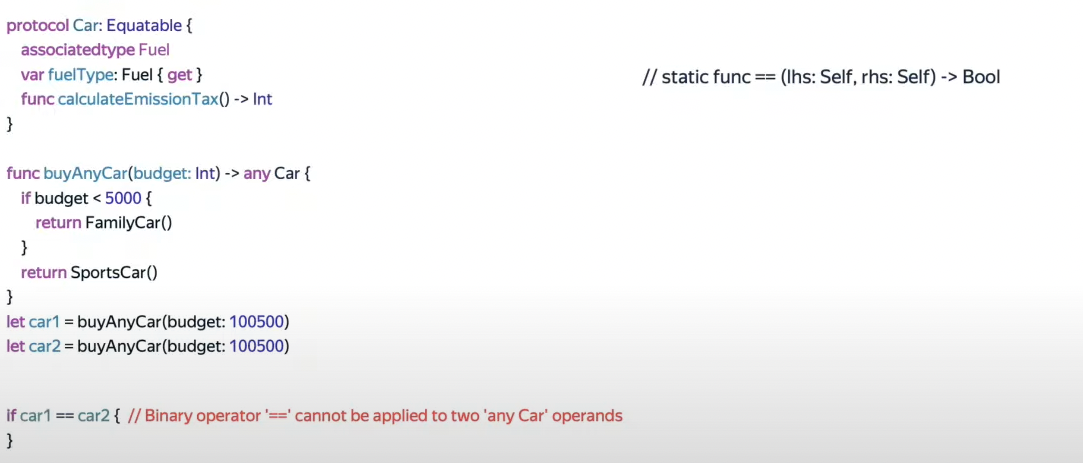
\includegraphics[scale = 0.5]{pic/Снимок экрана 2023-07-28 в 23.14.36.png}
    \newline
    Мы хотим сравнить результат работы этого метода, но при оператора сравнения у нас выскочит ошибка. 
    \newline
    несмотря на то, что проктол car требует, чтобы те, кто ему соотвествовали также соотвествовали протоколу Equatible, мы не можем их сравнить. 
    \newline
    Когда мы хотим что-то сравнивать, мы хотим сравнить и их типы, что они также совпадают. Поскольку мы работаем с Existantial type у нас нет инфмаорации о типе, поэтому оператор сравнения не может проверить, что типы левого и правого аргумента одинаковые и не может их сравнить. 
    \newline
    Если мы работаем с opaque type, то такой проблемы нет, так как компилятор знает с каким типом мы работаем, информация о типе есть и мы можем спокойно сравнить результаты этих методов. 
    \newline
    \newline
    Есть еще одна проблема, рассмотрим протокол: 
    \newline
    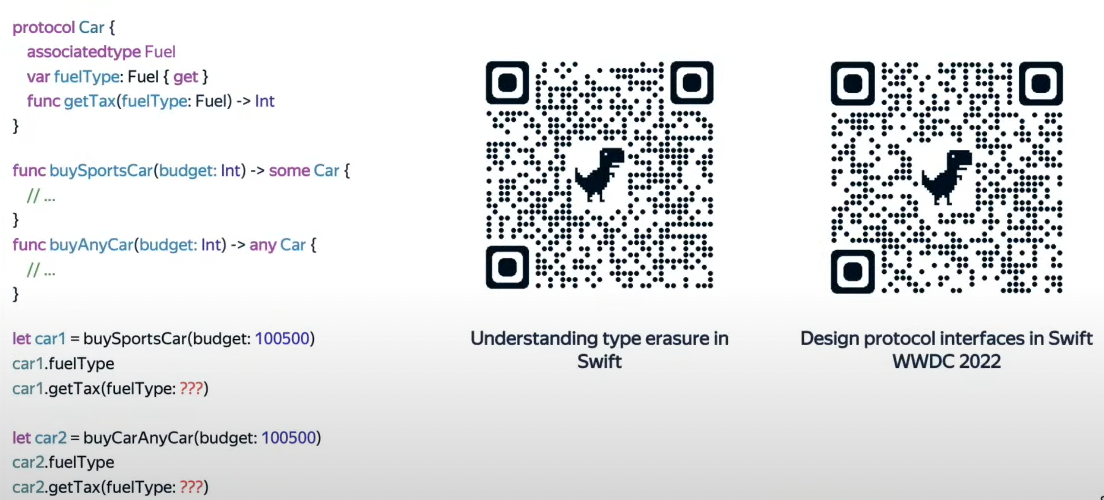
\includegraphics[scale = 0.5]{pic/Снимок экрана 2023-07-28 в 23.19.06.png}
    \newline
    Мы хоим у результатов этих методов выхвать getTax, но при этом мы не знаем какой тип во fuelType, при этом если мы пишем конкретный тип, который мы определили в соответсвии с протоколом, компилятор не даст этого сделать. 
    \newline
    Реншить такую проблему мы можем двумя способами: 
    \newline
    1) Написать свой typeerror -- обертку, которая соотвествует необходимому протоколу и которую мы будем дальше использовать
    \newline
    2) Развернуть asociatedtype и дальше с ним работать. 
    \subsection{Result error}
    Рассмотрим пример: есть какая то стркутура у котрой есть свойство body, которое имеет тип some View.
    \newline
    Кажется, что в зависимости от условия мы вовзращаем либо текст, либо image: 
    \newline
    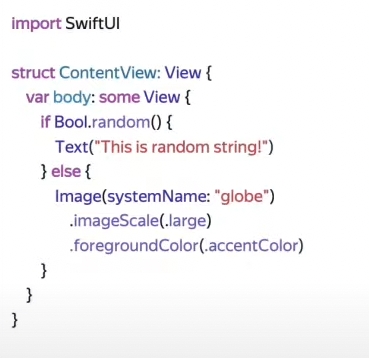
\includegraphics[scale = 0.5]{pic/Снимок экрана 2023-07-28 в 23.47.11.png}
    \newline
    Мы же видели, что так нельзя делать
    \newline
    Рассмотрим как было реализован протокол \swift{View}
    \newline
    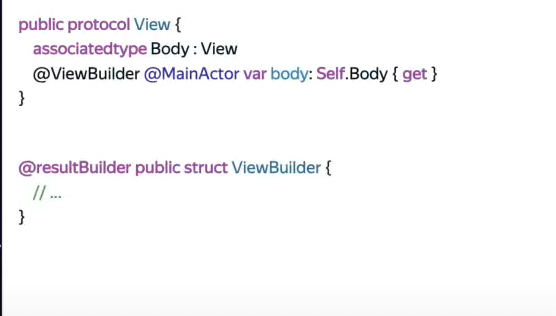
\includegraphics[scale = 0.5]{pic/Снимок экрана 2023-07-28 в 23.48.02.png}
    \newline
    \swift{ViewBuilder} является реализацией \swift{@resultBuilder}. Его можно рассматривать как встроенные domain specific language. Это некоторый предметно ориентированный язык, который описывает объединение частей в окончательный результат. 
    \newline
    \swift{@resultBuilders} позволяют в swift получить результирующие значения из последовательности компонентов, выстроенных друг за длругом так называемых строительных блоков:
    \newline
    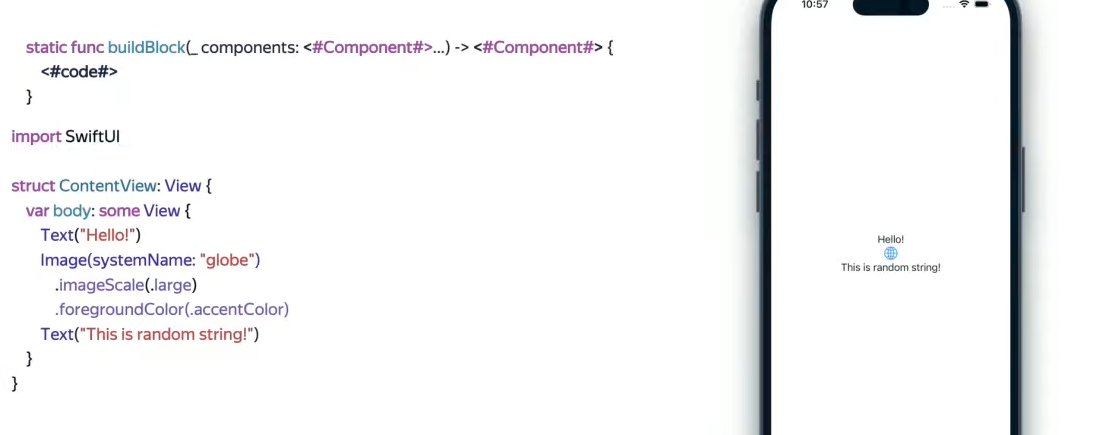
\includegraphics[scale = 0.5]{pic/Снимок экрана 2023-07-28 в 23.50.29.png}
    \newline
    Мы можем реализовать \swift{@resultBuilder} для своих собственных типов. Для этого будет неоходимо обяхательно реализовать только одну фнукцию \swift{BuildBlock} -- принимает переменное количество параметров и при этом возвращает какой-то результат. Важно, чтобы тип аргумента и тип результата совпадал. 
    \newline
    Если его реализовать то получим возможность собирать результат как в функции ContentView -- просто картинка, текст, картинка, текст, без всяких разделителей и каких либо других символов.
    \newline
    \newline
    Вернемся к примеру с if и else:
    \newline
    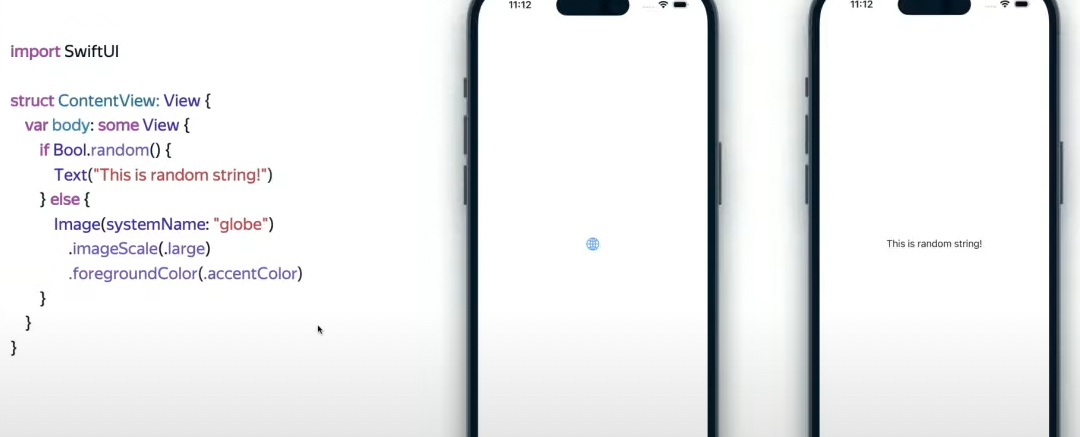
\includegraphics[scale = 0.5]{pic/Снимок экрана 2023-07-28 в 23.55.44.png}
    \newline
    Помимо метода BuildBlock, который просто объединяет накиданные блоки в результат мы также можем реализовать дополнительные методы, которые позволят делать \swift{if} или \swift{if else}. Здесь мы не возвращаем либо text либо image, в зависимости от какого-то условия, это все приводится к одному определенному результату, добавим для наглядности текст к результату: 
    \newline
    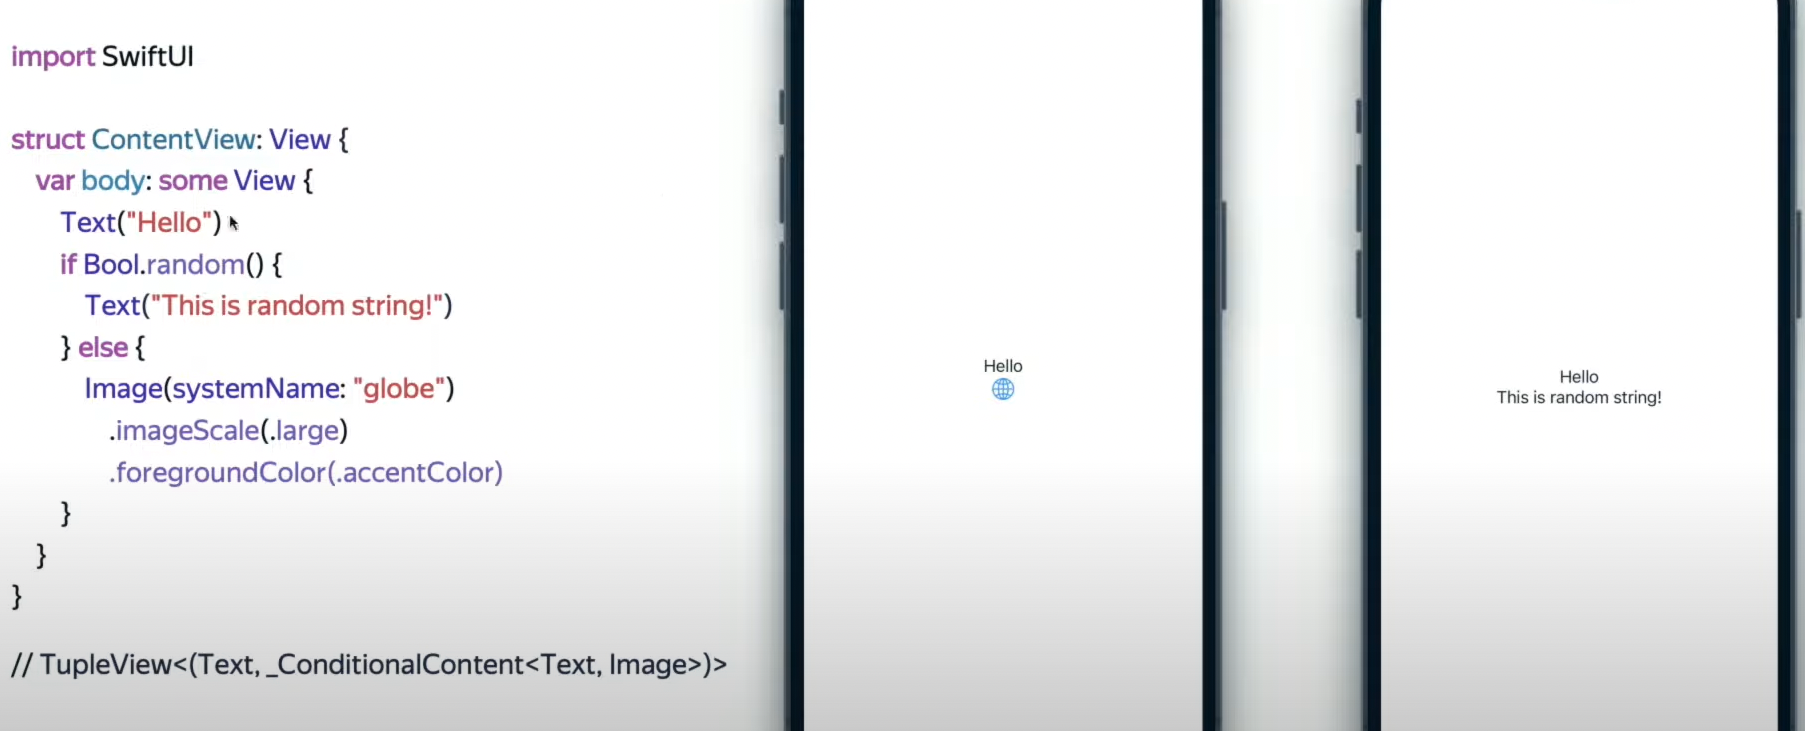
\includegraphics[scale = 0.3]{pic/Снимок экрана 2023-07-29 в 00.00.27.png}
    \newline
    Мы получем определенный результат определенного типа, поэтому мы можем использовать Opaque type и ключевое слово \swift{some}.
    \subsection{Коллекции}
    В swift 3 основных типа коллекций: 
    \begin{enumerate}
        \item Массивы -- упорядоченные коллекции значений
        \item Множества -- неупорядоченные коллекции уникальных значений
        \item Словари -- неупорядоченные коллекции, которые хранят пары ключ значение. 
    \end{enumerate}
    Попробробнее остановимся на множествах и словарях. У нас есть структура set, и иногда нам хочется в нее положить элемент, очень полезная коллекция. 
    \newline
    Но не каждый элемент мы можем полжить в \swift{Set()}, для этого он соотвествовать протоколу \swift{Hashible}. В swift \swift{set()} -- это hashSet
    \subsubsection{Set}
    В set есть скрытый массив, когда мы например хотим положить какую-то строку, в данном случае byte, то от этой строки вычисляется hash функция и мы получаем hash значение -- какой-то целочисленное значение. Мы в этот массив по полученном целочисленному значению кладем наш элемент в ячейку памяти. Бывает, что там уже что-то может лежать, тогда мы должны сравнить, являются ли элементы эквивалентными, потому что если такой элемент уже лежит в множежстве, зачем нам туда его класть. Если такой элемент уже лежит, мы его не кладем, но если они не эквиваленты, мы его кладем с использованием связанного списка, такая ситуация называется коллизией. 
    \newline
    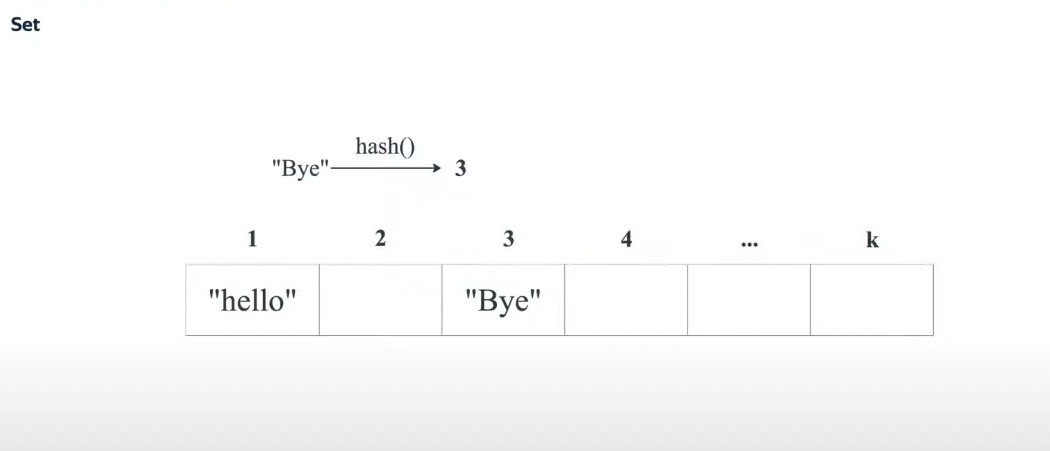
\includegraphics[scale = 0.5]{pic/Снимок экрана 2023-07-29 в 00.15.13.png}
    \newline
    Со словарем происходит такой же принцип, только мы уже вычисляем hashValue от ключа и кладем пару ключ значение. 
    \newline
    Для того, чтобы быть элементом множества, тип этого элемента должен соотвестсвовать протоколу Hashable. Некоторые типы по умолчанию соотвествуют этому протоколу (\swift{String, Int, Double, Set}). Некоторые типы, например \swift{Optional, Array, Range} автоматически становятся Hashable, если их аргументы соотвествуют Hashable. Если мы работаем с Enum у которого нет \swift{associatedValue}, мы также можем с ними работать и они будут являстя hashable без явного указания. Также у нас есть 2 ситуации, когда мы получаем соотвествие этому протоколу бесплатно: 
    \newline
    1) Если мы работаем со структурой и все хранимые свойства структуры соотвествуют протоколу hashable, до достаточно просто дописать в структуру, что она соотвествует протоколу Hashable. Никаких фнукций при этом писать не требуется
    \newline
    2) Если мы рабоатем с Enum, и все \swift{asociatedValue} в enum соотвествуют протоколу \swift{Hashible}, то у этого enum мы тоже бесплатно можем приписать Hashable и использовать его в качестве типа для set или словаря. 
    \newline
    Если верхние условия не выполнены, и типы не удовлетворяют поставленному условию, тогда мы должны самостоятельно, своими руками вызывать 2 метода: 
    \newline
    1) Функция hash, которая должна комбинировать свойства, которые мы туда добавим и вычислять hashValue с помощью hasher
    \newline
    2) Функция сравнение, она может быть полезна, когда мы что-то хотим положить в set() и сравнить. 
    \newline
    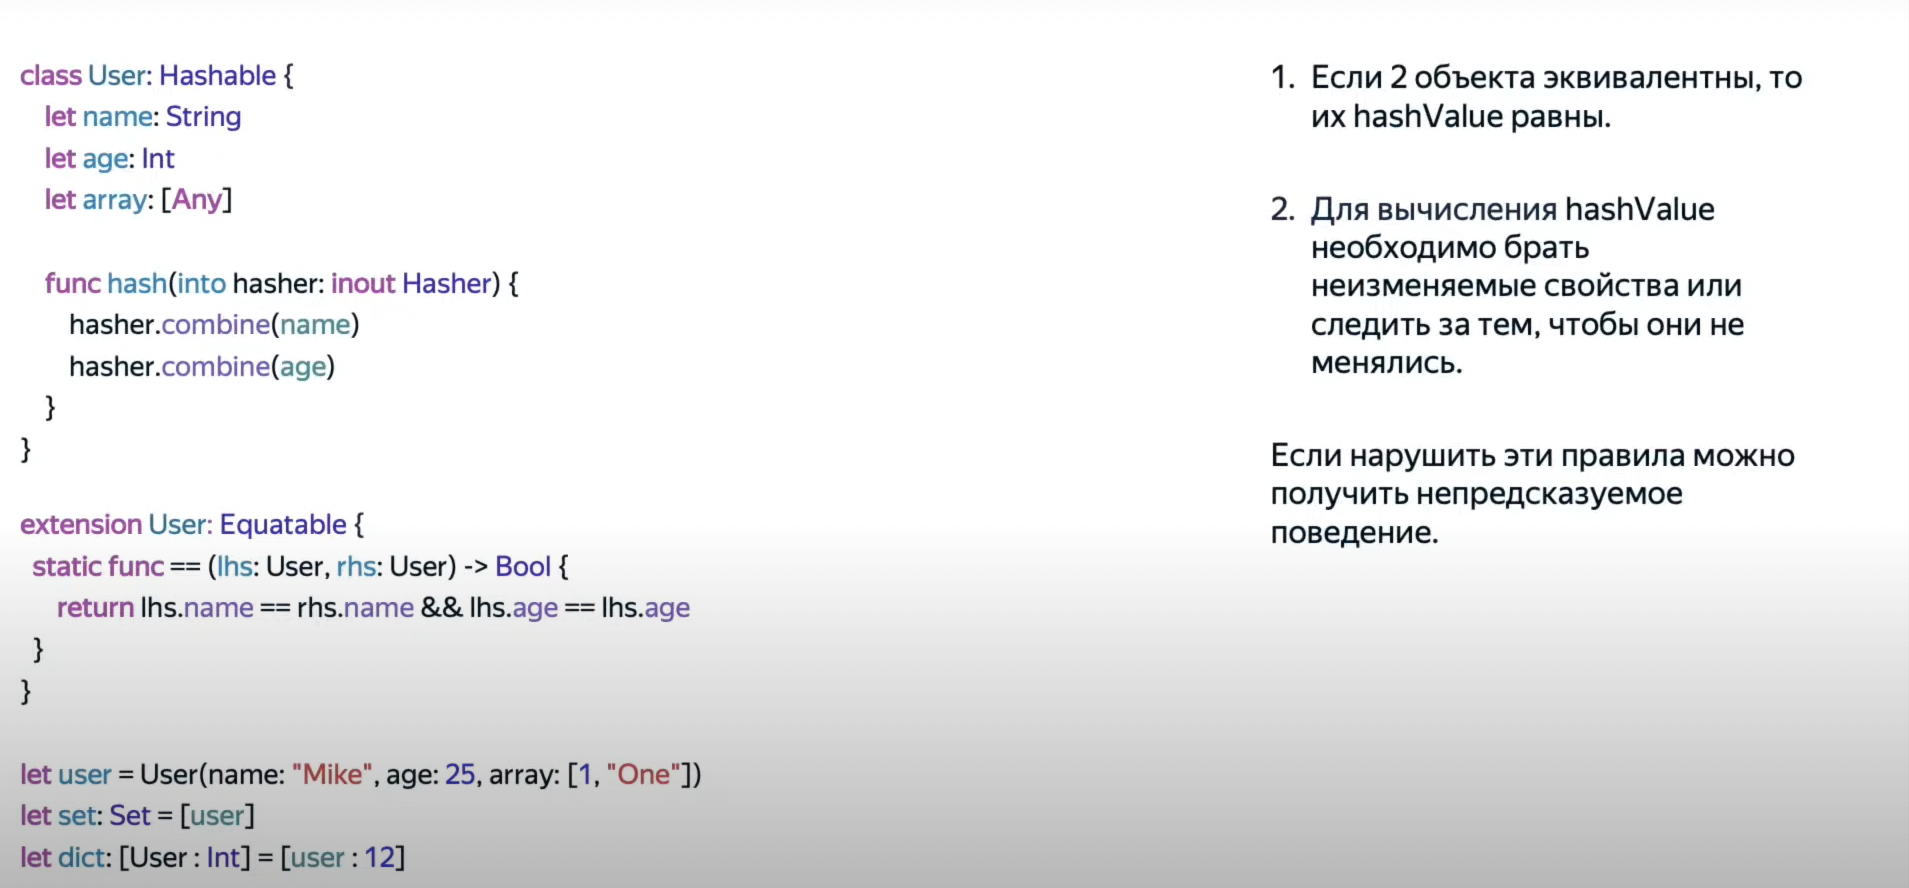
\includegraphics[scale = 0.2]{pic/Снимок экрана 2023-07-29 в 00.24.10.png}
    \newline
    Очень важно соблюдать 2 правила: 
    \newline
    1) Если 2 объекта равны, то и их hashValue() должны быть равны. Этого можно достичь, используя одни и те же свойства при проверки эквивалентности и в функции hash
    \newline
    2) Для hashValue лучше брать неизменяемые свойства или следить, чтобы они не менялись. 
    \newline
    Если мы нарушим эти свойства, то мы можем получить неопределенное поведение. 
    \newline
    Swift частично поддерживает падигмы функционального программирования, например, мы можем использовать функции васшего порядка, которые принимают функции как аргумент. Это очень удобно при работе с коллекциями, рассмотрим самые популярные из них: 
    \newline
    \includegraphics[scale = 0.5]{pic/Снимок экрана 2023-07-29 в 00.32.22.png}
    \newline
    \textbf{map} -- применяет метод к каждому аргументу коллекции. Принимает на вход функцию, которая принимает один параметр. В данном случае \$0 мы заменяем на первый аргумент функции  
    \newline
    \textbf{compactMap} -- map, но если появляются nil значения, они удаляются из результата. 
    \newline
    \textbf{faltMap} -- убирает одну вложенность, а так работает как map.
    \newline
    \textbf{filter} -- применяет условие к каждому элементу коллекции и возвращает колекцию, которая соотвесвует этому условию. 
    \newline
    У нас есть 3 основные типа коллекций, обычно нам достаточно их для рабочих задач. Но допустим нам недостаточно тех типов коллекцйи, тогда мы можем создать свою коллекцию. Для того, чтобы это делать познакомимся с основными протоколами, которые лежат в основе всех коллкций: 
    \newline
    \includegraphics[scale = 0.5]{pic/Снимок экрана 2023-07-29 в 00.36.28.png}
    \newline
    Напишем структуру, которая ляжет в основу нашей коллекции:
    \newline
    \includegraphics[scale = 0.5]{pic/Снимок экрана 2023-07-29 в 00.38.42.png}
    \newline
    Теперь посмотрим, как легко мы можем соотвестсвовать протоколу \swift{Collection}:
    \newline
    \includegraphics[scale = 0.3]{pic/Снимок экрана 2023-07-29 в 00.39.52.png}
    \newline
    \includegraphics[scale = 0.3]{pic/Снимок экрана 2023-07-29 в 00.43.00.png}
    \section{Архитектура iOS}
    \subsection{Что есть хорошая архитектура, а что такое плохая архитектура}
    Архитекутра -- своего рода фундамент, на основе которого мы строим наше приложение. \textbf{Архитектура программного обеспечения} -- совокупность \textbf{важнеших решений} об организации программной системы. 
    \newline
    Таким образом архитектура -- то, на чем все строится, архитекутрные решения поменять очень сложно. Как правило это выражается в больших временных затратах, либо в денежных затратах. 
    \newline
    При этом архитекутра -- то с чем мы сверяем свои решения при разработке конкретных модулей нашего приложения. 
    \newline
    Как же понять, хорошая ли наша архитектура или нет, выведем некоторые принципы: 
    \begin{enumerate}
        \item \textbf{Архитектура --} это инструмент, который мы всегда используем. Первый признак того, что все хорошо -- то, что мы это используем. 
        \item  Минимальная дискуссионность, при разработке компонентов системы мы скорее дискутируем о том, как конкретные выбранные решения ложаться на архитекутрные принципы, нежели о самих принципах. Новые фичи хорошо ложаться на архитекутру, при этом не возникает проблем с их реализации. Если при этом возникают новые вводные по поводу самой архитектуры, их легко можно в нее уложить в выбранные принципы. 
        \newline
        Они работают вместе, очень странно, когда часть нашего приложения написана в одних архитекутрных принципах, а другая в других. и мы начинаем изобретать костыли между двумя разными подходами. 
        \item  Любая сущность в нашем коде нужна для чего-то и это понятно не только тому, кто писал этот код, но и тем, кто его читал, кто пытается разобраться в том, как этот код работает. Если вдруг возникает необходимость UnitTest у нас не возникает трудностей с этим. Если возникают сложные связи -- скорее всего что-то там не так. 
        \newline
        
    \end{enumerate}
    \subsection{Базовые паттерны}
    \textbf{Паттерн } -- некоторая идея, про то, как рещать конкретную задачу. Это устойчивое решение определенной технической проблемы. 
    \newline
    Как оформлять какой-то программный код, решающий конкретную задачу, мы рассмотрим 3 из них: \textbf{delegate, observer(наблюдатель) и responder chain(цепочка отвественных)}. 
    \subsubsection{delegate}
    \textbf{Делегированние} -- передача части своих обязанности другим сущностям. Рассмотрим как будет выглядеть бариста в программном коде: 
    \newline
    \includegraphics[scale = 0.5]{pic/Снимок экрана 2023-07-29 в 14.54.36.png}
    \newline
    Обычно для того, чтобы сущность, которая что-то делигирует не знала конкретный класс и тому, кого она делигирует заводится протокол. В этом протоколе объявляется то, что мы хотим третий сущности делигировать. В данном примере мы хотим делигировать право выбора напитка, температуры и хотим делигировать некоторые другие действия. В класе Barista мы объявляем delegate , обычно объявляются слабой ссылкой, чтобы не реализовывать циклические зависимости. Когда бариста готовит кофе он вызывает поля или методы delegate, чтобы делигировать delegate о процессе приготовления кофе. 
    \subsubsection{Наблюдатель}
    \textbf{Наблюдатель --} поллучение уведомления об изменении состояния внешнего объекта. Рассмотрим метафору на подписки на газеты: 
    \newline
    \includegraphics[scale = 0.5]{pic/Снимок экрана 2023-07-29 в 14.59.10.png}
    \newline
    Важно здесь то, что наблюдатель для начала выражает заинтересованность в получении каких-то обновлений, какой-то информации. И затем publisher, когда случается что-то, например, выходит новый экземпляр газеты. Он всем, кто изъявил получать уведомления говорит о том, что новый экземпляр вышел. Если мы будем говорить о коде, то это может выглядеть следующим образом: 
    \newline
    \includegraphics[scale = 0.5]{pic/Снимок экрана 2023-07-29 в 15.00.49.png}
    \newline
    Считается хорошей практикой, что наблюдатель может отказаться от подписки. 
    \newline
    Если мы будем говорить об iOS SDK, там есть несколько часто употребимых наблюдателей: 
    \begin{itemize}
        \item KVO -- Key-Value Observing , когда мы можем подписаться на изменение какой-то сущености и следовательно получасть изменения, когда это поле изменяется. Даже привычные will set, не совсем KVO, но похожая история. 
        \item Notification Center -- позволяет получать push или какие-то локальные уведомления. 
        \item Combine: Publisher/Subscriber -- выделенные сущности с большим букетом функций. 
    \end{itemize}
    \subsubsection{Цепочка отвественных}
    Заключается в том, что когда нам нужно решить какую-то задачу, у нас есть некоторая цепочка, выстроенная по какому-то принципу, например, по принципе размещения. Используется для определения conrola который будет отвечать за татти отвечать. 
    \newline
    Выглядит это так: есть некоторая цепочка, выстроенная из связей. Приходит вопрос, кто дежурный например. Участники команды знают, у кого спросить. Таким образом они могут проверить, кто дежурный. Как это выглядит в коде? 
    \newline
    \includegraphics[scale = 0.5]{pic/Снимок экрана 2023-07-29 в 15.07.59.png}
    \newline
    Есть некая сущность, которая может сказать, что она дежурный, либо знает кому делигировать этот выбор. Мы можем построить эту цепочку и настроить делигирование. Внешняя сущность с помощью этой цепочки может этот вопрос решить. 
    \newline
    В iOS SDK самый яркий пример цепочки отвественных -- responder chain для выбора того, кто будет touchи будет обрабатывать. 
    \subsection{Компонент}
    На базе абстракций компонента мы можем рассмотреть обе основные архитектуры. Она поможет декомпозировать конкретные архитектуры и сказать, насколько хорошо выглядит один компонент какой-то конкретной архитектуры. 
    \newline
    \textbf{Компонент} -- сущность, выраженная в классе или структуре. Она необходима нам для решения одной какой-то конкретной задачи. 
    \newline
    \includegraphics[scale = 0.5]{pic/Снимок экрана 2023-07-30 в 18.27.25.png}
    \newline
    У компонента есть входные данные(данные, которые нужны компоненту для решения этой задачи) и выходные данные(данные, которые получаются в ходе решения этой задачи)
    \newline
    Также компоненту нужны еще 2 вещи: зависимости(внешние ресурсы без которых компонент не сможет решить свою задачу) и также конфигурация(в зависимости от конфигурации компонент может решать свою задачу по разному)
    \newline
    Если говорить о \swift{Barista}, рассмотрим его как компоненту: 
    \newline
    \includegraphics[scale = 0.5]{pic/Снимок экрана 2023-07-30 в 18.30.15.png}
    \newline
    У баристы есть 2 пути передачи входных данных(in \#1 и in \#2). Первые -- входные данные, которые передаются экземпляру этого класса в целом, например сегодня это меню. Собственно этот набор вожных данных существует всю жизнь лица баристы. 
    \newline
    Второй набор входных данных -- входные данные одного наполнения баристы. У каждого такого процесса выполнения задачи может быть свой набор входных данных.  Входные данные второго типа используются не все время жизни баристы, а только во время одного конкретного запроса(действия). Соотвественно выходные данные также могут существовать в двух вариантах: 
    \newline
    1) Результат всей жизнедеятельности баристы. С точки зрения баристы -- деньги заработанные за день
    \newline
    2) Как результат одного действия -- чашка кофе.
    \newline
    И зависимость и некоторую конфигурацию мы можем передать либо в инициализаторе сущности, например молоко зерна и тд.Соотвественно можно выдать конфигурацию: например, не готовить капучино с 12-ти часов. 
    \subsection{Apple MVC} 
    Первая, классическая архитектура, ей много лет. Активно применялась до возникновения iOS. 
    \newline
    \swift{Apple MVC} -- вариант архитектуры Model View Conroller, в котором явным образом выделяются 3 явных сущности: Модель, представление и контроллер: 
    \newline
    \includegraphics[scale = 0.5]{pic/Снимок экрана 2023-07-30 в 18.38.12.png}
    \newline
    Стоит отметить одну вещь, которая справедлива и для MVC и для MVI: квадратик на этой и остальных схемах не означает что это класс, обычно модель -- набор классов, которые друг с другом связаны. У больших приложений модели могут содержать большое количество классов и это не значит, что это все одна сущность. 
    \newline
    Модель это какая-то бизнесн-логика, в которой обрабатывается сущность нашего приложения. 
    \newline
    Представление -- то, что пользователь видит и через что взаимодействует. 
    \newline
    Контроллер -- то, что связывает 2 сущности воедино.
    \newline
    Рассмотрим каждый из элементов согласно концепции компонента. 
    \subsubsection{View}
    Если мы посмотрим на View, то увидим, что входные данные у него одни и представление нужно для того, чтобы эти данные пользователю отражать. 
    \newline
    А если мы посмотрим на выходные данные, то их 2 штуки: 
    \newline
    1) Пиксели на экране, которые видит пользователь и через которые воспринимает эту информацию. 
    \newline
    2) Действие, которые пользователь оказывает, через это представление. 
    \newline
    В некоторых реализациях MVX представление нужно именно для того, чтобы данные отобразить пользователю, а воздействие осуществляется через другой механизм. 
    \newline
    Первый тип выходных данных нам не очень интересен. Мы будем рассматривать View только как что-то через что мы можем получить пользовательские данные:
    \newline
    \includegraphics[scale = 0.2]{pic/Снимок экрана 2023-07-30 в 18.49.59.png}
    \newline
    Это псевдокод, как может выглядить эта компонента. Метод setup() -- передача данных для отображения пользователю. Дальше у нас есть некоторая кнопка, с которой пользователь взаимодействует: выходные данные нашей View
    \subsubsection{Модель}
    Похожа на классический компонент. Получает на вход некоторые данные о пользовательских действиях, на базе них происходит внутренний общет и на выходе у нас есть уведомление о том, что модель изменилась. Примерно так и в коде: 
    \newline
    \includegraphics[scale = 0.3]{pic/Снимок экрана 2023-07-30 в 18.52.36.png}
    \newline
    Модель здесь выглядит как классический компонент. Мы можем передать пользовательское воздействие через метод update(), что-то внутри модели изменится и собственно говоря, когда title изменится сообщим о том, что модель изменилась(в данном случае через делегатный метод)
    \subsubsection{Контроллер}
    Центральный компонент. Увидим, что у нас есть 2 набора входных и выходных данных: 
    \newline
    \includegraphics[scale = 0.5]{pic/Снимок экрана 2023-07-30 в 18.54.16.png}
    \newline
    Здесь явным образом нарушается принцип линейной ответсвенности, контроллер не является компонентом в чистой виде, а является суперпозицией двух компонент. Это в некотором роде приводит к проблеме известной как messyViewController, когда во ViewController складывается больше, чем в нем по идее должно быть. 
    \newline
    \includegraphics[scale = 0.5]{pic/Снимок экрана 2023-07-30 в 18.56.10.png}
    \newline
    Через механизм подписки, например, получает увдомление о измении пользовательских действий и передает их в соседнюю компоненту. 
    \newline
    Таким образом, рассматривая архитектуру MVC с точки зрения наших принципов можно сказать следующее: компоненты разделены, однако никто особо не говорит, как строить бизнес-логику. Толкования порождают разные варианты решения этой проблемы и некоторые приводят к messyViewController
    \newline
    Мы можем написать unitTest, так как все части похожи на компоненты, но с контроллерами будут проблемы.
    \newline
    В целом архитектура доступна для понимания, легко начать, легко использовать, легко придти к проблемам. 
    \newline
    Стоит упомянуть о всем классе MVx архитектур: 
    \newline
    \includegraphics[scale = 0.5]{pic/Снимок экрана 2023-07-30 в 18.59.53.png}
    \newline
    В целом как бы мы MVx архитектуру не назвали она остается примерно той же самой. Разве что меняется название контроллера. Вне зависимости от того, как мы назовем его остается неотвеченными следщующими вопросы: 
    \begin{enumerate}
        \item Как устроен backend приложений, хождение в сеть и тд. В некотором роде VIPER, в котором больше функциональных компонентов пытается ответить вопрос, но обычно это не рассматривается
        \item  Есть вопросы навигации и такие вещи например, как обработка диплингов. Вынуждены делать как получиться. 
    \end{enumerate}
    
    \subsubsection{Чем принциально отличается модель от представление}
    Ничем, кроме актора, который вполняет действия. Если мы говорим про представление, то этим актором является польователь. В случае модели этим актором является код, который мы написали. В остальном и модель и представление входные данные оперделенным образом преобразует в выходные.
    \subsection{Model-View-Intent(MVI)}
    Эту архитектуру мы можем найти под разными названиями. \textbf{MVI} -- наиболее употребимое. Также такие подходы мы можем встретить в \textbf{UDDF(Unit Directory Data Flow)}.
    \newline
    В чем заключается идея этой архитектуры? 
    \newline
    \includegraphics[scale = 0.5]{pic/Снимок экрана 2023-07-30 в 21.39.55.png}
    \newline
    В этой архитектуре есть несколько больших компонентов, самый важные -- компонент состояние(на картинке -- глобальное состояние S) и соотвественно некая сущность, везде называется по разному(где-то reducer, где-то extion executor) щтука, которая изменяет состояние. Есть классическое представление, которое отображает это состояние пользователю и обрабатывает пользовательский ввод и какой-то набор сервисов, которые внутри себя инкапсулируют бизнес-логику. 
    \subsubsection{Состояние}
    Состояние -- это состояние, единственный источник истины о состоянии нашего приложения в данный конкретный момент времени, хранится слепок всего состояния нашего приложения. 
    \newline
    \includegraphics[scale = 0.5]{pic/Снимок экрана 2023-07-30 в 21.44.29.png}
    \newline
    С точки зрения компоненты входные данные -- входные данные -- поток изменения состояния от reducer. Выходные данные -- слепок текущего состояния для любого потребителя. 
    \newline
    Состояние является классическим компонентом. В коде можно выразить так: 
    \newline
    \includegraphics[scale = 0.5]{pic/Снимок экрана 2023-07-30 в 21.46.06.png}
    \newline
    Есть набор данных(текущее состояние) и способ подписаться на его изменение(методом, keyValueOBserving, Combine(Publisher)), каким угодно способом мы можем подписаться не только на текущее состояние, но и на его получение. 
    \subsubsection{Представление}
    Представление почти не отличается от подхода в MVC: 
    \newline
    \includegraphics[scale = 0.5]{pic/Снимок экрана 2023-07-30 в 21.47.49.png}
    \newline
    В целом представление здесь по прежнему представляет классическую компоненту:
    \newline
    \includegraphics[scale = 0.2]{pic/Снимок экрана 2023-07-30 в 21.48.52.png}
    \newline
    Эта архитектура подходит скорее для SwiftUI, но ее также можно использовать в приложении с UIKit, на самом деле разнгица только во фреймворке который мы используем и как передаем данные. В целом эту архитектуру можно использовать и в нашем текущем приложении, если мы хотим мигрировать на SwiftUI.
    \newline
    Setup настраивает представление. Если кто-то кнопку нажал здесь уже есть разница, мы не напрямую воздействуем, а через closure или протокол actionExecutor мы выдаем действие в систему. Архитектура называется ModuleViewIntend, и Intend -- намерение действие пользователя выражается в виде сущности, которая иногда называется intend, иногда называется action. Мы здесь в представлении выдаем какое-то действие в систему. 
    \newline
    Если мы внимательно посмотрим на схему, между представлением и reducer есть желтый квадратик -- reducer. Собственно говоря View должна по хорошему поменьше знать об action, она должна оперировать в своих собственных понятиях, и в ее понятиях должна выдавать в систему, что кнопка нажата. Не о каком-то конкретном действии, а о том, что кнопка нажата. А адаптер(reducer) из понятия о том, что кнопка нажата преобразует его в конкретный action, что надо поменять title. Когда мы будем писать код лучше эти действия разделять. 
    \newline
    Если мы говорим про swiftUI, то все будет примерно также: 
    \newline
    \includegraphics[scale = 0.3]{pic/Снимок экрана 2023-07-30 в 22.03.34.png}
    \newline
    Единственно, нам надо предосматреть такую сущность как observableObject, чтобы магия swiftUI работала. Его также можно звать \swift{viewModel}, частое название. View его использует. Когда кто-то меняет titile происходит дерево отображения SwiftUI. Выходные действия делаются также, как в UIKit, есть actionExecutor. Но лучше все равно делать с использованием adapter преобразовать его в changeTitleAction.
    \subsubsection{Сервис(Service)}
    В архитектуре MVC мы называли это моделью. Это компонент, который релизует конкретный набор бизнес-логики. Соответсвенно входными данными для сервиса является изменения state. Заметим одну вещь, в MVC это было пользовательскими воздействиями на представление. Здесь важно, что это всегда изменение state, в том числе это может быть порождено другим сервисом, необязательно пользовательским воздействием на представление. У нас и бекграунд сервисы, и представления в некотором роде друг от друга развязаны, им не надо друг о друге знать. 
    \newline
    \includegraphics[scale = 0.5]{pic/Снимок экрана 2023-07-30 в 22.09.02.png}
    \newline
    \includegraphics[scale = 0.3]{pic/Снимок экрана 2023-07-30 в 22.09.39.png}
    \newline
    В коде это может выглядеть так. Пришло изменение состояние в функцию notify и мы генерируем новое изменение состояние. Если рассматривать composableArchitecure там есть эффект. И смотря на этот код можно скзаать, что это одно и то же. В конктексте терминов dependencyEjection эффект является прототипной сущностью. На каждый новый эффект генерируется новый. А Серивс является персистентной сущностью, которая существует всегда и просто обрабатывает новые изменения. Через серивис такие вещи реализовать проще, потому что эффектом может быть запрос бекенд. И когда у нас это в сервисе, сервис может держать токен текущего запроса, ну если пришел еще один такой-же еффект -- отменить старый и спросить новый. Если мы работаем в рамках эффекта и прототипа сущностей, нам нужно еще какую-то сущность изобрести, которая будет держать этот токен. И это сложно и порождает лишнего кода, который в такой абстракции было бы написать гораздо проще
    \subsubsection{Observer}
    Маленькая компонента, наблюдатель состояния. Он обеспечивает не только поставку слепка текущего состояния всем заинтересованным сущностям, но и сигнал оьб его изменении, который позволяет реализовать реактивный подход к анализу изменения состояний. 
    \newline
    \includegraphics[scale = 0.5]{pic/Снимок экрана 2023-07-30 в 22.15.22.png}
    \newline
    На выходе дает примитив, на который можно подписаться, как на реактивный поток изменений состояния. В коде выглядит так: 
    \newline
    \includegraphics[scale = 0.5]{pic/Снимок экрана 2023-07-30 в 22.16.29.png}
    \newline
    В данном случае реализует наблюдатель состояний. 
    \subsubsection{Исполнитель действий}
    С другой стороны, reducer или action executor это штука, которая принимает поток действий по изменению состояния. А действия -- иммутабельная сущность которая хранит в себе информацию о том, как состояние изменить. Можно рассматривать действие как письмо куда-нибудь с каким-то указанием. Соотвественно оно на вход принимает действия, а на выход дает новое состояние. 
    \includegraphics[scale = 0.5]{pic/Снимок экрана 2023-07-30 в 22.18.39.png}
    \newline
    Сущность reducer выполняет сущность reduce, из двух операндов получает новое состояние. 
    \newline
    В коде это может выглдеть вот так: 
    \newline
    \includegraphics[scale = 0.5]{pic/Снимок экрана 2023-07-30 в 22.19.35.png}
    \newline
    В самом простом случае это просто некоторая функция execute(). В зависимости от того, чем является action изменяет состояние, попутно тригеря наблюдателя состояний. 
    \newline
    Есть еще квадратик -- \textbf{Адаптер}. Он связывает 2 сущности, например -- представление и состояние или состояние и сервис. Просто желательно, чтобы компоненты знали друг по друга по меньше. Это и обеспечивает адаптер. Слабая связанность такой архитектуры -- хорошо. Позволяет переиспользовать сущности, тестировать их.
    \subsubsection{Резюмируя}
    \includegraphics[scale = 0.5]{pic/Снимок экрана 2023-07-30 в 22.22.22.png}
    Работа с такой архитектурой сложна для понимания, в ней больше сущностей, и работает она немножко не так, как все привыкли. В любом случае мир не стоит на месте. Это хорошая архитектура для SwiftUI.
    \subsection{Dependency injection}
    Очень важная штука при разработке приложений. \textbf{Dependency Injection} -- процесс предоставления внешней зависимости программному компоненту. Но чтобы лучше понять рассмотрим пример: 
    \newline
        \includegraphics[scale = 0.5]{pic/Снимок экрана 2023-07-31 в 00.52.26.png}
    \newline
    BookManager хочет работать с книжками, ему нужен серив для работы с книжками. Этот пример без внедреняя зависимостей, то есть \swift{BookManager} прямо сам знает конкретный класс сервиса работы с книжками, он сам его дистанцирует и сам управляет его временем жизни. В некотором роде это плохо, мы не можем заменить сервис, мы не можем варировать его в зависимости от конфигурации, мы не можем в тесте подсунуть что-то туда, чтобы затестить BookManager. Вообщем плохо. Задача внедреняя зависимостей -- передать какую-то реализацию для сервиса, при этом он, как правило про конкретные классы знать не должен. Тогда у нас свобода маневров для изменения этого класса в runtime в зависимости от конфигурации, или в тестах. Как мы можем это сделать? 
    \newline
    В контексте внедреняя зависимостей, зависимости делятся на 2 больших класса: 
    \begin{enumerate}
        \item Синглтон (не паттерн) не смотря на одинаковое название, имеет другой смысл. Паттерн синглтон -- класс или какая-то сущность, которая может иметь ровно один экземпляр. В контексте внедреняя зависимостей, заивисимость типа синглтон существует в одном экземпляре. Мы можем иметь несколько instance этого класса, но в рамках контейнера, в котором мы осуществляем внедренее зависимостей это всегда будет одна и та же сущность.  
        \item  Прототип -- прямая противоположность. На каждый новый запрос instance этой сущности будет генерироваться новый экземпляр. Чашка кофе, которую наливает бариста в нашем примере выше -- прототип. Он каждый раз наливает совершенно новую чашку. 
    \end{enumerate}
    Внедрять зависимости мы можем 3-мя способами: 
    \begin{enumerate}
        \item Через инициализатор, или через то, что является конструктором этого объекта (initializer injection). 
        \item Через свосйтво, или метод установки свройства (property injection)
        \item через интерфейс (interface injection)
        \item Инъекция через окружение (enviroment inhjection)
    \end{enumerate}
    Потому, как выглядит агент, который внедряет зависимость есть 3 возможных подхода: 
        \begin{enumerate}
        \item Фабрика, обычно генерит prototype зависимости. В ней вся суть. И контейнер, и service локатор могут являться фабриками для генерации prototype зависимостей. 
        \item  Контейнер, часто упоминаемый как iOc контейнер, это сущность, которая управляет временем жизни сущностей и настраивает связи между ними. Важно, что про нее никто не знает. 
        \item Servive locator -- то, откуда можно запросить зависимость из любой части кода. 
    \end{enumerate}
    Посмотрим как выглядят конкретные подходы каждого из вариантов: 
    \subsubsection{Инициализатор}
    Все просто, вместо создания зависимости непосредственно в коде, просто передадим ее через инициализатор: 
    \newline
    \includegraphics[scale = 0.5]{pic/Снимок экрана 2023-07-31 в 01.06.33.png}
    \newline
     Почему это хорошо? Мы явным образом требуем зависимости на уровне компиляции, иначе мы не сможем сообрать код. Проверяется компилятором, пользователь видит зависимости, нужные для работы этой сущности. Большую часть времени рекомендуется пользоваться именно этим способом
    \newline
    Но есть и минусы, нужно иметь все зависимости на момент создания объекта. Есть также проблемы с ленивым создания зависимостей, их можно сделать, но конструкции становятся достаточно сложными, нужно делать через pattern провайдера. Также нельзя на первый взгляд создать циклическую зависимость. Но есть трюк через force unwrapping, это тот самый случай  когда это необходимо.
    \subsubsection{инъекция через свойство}
    Тут совсем все просто, мы объявляем свойство и в него просто проставляем нужную зависимость: 
    \newline
    \includegraphics[scale = 0.5]{pic/Снимок экрана 2023-07-31 в 01.11.34.png}
    \newline
    Во первых мы не обязаны иметь все зависимости созданными на момент инициализации view. Делать ее просто -- создали оба объекта и все хорошо. Однако, несмотря на кажущуюся простоту есть проблемы: 
    \begin{enumerate}
        \item Создаем проблемы в продакшне. Если мы вдруг забудем проставить эту зависимость, то особенно при использовании force unwrapping можем получить краш, с которым мы ничего уже не сделаем. Компилятор нам не подскажет об этом, в отличии от инъекции с инициализацтором. 
        \item Пользователь нашей сущности не понимает весь набор зависимостей, которой нашей сущности нужен для работы. Он может просто забыть ее передать и даже не заметить это сразу. 
    \end{enumerate}
    Несмотря на то, что в некотрых случаях она нужна, и ей надо пользоваться она опасна и при прочих равных предпочитать инъекцию с инициализатором. 
    \subsubsection{Инъекция через интерфейс}
    Может быть и через инициализатор и через свойство. Суть в том, что вместо поставки конкретного класса мы используем интерфейс(протокол), тем самым получаем возможность передать туда любую реализацию контракта двух сервисов: 
    \newline
    \includegraphics[scale = 0.5]{pic/Снимок экрана 2023-07-31 в 01.16.18.png}
    \newline
    Можно подставить разные реализации(LSP, Fake в тестах.), большой простор для подстановки реализаций. Каких-то вопросов против не имеет. Всегда стараемся использовать интерфейс/протокол вместо конкретного класса. 
    \subsubsection{Инъекция через окружение}
    Инъекция через окружение -- инъекция через дополнительную сущность, которая называется либо окружением либо контекстом. Мы где-то складываем вещи с сущностью, передаем их целиком, и в нужном месте из нее достаем:
    \newline
    \includegraphics[scale = 0.5]{pic/Снимок экрана 2023-07-31 в 01.19.06.png}
    \newline
    Если мы посмотрим на SwiftUI и про большую иерархию вложенных сущностей мы поймем, что нам достаточно часто нужно через промежуточные сущности передать большой набор элементов, которые им не нужны, но они нужны где-то глубже, поэтому их нужно передать. Это можно реализовать через механизм окружения. Нужно правда его релизовать(но в SwiftUI уже реализован). Так как нам нужно сделать слабую типизацию не всегда удается сделать безопасные способы передачи зависимости. Кое-где нужен downcast, что обычно является источником ошибок. 
    \newline
    Инъекция через окружение имеет область применимости, но следует ее использовать вдумчиво
    \subsubsection{Фабрика}
    Обычно служит для создания завимистей, сущность с набором методов или одним методом, которая генерит эти зависимости. Фабрика может являться окружением. В ней можно хранить зависимости, которые мы подсовываем в генерируемые сущности:
    \newline
    \includegraphics[scale = 0.3]{pic/Снимок экрана 2023-07-31 в 01.27.13.png}
    \newline
    Таким образом \swift{makeBookService()} может не содержать аргументов, а все нужные зависимости для \swift{BookServiceInpl} хранится в своей фабрике. Позволяет спрятать инжективную зависимость. 
    \newline
    Можно неявно пробросить зависимости. Можно гибко конструировать зависимости при необходимости. Правда нужна конструировать саму фабрику. 
    \subsubsection{Контейнер или Граф}
    Его задача -- создать нужные сущности, управлять их временем жизни, настроить связи и при этом чтобы про контейнер, кроме других контейнеров никто не знал. 
    \newline
    \includegraphics[scale = 0.5]{pic/Снимок экрана 2023-07-31 в 01.30.14.png}
    \newline
    Самый удачный способ инъекции зависимостей, изоляция компонентов сохраняется, можно в рамках контейнера знать конкретные классы создаваемой сущности, так как про контейнер никто не знает это не проблема. Можно итеративно написать логику сборки. Можно создавать зависимости лениво. 
    \newline
    Но иногда могут возникнуть сложные конструкции. 
    \subsubsection{Локатор Сервисов}
    Публично доступен из любой части кода сущность, хранит в себе нужные зависимости для других сущностей. 
    \newline
    \includegraphics[scale = 0.5]{pic/Снимок экрана 2023-07-31 в 01.32.46.png}
    \newline
    Здесь и за и против. Везде есть все. То есть везде есть все, что нужно. Но везде есть все что и не нужно. Сущности, которые не должны какие-то конретные классы знать про них могут знать и тем самым создать тайное знание кода, которое внешнему пользователю будет не видно. Считается антипатерном, может создать проблемы там, где их можно было избежать. 
    \section{Слой представления UIView}
    Рассмотрим некоторые вопросы, с которыми мы могли столкнуться в ходе разработки, например, почему такая анимация не работает: 
    \newline
    \includegraphics[scale = 0.3]{pic/Снимок экрана 2023-07-31 в 19.58.40.png}
    \newline
    Зачем постоянно писать \swift{translatesAutoresizingMaskIntoConstraints = false} при работе с constraint.
    \newline
    Что такое intrinsicContentSize? До конца ли мы понимаем это свойство и когда при наследовании от UIView нам понадобаится переопределить его и каким образом оповещать систему, чтобы сообщить, когда это свойство изменится. 
    \newline
    Как просто анимировать перестановку ячеек таблицы? Все это мы рассмотрим в этой лекции
    \section{UIView}
    Основной строительный блок в фреймворке UIKit, основная сущность для построения пользовательского интерфейса, отрисовывает контент внутри ограничивающего прямоугольника и обрабатывает и взаимодейсвует с этим контентов: 
    \newline
    \includegraphics[scale = 0.3]{pic/Снимок экрана 2023-07-31 в 20.06.27.png}
    \newline
    Это пример того, как просто создать View и отрисовать красный прямоугольник. .addSubview() добавляет в иерархию, то есть в данном случае на экран. Результат видим на скриншоте. 
    \newline
    \subsubsection{Какие есть варианты использования?}
    Можно непосредственно инстанциировать сущность класса UIView и использовать для отрисовки прямоугольника. UIView -- вполне себе самостоятельный класс. Гораздо чаще мы используем наследников, или сами наследуемся от UIView и добавляем более сложный контент и поведение. 
    \newline
    UIKit уже предоставляет широкую библиотеку наследников: 
    \newline
    \includegraphics[scale = 0.4]{pic/Снимок экрана 2023-07-31 в 20.09.32.png}
    \subsubsection{Отвественности}
    \begin{enumerate}
        \item Построение иерархии, view может содержать subviews, между view образуются отношения child parent, то есть у view можно спросить как родителя, так и узнать дочерние view. 
        \item Верстка, настраивает положения и размер своих subviews. 
        \item  Занимается отрисовкой и анимацией, отрисовывает контент в собственной прямоугольной области и может анимировать изменение некоторых своих свойств. 
        \item Обработка событий. Может обрабатывать touch и некоторые другие события. 
    \end{enumerate}

    \subsubsection{Иерархия}
    \includegraphics[scale = 0.5]{pic/Снимок экрана 2023-07-31 в 20.13.37.png}
    \newline
    Иерархия -- древовидная структура, поскольку у каждой View может быть один родитель и неограниченное количество дочерних view. В данном случае у нас на скрине простенький интерфейс и его иерархия. 
    \newline
    Важно понимать, что здесь лишь один из наследником UIView, специальная View, которая отвечает за кусок интерфейса. Есть дочерняя View -- UIView, которая занимает весь экран айфона на скриншоте -- белый фон. В \swift{UIStackView} вложено 4 \swift{UILabel}, отвечает за вертикальное списочное представление. 
    \newline
    \textbf{Как вносить изменения? }
    \newline
    У View есть свойство subViews, последовательность в этом массиве важна, влияет на порядок отрисовки. 
    \newline
    \includegraphics[scale = 0.3]{pic/Снимок экрана 2023-07-31 в 20.17.30.png}
    \newline
    Можно вставлять  view выше или ниже какой-то уже ранее добавленно дочерней view, можно получить superView, то есть родиетльскую view. И можно удалить view из иерархии. Это основные методы, для изменения иерархии. 
    \newline
    У \swift{UIView} есть 2 designated initializer: initWithFrame и есть второй required, initWithCoder: 
    \newline
    \includegraphics[scale = 0.5]{pic/Снимок экрана 2023-07-31 в 20.29.42.png}
    \subsubsection{Верстка}
    Что такое CGRect, CGPoint и CGSize. CGRect создает прямоугольник по точке и размеру. Origin имеет тип CGPoint -- пара x,y. И за размер отвечает пара size, которая имеет тип  CGSize -- ширина и высота. 
    \newline
    \includegraphics[scale = 0.3]{pic/Снимок экрана 2023-07-31 в 20.37.47.png}
    \newline
    Посмотрим на основные свойства View, связанные с layout. Это frame, bound и center. 
    \newline
    \includegraphics[scale = 0.3]{pic/Снимок экрана 2023-07-31 в 20.38.45.png}
    \newline
    Есть свойство transform -- авинное преобразование относительно центра bounds: 
    \newline
    \includegraphics[scale = 0.3]{pic/Снимок экрана 2023-07-31 в 20.43.34.png}
    \newline
    Может пригодится для поворот UIView, для масштабирования, или для перемещения View. Афинное преобразование -- матрица типа CGAphhineTransfor. У ниго есть разные инициализаторы которые можно использовать для разных случаев. Например есть инициализатор, который принимает угол. В документации прямо написано что frame пользоваться в этом случае нельзя. Тем не менее frame, если мы сделаем просто поворот, будет прямоугольником, который изображен на пунктире -- это будет прямоугольник описанный от нашего старого прямоугольника. Пользоваться frame нельзя, когда матрица transform отлична от единичной. Лучше пользоваться .bounds и .center. Наводит на мысль о том, что frame -- вычислимое свойство и зависит от center и bounds. В большинстве случаев во время верстки мы пользуемся именно frame. 
    \newline
    Посмотрим какие есть способы сверстать layout вручную. Основные методы:
    \newline
    \includegraphics[scale = 0.3]{pic/Снимок экрана 2023-07-31 в 21.24.33.png}
    Метод layoutSubviews вызывается только системой, его нельзя вызвать программно. Наследники переопределяют этот метод для осуществуления layout, как показано в правом нижнем углу. 
    \newline
    \swift{setNeedsLayout()} -- если мы реализуем наследника UIView и есть какое-то свойство, от которого зависит \swift{layoutView}, например какой-нибудь отступ. Когда этот отступ меняется нам нужно сообщить системе о том, что нужно пересчитать layout. Это как раз таки хороший случай чтобы вызвать этот метод. Мы помечаем текущий layout невалидным. Система запоминает это и потом на цикле layout проходится и заново рассчитывает там, где нужно
    \newline
    \swift{lyaoutIfNeeded()} -- если layout уже помечен как невалидным layoutIfNeeded приведет к немедленному расчету layout. 
    \newline
    Даже если мы используем автоlayout, нам может понадобится определить метод layoutSubviews, для более тонкой настройки.
    \newline
    У ручной верстки есть много сложностей: 
    \newline
    \includegraphics[scale = 0.2]{pic/Снимок экрана 2023-07-31 в 21.29.56.png}
    \newline
    \subsubsection{autoresizingMask}
    Механизм, который позволяет управлять layout. У UIView есть такое свойство, оно определяет как будет изменяться размер view при изменении bounds родителя:
    \newline
    \includegraphics[scale = 0.3]{pic/Снимок экрана 2023-07-31 в 21.34.01.png}
    \newline
    Если \swift{autoresingmask} не задана, то при увеличении родительской view frame дочерней не будет изменяться. Это поле содержит 6 значений. Это set, в который можно добавить несколько вариантов, какие-то из списка на фотке. Каждое из этих значений отвечает за то, какая сторона или какой отступ будет скейлиться и масштабироваться при изменении размера родителя. 
    \newline
    В данном случае у autoResizingMask задано 2 параметра: подвижная ширина(flexibleWidth), и подвижны правый отступ(flexibleRightMatgin). При изменении размера родителя(обозначен черной линией), видно, что высота осталось той-же. Координаты относительно верхнего угла родителя не изменилась. Но изменилась ширина и отступ от правой левой границы. Изменились пропорционально родительской view. Эта модель управления layout покрывает очень специфические кейсы, поэтому позже появился механизм Auto Layout. 
    \subsubsection{Auto Layout}
    Позволяет смоделировать гораздо более сложные отношения между view():
    \newline
    \includegraphics[scale = 0.3]{pic/Снимок экрана 2023-07-31 в 21.39.23.png}
    \newline
    Ключевая мысль -- думать не о frame, а в терминах взаимоотношений между view. Например, что ширины 2-х view должны совпадать. Или чтобы расстояние от 1-ой view до другой должно быть 20 пикселей. 
    \newline
    Цель -- создать такой набор уравнений, который имеет ровно 1 решение. 
    \newline
    \textbf{NSLayoutConstraint} -- описывает, моделирует линейное уравнение/неравенство. 
    \newline
    \includegraphics[scale = 0.3]{pic/Снимок экрана 2023-07-31 в 21.41.16.png}
    \newline
    В этом равентве фигурирует 2 view. В constraint фигурирует обычно либо 2 view, либо 1. В общем случае их 2. Есть атрибуты -- некие точки, описывающие какую-то характеристику этой view. Например, это верхняя граница или нижняя. Левая или правая граница. 
    \newline
    NotAnAttribute -- значение для тех случаев, когда мы пытаемся описать с помощью constraint наложить условие на одно view. В этом случае мы для второго атрибута будем использовать это значение. 
    \newline
    Рассмотрим пример: мы хотим чтобы левая граница RedView отступала на 8 point trailing границы BlueView.  Мы его видим на картинке выше. 
    \newline
    Можно создать все это дело в interfaceBuilder используя storyBoard:
    \newline
    \includegraphics[scale = 0.2]{pic/Снимок экрана 2023-07-31 в 21.49.33.png}
    \newline
    Также такой механизм можно использовать в коде с помощью layoutAnhor. 
    \newline
    \includegraphics[scale = 0.3]{pic/Снимок экрана 2023-07-31 в 21.50.46.png}
    \newline
    У UIView есть свойство leading, trailing, top, bottomAnhor. Это как раз таки те объекты, которые относятся к атрибутам. Так можно связать leadingAnchor у одной View с например ее родительской. 
    \newline
    В данном примере мы задали такие правила, что MyView будет занимать ту же область, что и у родительской view.
    \newline
    Это длинное и злопоучное свойство \swift{myView.translatesAutoresizingMaskIntoConstraints = false} по умолчанию стоит в true. Если не поставить в false, то autoResizing маска будет транслироваться в набор constraints и, так как наша задача в данном случае указать уникальный набор constraints, чтобы решить систему линейных уравнений, если поставить true, то эти constraint будут лишними, поэтому нужно обязательно ставить flase.(Лишними будут constraint которые будут созданы из AutoresizingMask, они вообще, редко когда нужны)
    \newline
    Также constraint необходимо активировать перед использованием, до активации они не будут никак влиять на layout.
    \newline
    \textbf{NSLayoutConstraint class}
    \newline
    У этого класса есть initializer, который принимает 2 view, которые участвуют в отношении, которое мы создаем, а для работы здесь можно указать все, что нам нужно, выглядит это примерно так: 
    \newline
    \includegraphics[scale = 0.3]{pic/Снимок экрана 2023-07-31 в 21.58.30.png}
    \newline
    Все эти параметры фигурируют, не забываем выставлять свойство isActive()
    \subsubsection{VisualFormatLanguage}
    Строка, которая шифрует в себе отношения, view между собой в какой-то одной плоскости. Рассмотрим пример: 
    \newline
    \includegraphics[scale = 0.5]{pic/Снимок экрана 2023-07-31 в 22.10.02.png}
    \newline
    formatString  содержит описание того, в каких отношениях view с родительской view, в горизонтальной плоскости. По этим описанием, есть специальный метод .constrins, который генерирует массив constraint. 
    \newline
    Углубляться в то, как устроен этот язык не будем, да и на практике мало кто так пишет. 
    \subsubsection{Приоритеты}
    У constraint есть приоритеты, они задают относительную важность:
    \newline
    \includegraphics[scale = 0.5]{pic/Снимок экрана 2023-07-31 в 22.15.55.png}
    \newline
    По умолчанию имеют приоритет 1000. Это максимальный приоритет. Все остальные constraint, с меньшим приоритетом старается удовлетворить в порядке приоритетности. 
    \newline
    В данном примере так как приоритет у preferredConstraint не максимальный, ошибку движок нам не выдаст, потому что в приоритете у него minWidthConstraint.
    \newline
    Такой конструкцией мы задали условие, что ширина myView должна быть не меньше 100 point и задали, что она с небольшим приоритетом будет растягиваться до 200-сот. Но ничто нам не мешает ее растянуть и на больше, до тех пор пока соблюдается первое условие. 
    \newline
    \textbf{IntrinsicContentSize}
    У некоторых view может быть свой естественный размер на основе текущего контента. IntrinsicContentSize этот размер задает:
    \newline
    \includegraphics[scale = 0.3]{pic/Снимок экрана 2023-07-31 в 22.22.04.png}
    \newline
    У UIView есть специальное статическое свойство -- noIntrinsicMetric, способ сообщить системе autoLayout, что у этой view для горизонтальной или вертикальной плоскости нету этой метрики, нет естественного размера. 
    \newline
    Можно всегда использовать какую-то константу, например 30 поинтов. 
    \newline
    Самый банальный пример: UILabel. В зависимости от текста, который задан в Instance его класса, меняется IntrinsicContentSize.
    \newline
    Когда нам понадобится сообщить системе о то, что этот размер изменился мы можем сообщить об этом через метод invalidateIntricinContentSize(), чтобы система взяла и перечитала значения. У TextField и Label есть свойства, которые влияют на этот размер
    \newline
    Для тех View у которых есть intrinsicCOntentSize имеет смысл пользовать такими приоритетами: 
    \newline
    \includegraphics[scale = 0.2]{pic/Снимок экрана 2023-07-31 в 22.27.28.png}
    \newline
    ContentHuggingPrority отвечает за то, насколько view будет сопротивляться растягиванию. Если мы на view наложим какие-то constraint, чтобы она растягивалась, она будет с таким приоритетом сопротивляться этому. Если приоритет у таких constraint будет более высокий, она растянется. 
    \newline
    CompressResistancePriority -- сообщает своему контейнеру о том, с каким приоритетом она сопротивляется сжатию. Оба эти приоритета можно задать для горизонтальной и вертикальной оси. 
    \subsubsection{Типы ошибок}
    Есть 3 типа ошибок:
    \begin{enumerate}
        \item \textbf{Unsatisfiable layout} система не имеет решения. Такое возможно, когда у нас есть пара required constraint, которые противоречат друг другу. Система сама принимает решение о том, какой constraint ломать и на разных устройствах может ломаться все по разному. Частая причина это \swift{.translatesAutoresizingMaskIntoConstraint = false} не выставлено. 
        \item \textbf{Ambigious Layout} -- система имеет 2 или более решений. Например, задана левая граница view, но не задана ширина и у view нет intricitContentSize, тогда система не знает какую ширину задать и скорее всего оставит какой-то frame, но это вообще не гарантируется
        \item \textbf{Logical Errors} В процессе auto-layout мы изменяем какие-то constraint, что-то подстраиваем, делаем дополнительные обходы. 
    \end{enumerate}
    \subsubsection{Size class}
    \includegraphics[scale = 0.2]{pic/Снимок экрана 2023-07-31 в 22.37.05.png}
    \newline
    Для каждой оси задается sizeClass. Позволяют задавать разные наборы constraint в зависимости от этих значений. Таким образом мы можем делать адаптивные пользовательских интерфейс. Когда у нас compact по горизонтали например, мы можем использовать одну константу, или вообще, одного типа constraint. А если regular, то constraint другого типа. За счет таких условий мы можем писать адаптивынй layout, который будет хорошо смотреться на разных типах sizeClass. 
    \newline
    Их можно взять из свойства traitCollection у UIView. Он содержит особенности окружения. Также содержит признак darkMode. У UIView есть метод \swift{traitCollectionDidchange(_ previousTraitCollection: UItraitCollection?)} -- нотифицирует об изменении traitCollection.
    \subsubsection{Layout Guide}
    \includegraphics[scale = 0.3]{pic/Снимок экрана 2023-07-31 в 22.50.19.png}
    \newline
    Раньше, когда не было никаких layoutGuide разработчики, чтобы описать какие-то отношения между view на экране создавали просто пустые прозрачные view, для того, чтобы с ними установить какие-то связи. Без вспомогательных прямоугольных областей сложно описать layout. Apple представила layoutGuide -- прямоугольные области с которыми может взаимодействовать autoLayout. У layoutGuide есть также anchor. 
    \newline
    SafeArea -- прямоугольник в котором можно безопасно показывать контент. Появилась, когда появились девайсы с челкой. Не содержит область, которая перекрывается челкой и палочку. 
    \newline
    Margin -- описывает прямоугольную область за исключением отступов, margin-ов у UIView. 
    \newline
    Contsraint можно создавать только тогда, когда методы уже в одной иерархии. 
    \newline
    Допустим у нас есть 2 лейбла, назовем их оба просто Label и зафиксируем у первого constraint на левый край экрана, низ и левый край второго Label, для второго сделаем то же самое, но зафиксируем потолок. Так как у Label есть intricit content size нам необзятельно указывать все constraint. Соотвественно добавим текст первого label, мы получим ошибку второго типа(Ambigous layout) так как текст не влезает в ту изначальную область, которая была расчитана. Дальше не понятно, кто должен сжиматься первый label или второй. Чтобы исправить эту проблему нужно изменить horizontalCompressionResistancePrority. Таким образом один label просто будет сжиматься первым и все будет работать. 
    \newline
    У intricitContentSize приоритет на сжатие по умолчанию 750, поэтому если в например Label ограничить constraint таким образом, чтобы размер label был меньше чем размер ее текста, то просто срежеться часть этого текста. То есть по умолчанию мы в таком случае будем сжимать с приоритетом 1000, а сопротивляться он будет с  приоритетом 750. Если приоритет поменять в ручную на 750  в таком случае мы получим конфликт. 
    \newline
    IntricitContentSize фактически эквивалентен constraint, которые говорят о том, что ширина должна быть >= значению которое возвращается в intricitContentSize или <=.
    \newline
    \subsection{Отрисовка и анимация}
    \includegraphics[scale = 0.3]{pic/Снимок экрана 2023-08-01 в 00.01.41.png}
    \newline
    UIView -- обертка над объектом CALayer, грубо говоря. 
    \newline
    UIView использует объект этого класса для отрисовки контента. Можно обратиться к свойству layer и какие-то свойства задать через него. Например скругление углов.
    \newline
    Если мы захотим установить какой-то custom content, прямо написать код, который будет заниматься отрисовкой, для этого есть метод draw:
    \newline
    \includegraphics[scale = 0.2]{pic/Снимок экрана 2023-08-01 в 00.04.32.png}
    \newline
    под капотом CALayer через UIView является делегатом CALayer и он опрашивает своего делегата, то есть UIView а не хочет ли он что-то отрисовать. 
    \newline
    Когда мы переопределили метод draw у UIView, то CALayer использует непосредственно этот код для отрисовки контента. 
    \newline
    В данном случае мы вычитываем с помощью метода \swift{UIGraphicsGetCurrentContext} вычитываем контекст, за нас его подготовил UIKit. Мы его берем и отрисовываем. 
    \newline
    Если у нас есть какие-то свойства, которые влияют на рисуемый контент, при их изменении нам нужно перерисовать контент, чтобы сообщить системе об этом можно вызывать метод \swift{setNeedsDisplay()}
    \subsubsection{Простейшая анимация}
    У \swift{UIView} есть простейший метод animate(), у него есть ряд параметров: duration, delay, option. Про анимации будет отдельная лекция. В замыкании можно изменять анимируемые свойства, например радиус скругления угла, цвет фона.
    \newline
    В случае использования autoLayout в методе animate мы меняем constraint, логика такая же, и вызываем layoutIfNeeded, чтобы рассчитались frame, потому что именно они анимируются, constraint -- просто модель описания. 
    \newline
    \includegraphics[scale = 0.2]{pic/Снимок экрана 2023-08-01 в 00.14.33.png}
    \newline
    Вынести изменение константы можно за анимационный блок. 
    \subsubsection{Обработка событий}
    Для обработки событий используется \textbf{Responder chain}. В этой цепочке участвуют наследники класса UIResponder, UIView, ViewController являются наследниками этого класса. Идея в том, что образуется цепочка и события передаются до тех пор, пока какой-нибудь узел не обработает событие. Каждый узел может либо сам обработать событие, либо передать его дальше, либо сделать и то и другое:
    \newline
    \includegraphics[scale = 0.2]{pic/Снимок экрана 2023-08-01 в 00.21.24.png}
    \newline
    Передаются по этой цепочке сырые, низкоуровневые события. У \swift{UIResponder} есть свой-ство next, следующий \swift{UIResponder} в этой цепочке.
    \newline
    Если \swift{UIApplicationDelegate} является наследником \swift{UIResponder} то и ему достанется это событие. 
    \newline
    У \swift{UIResponder} есть множество методов, рассмотрим часть из них:
    \newline
    \includegraphics[scale = 0.3]{pic/Снимок экрана 2023-08-01 в 00.21.24.png}
    \newline
    Первые 4 отвечают за обработку touch, когда пользователь кладет палец на экран. 
    \newline
    Следующие 4 метода используются для обработки нажатия на клавиатуру
    \newline
    motion методы используются для обработки событий связанных с гироскомоп
    \newline
    \swift{RemoteControlEvent} используются для событий связанных с внешними устройствами, например клавиатурой. 
    \newline
    UIKit сам определяет кому достанется первое событие, кто будет первым узлом в этой цепочке. Для разных типов событий могут быть разные firstResponder.
    \newline
    Если речь про touch собтиые то используется hitTest, UIWindow с помощью hitTest находит то View, которое находится дальше всего по иерархии и находится под пальцем. С помощью метода point определяется а находится ли точка, в которую тапает пользователь внутри границ View.
    \newline
    На практике обычно используется более верхнеуровневая обработка событий \swift{ UIGestureRecognizer}:
    \includegraphics[scale = 0.2]{pic/Снимок экрана 2023-08-01 в 00.30.09.png}
    \newline
    Такие классы, которые отвечают какому-то конкретному жесту. Пример слева: UITapGestureRecognizer распознает тапы на экран. А справа код для него. 
    \newline
    \swift{UIControl} -- базовый класс для элементов управления. Передает определенные действия или намериния в ответ на действия пользователя. Switch, stepper, кнопка, все являются наследниками \swift{UIControl}
    \newline
    \includegraphics[scale = 0.2]{pic/Снимок экрана 2023-08-01 в 00.33.25.png}
    \newline
    У всех наследников \swift{UIControl} есть action, когда будут происходить определенные события, в данном случае указано событие .touchUpInside.
    \newline
    для iOS старше 13-ой версии используется метод .addTarget, он принимает target, объект у которого вызывается метод, action и selector.
    \newline
    Если в качестве target указать nil, то UIKit будет идти по цепочке ответсвенных и искать первого responder у которого есть метод handleButtonTap, делать он будет с помощью методов \swift{UIResopnder}
    \newline
    Получать события от \swift{UIView} можно получать с помощью: 
    \begin{enumerate}
        \item Target-Action
        \item Delegate
        \item NotificationCenter
        \item и тд
    \end{enumerate}
    View посылает уведомления о пользовательских дейтсвиях а не о том, какие манипуляции производят программно. Если мы программно переключаем значение switch, мы не будет получать уведомление от view.
    \newline
    Основные наследники: UILabel, для отображения текста. \swift{UIImageView} для отображения картинок, \swift{UIButton}. 
    \newline
    \swift{UIStackView}:
    \includegraphics[scale = 0.2]{pic/Снимок экрана 2023-08-01 в 00.47.28.png}
    \newline
    Под капотом использует auto-layout. Можно избавится от bullate plave кода и не создавать contraint вручную. Можно сверстать все просто используя много stackView. Есть даже apple есть рекомендация полагаться на stackView.
    \subsection{Сложные представления}
    \subsubsection{UIScrollView}
    Везде где есть скроллинг удобно использовать \swift{UIScrollView}, именно там есть настройка различных параметров анимации, того, как будет притормаживать скроллинг: 
    \newline
    \includegraphics[scale = 0.3]{pic/Снимок экрана 2023-08-01 в 00.52.10.png}
    \newline
    Позволяет масштабировать View, которые даны в качестве SubView.
    \newline
    \swift{UIScrollView} пользуется bounds, то есть засчет изменения bounds происходит скроллинг. 
    \newline
    \subsubsection{UITablieView и UICollectionView}
    \includegraphics[scale = 0.3]{pic/Снимок экрана 2023-08-01 в 01.37.09.png}
    \newline
    \swift{UITableView} предназначен для описания списочных представлений. Здесь удобно реализовывать секции, какие то строчки объединенные общим смыслом. Таблица, оперирующая термином ячейка для описания себя. Весь контент может не помещаться, поэтому являесят наследником \swift{UIScrollView}
    \newline
    \swift{UICollectionView} предназначен для описания сеточного представления. Коллекция предоставляет больше возможностей, можно задавать разные layout. У UITableView это фиксированный список, вертикальное списочное представление. 
    \newline
    Общее -- механизм переиспользования ячеек. Это главное отличие от \swift{UIStackView}. Там мы создаем View и добавляем в эту коллекцию, она всегда существует в памяти device, если будет создавать коллекцию например для 1000-ти элементов, используя stackView будет много в памяти занимать эти представления. 
    \newline
    В \swift{UITableView} и \swift{UICollectionView} есть механизм переиспользования ячеек, какие-то ячейки, которые покидают экран могут быть использованы для описания тех областей, которые присутвуют на экране. У обеих есть механизм предзагрузки на экране, коллекции нам говорят о том, что скоро ячейка будет показана на экране и пора подготовить данные для них данные. У этих коллекций есть поддержка анимаций. 
    \newline
    У обеих коллекций есть \swift{DiffableDataSource} -- принимают на вход объекты DataSource(объекты которые предоставляют данные для отображения в этих коллекциях.) У обеих коллекций есть DiffableDataSource -- упрощает анимированное изменение в данных. Не приходится вручную считать перестановки ячеек. Не приходится говорить какую ячейку куда переместить. 
    \newline
    \includegraphics[scale = 0.3]{pic/Снимок экрана 2023-08-01 в 01.45.28.png}
    \newline
    В UITable никак не поменять способ расчета верстки layout. В UICollectionView можно задать свое кастомное расположение элементов внутри этой коллекции. 
    \newline
    Обе коллекции держат список ячеек для переиспользования в целях оптимизации. Когда пользователь скроллит, то те ячейки, которые покидают экран попадают в специальное хранилище, а дальше таблица смотрит какого типа ячейка должна появится снизу. Если у нас в хранилище есть ячейка такого типа, которая умеет такие-же данные отображать, таблица возьмет использованную ранее ячейку. Ячейка которая ушла сверху, окажется снизу. 
    \newline
    \includegraphics[scale = 0.2]{pic/Снимок экрана 2023-08-01 в 01.58.17.png}
    \newline
    Одна из частых проблем при работе с коллекциями -- рассинхронизация доменной модели и представления, этого никогда не должно происходить. 
    \section{UIViewController в UIKit}
    Рассматривая архитектуру MVC в UIKit Conroller будут являться экземпляры класса \swift{UIViewController}. Он выступает посредником между View и Model. То, что в MVC View и Model ничего не знают друг о друге является одной из отличительных черт Apple MVC и общеизвестной MVC. 
    \subsection{Чем занимается ViewController}
    \includegraphics[scale = 0.5]{pic/Снимок экрана 2023-08-02 в 20.27.31.png}
    \newline
    У ViewController есть ссылка на View. Он управляет кусочком иерахии View и у него есть ссылка на rootView.
    \newline
    Какие роли могут быть у \textbf{ViewContoller?}
    \begin{enumerate}
        \item ContentViewController управляет единственной View, у которой может быть неограниченное количество subviews
        \item ContainerViewController -- встраивает контент других viewControllers в свою собственную корневую view. 
    \end{enumerate}
    Это не взиамоисключающие роли, например: \swift{UINavigationController}. В первую очередь это \textbf{ConteinerViewController}, формирует стек из ViewController и показывает из них верний, но при этом у него есть NavigationBar, то есть он в то же время показывает контент самостоятельно. 
    \newline
    Какие \textbf{Отвественности можно выделить}
    \begin{enumerate}
        \item Управляет View
        \item Обработка событий (\swift{UIViewcontoller is UIResponder}), участвует в цепочке ответсвенности. На практике редко кто когда используются низкоуровневые события в наследниках UIViewController
        \item Управление памятью -- ViewController реагирует на системное событие о том, что на устройстве не хватает оперативной памяти и может подчистить кеши, освободить память, за которую он отвественен. 
        \item  Может быть контейнером и образовывать Containment hierachy. У ViewController может быть неограниченное количество дочерних VC, к ним можно получить доступ через childViewController. Отношение анологичное как у View с ее SubViews.
        \item Участвует в формировании Presentation stack. Это другой способ построения иерархии ViewController. Используется для показа ViewController модально. 
        \item Сохранение и восстановление состояние (state restoration). Например: пользователь запустил приложение, провалился в какие-то экраны, а потом свернул в приложение. Допустим у него запущены другие приложения или device с маленьким количеством ОП и система решает, что нужно прекратить работу этого приложения и остановить его. В этот момент система может запомнить текущуюю иерархию ViewController. При следующем запуске ее восстановить. Пользователь увидит интерфейс в том же состоянии в котором он находился, когда сворачивал его. 
        \end{enumerate}
        \subsection{Content ViewController}
        \includegraphics[scale = 0.5]{pic/Снимок экрана 2023-08-02 в 20.41.43.png}
        \newline
        ViewController используется чаще всего как базовый класс. Мы можем создать instance класса \swift{UIViewController}, это будет почти наверняка пустая View, никакой логики. На деле мы обычно просто наследуемся от \swift{UIViewController} и создаем своих наследников. В платформе есть несколько наследников, но обычно они не очень полезны на практике. Например: \swift{UITableViewController}. В качестве rootView использует tableView. Если мы на практике хотим использовать tableView достаточно просто добавить ее просто к \swift{UIViewController}. Сам по себе, без какой-то бизнес логики не имеет большого смысла. Есть единственный кейс, когда она полезен, когда мы испоьзуем статические ячейки в storyBoard и xib
        \subsubsection{Root View}
        У \swift{UIViewController} есть свойство \swift{view} -- эта та view которой управляет \swift{ViewController}, что интересно, так это механизм ленивой загрузки этой View. Когда мы создаем ViewController instance или наследник UIView еще не создан. При первом обращении к свойству \swift{view} этот instance будет создан. Не смотря на то, что этот тип optional на деле там никогда не может быть значения nil. При первом же обращении будет создано View и возвращена в getter этого свойства. ViewController владеет View экслюзивно. Разные ViewContoller не должны использовать одну и ту же instance view. 
        \newline
        Есть 2 свойства и один метод связанные с ленивой загрузкой: 
        \begin{enumerate}
            \item \swift{var isViewLoaded:Bool} -- говорит о том, что View уже была загружена или еще нет. 
            \item \swift{viewIfLoaded: UIView?} -- по честному Optional, вернет nil если view все еще не загружено
            \item \swift{func loadViewIfNeeded()} -- загрузка view принудительно
        \end{enumerate}
        \subsubsection{Способы создания контента}
        \includegraphics[scale = 0.5]{pic/Снимок экрана 2023-08-02 в 20.55.35.png}
        \newline
        У \swift{loadView()} есть контракт -- в результате выполнения этого метода нужно проставить значение свойству \swift{view}. Создать instance и выставить его в свойство \swift{view}. 
        \newline
        Если мы берем на себя отвественность за создание \swift{view}, то вызывать \swift{super} не нужно. В deafault реализации \swift{UIViewController} есть целый алгоритм по созданию view.
        \newline   
        Оба способы реализованы через interface builder.
        \subsubsection{Архивы}
        Storyboard и xib. Файлы, которые имеют xml подобную структуру. Позволяют скомпоновать иерахию визуально. Получить доступ к интересующим subviews через \swift{@IBOutlet}, чтобы получить доступ к ним из кода. 
        \newline
        Можно также установить начальные значения для большинства свойств View, а также назначить дейтсвия контроллам(кнопкам и тд) через \swift{@IBAction}
        \newline
        \includegraphics[scale = 0.5]{pic/Снимок экрана 2023-08-02 в 21.02.36.png}
        \newline
        xib предназначен скорее для одной сущнотсти, это связано с тем, что когда мы получаем доступ к xib через код, как мы можем получить доступ к конкретным view или ViewController. Там мы просто получаем массив каких-то объектов, которые хранятся в xib, если мы будем просто получать их по индексу, то это не надежный способ. Если кто-то повлияет на порядок, то код сломается. В них обычно описывают одну View.
        \newline
        В результате компиляции xib становятся nib файлы. Это подготовленные для работы приложения промежуточное представление. Они попадают прямо в bundle -- apa файл приложения и доставляются прямо с приложением на утройство пользователя. 
        \newline
        .storyboard появился значительно позже. В нем можно описывать несколько View и ViewContoller, дополнительно позвляет описать переходы и связи между ними. 
        \newline
        storyboard позволяет задать точку входа в приложение, какой ViewController будет inital, то есть первым который будет использовать при создании storyBoard. Компилируется в packege storyboardc, внутри он содержит те же .nib файлы + файл, который описывает именно переходы между конкретными View и ViewController.
    \subsection{Способы инстанцирования}
    У ViewController есть 2 designated initializer:
    \newline
    \includegraphics[scale = 0.3]{pic/Снимок экрана 2023-08-02 в 21.09.14.png}
    \newline
    С помощью первого инициализатора мы можем указать явно название nib файла и bundle -- тот пакет, в котором нужно искать этого файл. 
    \newline
    Второй initializer вызывается при создании самого ViewController из архива: storyboard или xib. Мы просим storyboard инициализаровать ViewController по идентификатору. 
    \subsubsection{Дефолнтная реализаци loadView()}
    \includegraphics[scale = 0.3]{pic/Снимок экрана 2023-08-02 в 21.20.49.png}
    \newline
    Если на пункте 2 мы не нашли nib файл, то проихсходит шаг 3. Файлы MyView~iphone.nib будет использовать только на айфонах. 
    \newline
    \textbf{viewDidLoad()} -- метод, который говорит о том, что view была загружена. Вызывается сразу после метода loadView. Вызывается 1 раз за время жизни \swift{UIViewContorller}. На текущий момент,когда вызывается этот метод View еще не добавлена в иерархию. Она только была создана. 
    \newline
    С помощью этого метода можно произвести дополнительную насройку view, outletов для интерфейсов описанных с помощью interface Builder. Впервые заполнить view данными. Важно не забывать реализацию у \swift{super} класса. 
    \subsection{Жизненный цикл ViewController}
    \includegraphics[scale = 0.4]{pic/Снимок экрана 2023-08-02 в 21.47.17.png}
    \begin{enumerate}
        \item \swift{func viewWillAppear} -- вызывается перед тем, как view будет показана на экране
        \item \swift{func viewDidAppear} -- когда анимация, связанная с показом ViewController завершается в этот момент вызывается didAppear.
        \item Когда начинается какой-то процесс вскрытия ViewController вызывается \swift{viewWillDissappear()}
        \item Когда ViewController уже пропал с экрана вызывается \swift{ViewDidDisappear}
    \end{enumerate}
    Переходы по кругу -- обычный сценарий показа и скрытия ViewController. То есть в navigationContoller мы пушнули controller, перешли назад. Он показался, скрылся. Мы по кругу посетили эти состояния
    \newline
    \newline
    Переходы из Dissapearing в Appearing состояния могут случится с случае итерактивногно скрытия ViewController(ведем пальцем, он у нас скрывается), если мы прерываем этот жест и возвращаем его в прежнее состояние. То мы из состояние Dissapearing переходим в Appearing и потом в Appeared. 
    \newline
    При переопределении этих методов нужно не забывать вызывать \swift{super}. У родительского класса может быть логика, завязанная на эти события. 
    \newline
    При реализации своих контейнеров необходимо соблядать порядок на схеме. Это то же своего рода контракт. 
    \newline
    \swift{func viewIsAppearing()} вызывается после метода \swift{viewWillAppear()}. В метода willAppear и в методе willAppear View может быть не добавлена в иерархию. Мы не можем полагаться на ее размеры (не произошел layout). Еще не проросли trade коллекции. Trade коллекции содержат набор рахаркетристик которые есть в enviroment этого контроллера. trade коллекция распростроняется по иерархии. 
    \newline
    В методе \swift{func viewIsAppearing()} гарантируется, что view добавлена в иерархию и для нее расчитан frame. Layout не произошел у subviews root view. Но frame уже произощешел и мы можем читать актуальными trade коллекции.
    \subsection{Transition Coordinator}
    В состояниях appearing и dissaperaing у ViewController можно получить к нему доступ через методы: 
    \newline
    \includegraphics[scale = 0.3]{pic/Снимок экрана 2023-08-02 в 22.30.26.png}
    \newline
    У \swift{UIViewController } есть методы связанные с циклами laytout
    \begin{enumerate}
        \item \swift{func viewWillLayoutSubviews()} -- вызывается, когда у view уже рассчитан frame, мы можем полагаться на bounds root view.  
        \item \swift{func viewDidLayoutSubviews()} -- вызывается после того, как layout всех subviews у rooView уже произошел. Мы можем уже обратиться к уже рассчитанному layout, какая то логика уже будет завязана на рассчитанные координаты subviews.
    \end{enumerate}
    Дефолтные реализации ничего не делают, но надежнее вызвать super всегда. Если мы будем наследоваться не от \swift{UIViewController} а уже от его наследника, то возможно в этом наследнике реализации этих методов не пустые. 
    \newline
    \newline
    Для описания поворотов есть \swift{UIInterfaceOPrientation: Int}:
    \newline
    \includegraphics[scale = 0.2]{pic/Снимок экрана 2023-08-02 в 22.39.01.png}
    \newline
    Свойство supportedInterfaceOrientations можно сообщить какие ориентации поддерживает конкретный viewController. Есть свойство prefferdInterfaceOrientationForPresentation позволяет сообщить какую ориентацию предпочитает ViewController для модельной презентации. Последне свойство сообщает о том, что значение предыдущих двух свойств поменялось, сообщить системе о том, что нужно заново прочитать значение, которые возвращаются в read only свойствах. 
    \subsubsection{Повороты}
    Начиная с iOS8 во ViewController нет прямого доступа к ориентации, но у нас вызывается метод \swift{func viewWillTransition()}:
    \newline
    \includegraphics[scale = 0.5]{pic/Снимок экрана 2023-08-03 в 10.21.16.png}
    \newline
    Он сообщает нам как будет изменен размер rootView. Нам предлагается не мыслить в терминах ориентациях, а построить наш layout по конкретные размеры и не задумываться об этом. Координатор в этом методе позволяет синхронизировать анимации в момент поворота. 
    \newline
    Есть второй метод \swift{func willTransition()}. В trade коллекции находятся в том числе size классы. Этот метод позволяет нам например с iphone x, у которого меняются size классы при повороте, то мы как раз таки может описать layout в терминах size class. Это такой косвенный признак того, что ориентация поменялась. 
    \newline
    Если приложение запущено на ipad, то этот метод вызываться не будет. При любой ориентации, будет вовзращаться значение regular.
    \newline
    Для обоих методов нужно не забывать вызывать super реализацию. Класс от которого мы наследуемся может содержать не пустые реализации этих методов.
    \newline
    Если все таки нам никак не обойтись без знания ориентации устройства мы можем обратиться к window, ее можно получить у какой-нибудь view, которая уже была добавлена в иерархию, у root view/view controller. Можно обратиться к window, получить сцену и у нее узнать интерфейс oritentation.
    \newline
    \newline
    \subsubsection{Управление памятью}
    Система может сообщить что на устройстве не хватает оперативной памяти. Метод называется 
    \swift{func didRecieiveMemoryWarning()}. Это возможность освободить ресурсы которые использет viewController. Вызывается системой как сигнал о том, что остается мало доступной памяти. Обязательно нужно вызывать super, потому что контроллер от которого мы наследуемся может то же реализовывать какую-то логику по отчистке. 
    \subsubsection{Связь model с View}
    \includegraphics[scale = 0.4]{pic/Снимок экрана 2023-08-03 в 10.37.04.png}
    \newline
    KVO -- key value observing.
    \newline
    \subsection{Напрвление данных}
    \includegraphics[scale = 0.5]{pic/Снимок экрана 2023-08-03 в 10.38.07.png}
    \newline
    При этом важно соблюдать направление данных. Важно, чтобы пользователь видел именно то, что находится в модели. Важно, чтобы пользорватель видел именно то, что находится в model.
    \subsection{Иерархия}
    \subsubsection{Containment}
    \includegraphics[scale = 0.5]{pic/Снимок экрана 2023-08-03 в 10.53.00.png}
    \newline
    Механизм построения иерархии. ViewController могут содержать дочернее ViewController. 
    Есть также механизм presentation: 
    \newline
    \includegraphics[scale = 0.5]{pic/Снимок экрана 2023-08-03 в 10.54.12.png}
    \newline
    Это линейная связь между ViewController, образуется presentationStack. Оба способа презентации можно использовать совместно. 
    \subsubsection{Container View Controller}
    Построение сложного интерфейса путем объединения одного или более ViewController. Между ViewController образуется отношение child parent. 
    \subsubsection{Navigation controller}
    Стандартный container controller в UIKit. ЕГо можно увидеть в настройках iOS:
    \newline
    \includegraphics[scale = 0.5]{pic/Снимок экрана 2023-08-03 в 10.57.46.png}
    \newline
    Управляет стеком ViewController-ов. Для этого есть следующие методы: 
    \newline
    \includegraphics[scale = 0.5]{pic/Снимок экрана 2023-08-03 в 10.58.24.png}
    \newline
    Метод setViewControllers позволяет полностью поменять стек ViewContoller, это единственный способ поменять rootViewController.
    \newline
    Nabigation controller управляет не только дочерними ViewController, но у него еще есть и navigationBar:
    \newline
    \includegraphics[scale = 0.3]{pic/Снимок экрана 2023-08-03 в 11.02.45.png}
    \newline
    Нельзя управлять его layout. navigationItem -- модель, которая описывает представление ViewController в navigationBar. ViewController может сообщить о том, как он хотел бы, чтобы его там отображали. Есть 3 ключевых места. Есть небольшой алгоритм того, как формируется контент на этих 3-х позициях.
    \newline
    В navigationItem есть свойство titleView. Если у верхнего ViewController задано свойство titleView, то будет отображаться это View по центру navigationBar. Если это свойство не задано, то будет использовать title верхнего ViewController.
    \newline
    Если у верхнего ViewController задан leftBarButtonItem то используется он. Если у него ничего не задано, то используется backBarButtonItem предыдущего VC. То есть предыдущий ViewController может с помощью него задать то, как он хотел бы чтобы на него ссылались, когда он будет предыдущим в navStek. Если и он не задан, то используется title предыдущего ViewControlelr.
    \subsection{Tab bar controller}
    Можно встретить в приложении часы: 
    \newline
    \includegraphics[scale = 0.5]{pic/Снимок экрана 2023-08-03 в 11.08.04.png}
    \newline
    Какие есть способы задания ViewController для этих табов. 
    \newline
    \includegraphics[scale = 0.5]{pic/Снимок экрана 2023-08-03 в 11.08.51.png}
    \newline
    Можно воспользоваться свойство viewControllers -- массив, в котором попорядку перечислены ViewControllers, в порядке, котором они отображаются на экране. 
    \newline
    При изменении этого массива изменении будут вносится без анимации. \swift{func setViewControllers} позволяет заменить это анимированно. 
    \newline
    tabBar -- view, которая расположена внизу tapBar, в отличии от nabvigation controller кастомизации напрямую у нее нет. Единственное, чем можно пользоваться -- его расположением. tapBarItem -- модель, которая посиывает то, как нужно представить viewController в tapBar, можно задать иконку и подпись. 
    \newline
    \textbf{SplitViewController} -- позволяет отображать столбики, обычно использутеся для ipad.
    \subsubsection{Использование вместе}
    \includegraphics[scale = 0.5]{pic/Снимок экрана 2023-08-03 в 11.14.45.png}
    \newline
    \subsubsection{Custom container}
    Если мы хотим сами написать свой container, или сделать какой-то обобщенный контейнер, просто сделать наш интерфейс для удобства на несколько переиспользуемых частей. Мы можем выделить отвественный viewController за какую-то часть на экране, например: 
    \newline
    \includegraphics[scale = 0.5]{pic/Снимок экрана 2023-08-03 в 11.17.32.png}
    \newline
    Допустим мы хотим переиспользовать удачно спроэктированный viewController, чтобы это использовать мы в нащем myViewController реализуем 2 метода: attachChild и detachChild. В первом методе мы создаем ViewController из storyBoard, а дальше делаем 3 шага: добавление viewController в качестве childViewController. 
    \subsection{Presenting View Controller}
    Посмотрим на способ построения иерархии через презентацию:
    \includegraphics[scale = 0.5]{pic/Снимок экрана 2023-08-03 в 19.11.38.png}
    \newline
    При модальной презентации образуется presentation stek -- линейная последовательно viewController. Между ViewController образуется отношение presenting/presented . Есть сходство со стеком navController, но нет отношения child/parent. 
    \newline
    Методы связанные с перезнтацией: 
    \newline
    \includegraphics[scale = 0.3]{pic/Снимок экрана 2023-08-03 в 19.13.51.png}
    modalPresentationSty7le отвечает за то, как ViewController будет показан на экране. 
    \newline
    Если вызывать dismiss у ViewController у которого нет презентованных ViewController, то есть он на вершине стека, то в таком случае он будет убран сам из иерархии. 
    \newline
    таким поведением лучше не пользоваться, презентующий ViewController ответсвенен за то, чтобы скрывать перезентованный VIewCOntroller
    \newline
    У конкретного ViewController можно получить презентующий ViewController, а через свой-ство presentedViewController можно получить следующий после него в стеке. 
    \newline
    Всего 4 стиля перехода описанных в UIModalTransitionStyle:
    \newline
    \includegraphics[scale = 0.2]{pic/Снимок экрана 2023-08-03 в 19.17.59.png}
    \newline
    Presentation стили отвечают на ряд вопросов: 
    \begin{enumerate}
        \item Какие дополнительные view будут добавлены в иерархию. Например, может в иерархию быть добавлен dimming view или blur. Те области, которые не закрыты контенты презентованногой ViewController могут быть затемлены. за это отвечает presentation стили. 
        \item Будут ли дополнительные View анимированы. Возможно, по мере появления ViewController димминг может анимировано появляться
        \item Какую область будет занимать показанные VIewController. Presentation стиль отвечает за то, как будет показана картинка на экране. 
        \item Будет ли презентация адаптива size классам. Отображение может зависеть от size класса. Например, при компактной ширине ViewController будет занимать всю ширину экрана, а если size класс горизонтальной оси имеет значение regular, то мы захотим ViewController отображать не на весь экран, а таким столбиком по центру. 
        \item Будет ли исходный VIewController удален из иерархии после того, как новый показан. 
    \end{enumerate}
    Presentation стилей достаточно много, поговорим про 5:
    \newline
    \includegraphics[scale = 0.5]{pic/Снимок экрана 2023-08-03 в 19.25.26.png}
    \newline
    Если у нас указан стиль fullScreen, то презентованный viewController будет занимать весь экран, если же в нем есть какие-то прозрачные области, то они закрасятся черным. Убирает предыдущй ViewController из стека.
    \newline
    Если нам нужны пррозрачные зоны, то подойдет стиль \swift{overFullScreen}. Он не убирает предыдущий ViewController из стека. 
    \newline
    в pageSheet нет возможности управлять размером, который отводится для ViewController, для этого лучше использовать formSheet.
    \subsection{Связанные ViewController}
    \includegraphics[scale = 0.5]{pic/Снимок экрана 2023-08-03 в 19.38.15.png}
    \newline
    Имея какой-то конкретный ViewController можно получить доступ к перезнтующему ViewController, к презентованному ViewController, к родительскому, если мы говорим об отношении parentChild. Для решения вопросов навигации существуют паттерны Coordinator, Router. 
    \newline
    Пример \textbf{Custom presentation:}
    \newline
    \includegraphics[scale = 0.5]{pic/Снимок экрана 2023-08-03 в 19.41.14.png}
    \section{Concurrency}
    Когда нет гарантии в кеаком порядке(в том числе одновременно выполнятся определенные участки кода, или наступят события)
    \newline
    Может возникать спонтанно, могут быть запущены таймеры, в зависимости от времени ответа при прохода в сеть и так далее и так далее. 
    \newline
    Concurrency это не Parallelism. \textbf{Parallelism -- } эффективный способ задействовать максимальное количество ресурсов(в первую очередь ядер процессора) для выполнения работы(вычислений). 
    \newline
    Но в контексте приложения такая задача возникает редко. 
    \newline
    У нас есть другая проблема: приложению нужно достаточно эффективно и быстро отвечать на действия пользователя, при этом не блокировать важные задачи, быть "отзывчивым"
    \newline
    \newline
    В типичном iOS приложении есть цикл событий, все тачи и действия пользователя с приложением обрабатываются небольшими порциями. Эти порции устроены в цикле: обработал немножко, пошел на следующую операцию в цикле. Обработал еще немножко, пошел на следующую оперцию. Между тиками в runloop происходят такие вещи, как отрисовка следующих кадров анимации и тд и тп. 
    \newline
    В целом наша задача: не заблокировать такие UI, потому что могут получиться рваные анимации, неотзывчивый интерфейс. На законных основаниях если приложение зависнет, то iOS может его убить, если оно заблокируется надолго. Чот же делать, если операция занимает значительное время? 
    \newline
    Отзывчивое время -- 60fps 1/60sec -- 16ms
    \newline
    120fps -- 1/120 sec -- 8ms.
    \newline
    Это на всю обработку, на весь тик, на reLayout, отрисовку кадров и тд. Мы не должны занимать эти 16ms полностью, а должны оставлять время для того, кто будет выполнять какую-то работу во время или после нас. 
    \newline
    Мы будем пытаться сделать работу, которая занимает много времени паралельно, одновременно, с операциями в runloop. Либо создать иллюзию одновременности. 
    \subsection{Threads}
    Или потоки. Что такое поток: есть операционная система, есть ядро, которое в процессе загрузки стартует какой-то стартовый процесс. Процессы в операционной системе порождают процессы, поэтому стартовый процесс порождает процессы, те в свою очередь порождают свои процессы и тд. Процессы штука древовидная. Процессы -- изолированная сущность, они редко когда что либо делят. 
    \newline
    Каждый процесс когда стартует, стартует с цепчкой инструкций, по сути мы и будем это называть threadом -- последовательность инструкций, которые будут выполняться в рамках этого процесса:
    \newline
    \includegraphics[scale = 0.2]{pic/Снимок экрана 2023-08-03 в 22.19.37.png}
    \newline
    thread как и процесс может породить дочерние thread. Таким образом в процессе уже получается несколько потоков, которые операционная система как то распределяет время и инструкции. 
    \newline
    \textbf{thread} -- unit исполнения, которому операционная система выделяет время на выполенение инструкций. Процесс стартует с одним потоком, который может породить дочерние. У разных потоков, в отличии от процессов общее адрессное пространство. Все threads работают в одном адрессном пространстве и могут прочитать переменные друг друга например. Есть стек, есть свое локальное хранилище. 
    \newline
    Несколько потоков могут выполнять одну и ту же последовательность инстуркций. Надо понимать, что многопоточка и multithread в частности может быть на одном ядре. 
    \newline
    Часть инструкций выполняется через time slicing, часть реально паралельно. 
    \newline
    \textbf{Race condition} -- определенный порядок (и/или тайминги) наступления событий в системе, при которых она попадает в "нежелательное" состояние. Это обычно логическая ошибка в коде, которая не учла какую-то ситуацию и получилось, что код выполнился в каком-то порядке, в котором нам не хотелось и мы оказались с нарушенными инвариантами, произошел баг. 
    \newline
    \textbf{Posix threads} -- универсальное стандартезированное api., поддерживатеся различными ОС, в том числе macOS и iOS. Примитивы, описанные далее так или иначе реализованы через это api.
    \newline
    Как в iOS работать с thread? 
    \begin{minted}{swift}
        class Thread{
            init(block: () -> void)
            func start()
            class func detachNewThread(_ block: () -> void)
            class var current: Thread { get }
            class var main: Thread { get }
        }
    \end{minted}
    Thread можно стартануть и последовательность инстркций, которую передали в init начнет свою работу. 
    \newline
    Есть shorthand который позволяет это сделать одновременно: \swift{class func detachNewThread..}
    \newline
    Main thread важен, потому что на нем завязан UIKit. 
    \newline
    \textbf{Runloop} -- цикл событий, который в iOS slk реализует цикл, который называется \swift{RunLoop}. По сути это бесконечный цикл, который принимает в себя события из разных источников, и дальше их распространяет по системе, и вызывает код, который может быть с ними связан. 
    \newline
    Если мы руками будем создавать свой thread, возможна ситуация, когда нам потребуется запустить RunLoop. В mainThread runLoop делать не нужно, он всегда там есть. 
    \newline
    \newline
    Разберем практический пример: 
    \newline
    \includegraphics[scale = 0.5]{pic/Снимок экрана 2023-08-04 в 11.44.02.png}
    \newline
    Это нееффективная реализация фибонначи. Допустим мы хотим его делать по нажатию пользователя на кнопку и отображать в интерфейсе. 
    \newline
    \newline
    Эта реализация будет вычислять это число до бесконечности и mainTrhead зависнет в этот момент. Нам надо было tap обновить быстро и дать возможность другим вещам в runLoop продолжить работать, а у нас это вычисление запустилось из mainThread и не дает ему продолжать работать. Это плохая ситуация, в какой то момент приложение убъет операционная система. Как исправить ситуацию?
    \newline
    \newline
    Создадим экземпляр класса Thread в котором опишем то, что мы хотим выполнить и запустим его. 
    \newline
    \includegraphics[scale = 0.3]{pic/Снимок экрана 2023-08-04 в 11.48.11.png}
    \newline
    Теперь mainThread мы не заблочили, вроде бы стало лучше, но не совсем. Стало на самом деле хуже, дело в том, что на каждый tap мы во первых будем создавать новый thread. Thread -- достаточно дорогой объект, если работы не много, может оказаться так, что если работы немного, то Thread дороже создавать, чем выполнить работу. 
    \newline
    Допустим также, что пользователь 2 раза тыкнул на кнопку, первый раз считаем от большого числа(от 30-ти), второй раз от маленького числа -- 10-ти. Несмотря на то, что нажатия на кнопку произошли в таком порядке, вычисления закончатся в обратном порядке, то есть сначала посчитается от 10-ти, потом от 30-ти. Получится, что более ранняя и долгая работа будет перезатерта более поздней, но быстрой заявкой, получится race condition.
    \newline
    \newline
    Также мы будем работать с UIKit не из главного потока, как только мы создали detachNewThread, это все выполняется не в главном потоке, и мы не сможем обновлять по инварианту. 
    \newline
    \newline
    Также будет data race.
    \subsection{Правило эксклюзивности и dataRace}
    \subsubsection{Правило эксклюзивности}
    \textbf{Правило экклюзивности --} обращение к одной переменной не должны накладываться во времени, за исключением случаев когда все обращения -- чтения.  Не должны накладываться -- означает семантическую продолжительность использования переменной в коде. 
    \newline
    Рассмотрим одну из не очень очевидных ситуаций: 
    \newline
    \includegraphics[scale = 0.5]{pic/Снимок экрана 2023-08-04 в 11.57.08.png}
    \newline
    modifyTwice может принимать как значение, так и блок. На практике может оказаться так, что мы inOut аргумент может использовать с замыканием, которое будет захватывать ту же самую переменную. Проблема происходит тогда, когда мы не копируем переменную, а захватываем reference захватом. Это value семантика, но замыкание reference захватывает его неявно и захват через inout referencит ту же самую переменную. Здесть есть 2 проблемы: 
    \begin{enumerate}
        \item Поведение кода может быть отличным от того, что задумывал автор. В более С++-ом смысле здесь было бы скорее всего 4. Но в семантике swift скорее всего будет 3, компилятору в этом случае будет вообще сложно что либо гарантировать. В swift в какой-то момент такую ситуацию просто запретили семантически и проверяют в момент компиляции на наличие таких ситациях.
    \end{enumerate}
    \section{Data race}
    Похож на правило эксклюзивности, только когда обращение к одной переменной происходит из разных потоков "одновременно", обращаются к какой-либо области памяти и хотя бы одной обращение -- запись. Одновременно означает без синхронизации. Поведение программы в случае data race неопределено -- undefined behaviour. 
    \newline
    Посмотрим классический пример: 
    \newline
    \includegraphics[scale = 0.2]{pic/Снимок экрана 2023-08-04 в 12.06.18.png}
    \newline
    Если запустит этот код из нескольких потоков одновременно, начнется неконсистентый результат. 
    \newline
    Thread Sanitizer -- очень полезный инструмент в многопоточке, сигналит о data race, пытается задетектить ситуацию. 
    \subsection{Механизмы синхронизации}
    Самый простой механизм синхронизации который нам доступен: \textbf{Mutex(mutal exclusion)} -- защита от одновременности. Одновременно может происходить толькой одно действие. 
    \newline
    В iOS есть протокол, который называется NSLocking:
    \begin{minted}{swift}
        protocol NSLocking{
            func lock()
            func unlock()
            func withLock<R>(
                _ body: () throws -> R
            ) rethrows -> R
            ...
        }
    \end{minted}
    Самый важные в нем методы: lock и unlock, есть и еще методы. 
    \newline
    В переделах между lock и unlock объект может быть изолирован и будет управляться только одним потоком. 
    \newline
    Проблема с 2-мя методами: можно забыть сделать unlock)). Для избежания подобных ситуаций есть метод withLock(). Мы туда передаем замыкание, он залочит наш mutex, выполнит замыкание, а потом сделает unlock. Когда есть возможность лучше делать через withLock
    \newline
    Рассмотрим теперь исправленный код примера: 
    \newline
    \includegraphics[scale = 0.2]{pic/Снимок экрана 2023-08-04 в 12.14.15.png}
    \newline
    unlock обязательно нужно вызывать на том же потоке, на котором мы сделали lock.
    \subsubsection{dedlock}
    Ситуация, при которой есть группа потоков, которые работают с общим ресурсом, может получится ситуация, когда каждый из потоков находится в ожидании освобождения какого-то ресурса и эта ситуация не может закончится, по каким-то техническим причинам. Чтобы создать dedlock необязательно иметь 2 thread, рассмотрим пример:  
    \newline
    \includegraphics[scale = 0.5]{pic/Снимок экрана 2023-08-04 в 12.20.25.png}
    \newline
    Мы защли в setBoth, залочили mutex, потом вызвали setPrefix, который пытается залочить mutex, который у нас уже залочен. Это никогда не получится сделать, мы создали dedLock.
    \newline
    Reentrant Lock отличается от NSLock() тем, что в пределах одного потока, если мы вызываем lock() несколько раз не просиходит блокировки, такой как в примере выше. Другие thread, когда будут пытаться заблокировать этот mutex они заблокируют и будут ждать пока мы его не освободим. Данный конкретный пример проще исправить таким образом: 
    \newline
    \includegraphics[scale = 0.5]{pic/Снимок экрана 2023-08-04 в 12.23.50.png}
    \subsubsection{Producer/Consumer}
    Иногда встречается паттерн, который называется Producer/Consumer:
    \newline
    \includegraphics[scale = 0.5]{pic/Снимок экрана 2023-08-04 в 12.24.54.png}
    \newline
    Задача producer -- сделать работу и выставить флаг о том, что работа сделана. 
    \newline
    Consumer ожидает на флаге, и после того, как флаг принял значение, вычитывает message.
    \newline
    В данном примере как минимум есть data race. Мы не синхронизированно обращаемся к ready. Также очень нагруженный цикл, spin-lock. То, как он сейчас есть будет очень нагруженно для системы, при этом пользы не очень много. 
    \newline
    Есть подход, который позволяет решить этот паттерн: \swift{NSCondition: NSLocking}:
    \begin{minted}{swift}
        class NSCondition: NSLocking{
            func wait()

            func signal()
            func brodcast()
            ...
        }
    \end{minted}
    condition реализует протоколы NSLocking, кроме lockUnlock есть еще несколько полезных методв: wait. Позволяет временно отпустить lock и заблочить наш текущий thread пока не придет сигнал. А сигнал мы можем послать следующими 2-мя методами: signal -- сигнализирует одному из ожидающих thread-ов. Brodcast -- будит все thread.
    \newline
    Исправить ситуацию можно следующими способами: 
    \newline
    \includegraphics[scale = 0.5]{pic/Снимок экрана 2023-08-04 в 12.37.05.png}
    \newline
    Еслb consumer удасться разбудить, wait заноов захватит lock и заново можно будет вычитывать безопасно ready. К message мы тоже может безопасно обращаться. По выходу из метода вызовется defferedConditionUnlocked и разлочит condition.
    \newline
    \includegraphics[scale = 0.5]{pic/Снимок экрана 2023-08-04 в 12.46.11.png}
    \newline
    Единственное отличие -- просигналить о том, что работа закончена, в producer.
    \newline
    \textbf{OSAllocatdUnfairLock} -- вариант lock, который сделан на другой констркукции. Работает немного быстрее обычного lock. Нет re-entrant варианта.
    \newline
    Вернемся к коду, который по тапу изменял фиббоначи. Применим к нему mutex:
    \newline
    \includegraphics[scale = 0.2]{pic/Снимок экрана 2023-08-04 в 12.49.04.png}
    \newline
    Мы все еще создаем thread на каждое нажатие пользователя и у нас все еще race condition. Все еще первая работа может оказаться по времени дольше, чем вторая запущенная рабоата. Исправить это можно возможностью отмены старой работы, мы можем это сделать благодаря возможности смотреть статус исполнения Thread:
    \begin{minted}{swift}
        class Thread{
            var isExecuting: Bool { get }
            var isFinished: Bool { get }
            var isCancelled: Bool { get }
            func cancel()
        }
    \end{minted}
    \swift{isCancelled()} поможет решить задачу: cancel возводит флаг о том, что задача thread отменена. 
    \newline
    реструктурируем теперь код: 
    \newline
    \includegraphics[scale= 0.2]{pic/Снимок экрана 2023-08-04 в 12.54.34.png}
    \newline
    Стало чуть по лучше, исправили raceCondition, но все еще создаем объект на каждое нажатие. На практике на каждое нажатие thread пытаются не создавать. Есть такой специальный паттерн threadPool, когда нам нужно сделать какую-то работу мы достаем объект из threadPool и делаем работу из него. 
    \newline
    Когда работа оканчивается, thread поподает в свободное плавание и может быть использован заново. 
    \newline
    Посмотрим теперь реализацию с threadPool:
    \newline
    \includegraphics[scale = 0.5]{pic/Снимок экрана 2023-08-04 в 12.56.54.png}
    \newline
    В таком виде в iOS SDK нету, реализовать свой threadPool не то, чтобы очень простая задача. 
    \newline
    В iOS напрямую работать с Thread требуется редко, есть более простые и подходящие методы. 
    \subsection{CallBack/Completion/Comtinuation}
    Очень редко api проэктируются таким образом, чтобы пользователю необходимо было запустить какой-то тред, чтобы выполнить вычисления. Очень часто, даже если непосредственно на самом деле используются thread под капотом фукнции этой прячется, но если вычисления делаются где-то на фоне, то и результат мы не можем выставлять как return value. Обычно результат вычсиления выставляется в \textbf{callback} -- trailing closure, которое аргументом принимает вычисленное значение. Замыкание вызывается в тот момент, когда вычисления заканчиваются. Функцию фиббоначи можно было бы представить следующим образом: 
    \newline
    \includegraphics[scale = 0.3]{pic/Снимок экрана 2023-08-04 в 13.43.06.png}
    \newline
    Очень часто можно встретить этот паттерн. Передача callback достаточно частый способ организации кода. 
    \subsection{GCD или Grand Central Dispatch}
    GCD под капотом работает на thread. Надо думать не в терминах thread, а теперь у нас есть очереди, которые могут выполнять какие-то задачи. В эти очереди мы можем поместить и рассчитывать, что они когда-то исполнятся. Основной строительный блок теперь -- очередь. 
    \newline
    \begin{minted}{swift}
    class DispatchQueue{
        func async(execute: () -> Void)
        func sync(execute: () -> Void)
        func sync<T>(execute: () -> T) -> T
        func async(execute workItem: DispatchWorkItem)
        func sync(execute: DispatchWorkItem)
    }
    \end{minted}
    Очередь выглядит как класс, на практике туда просто помещается какая-то задача. 
    \end{document}
    